% Author :  Lionel du Peloux
% Contact : lionel.dupeloux@gmail
% Year : 2017

\newrefsegment
\chapter{Ephemeral cathedral}\label{chp=creteil}

\section{Introduction}
%===================

The Ephemeral Cathedral of Créteil, France, is an elastic gridshell structure made of composite materials \cite{DuPeloux2016}. Built in 2013, this \SI{350}{m^2} religious edifice was initially a temporary church meant to gather the parishioners during the two years renovation (2013~-~2015) of their permanent cathedral (see \cref{fig:situation_map}). At the time of writing, this building is still in activity and has been standing for almost five years. Although this structure is no more a church it has entered in a reconversion process to become a space for community activities and is now the property of the city of Créteil, France.

This large-scale prototype represents a first in the building industry which still shows excessive apprehension for the use of non-traditional materials such as composites, especially when it comes to structural applications. This is emphasized by the fact that only pre-norms or professional recommendations exist for composite materials, which is quite insufficient when one has to deal with insurers and legal technical controls.
Although this structure is not the first elastic gridshell ever built in \emph{Glass Fiber Reinforced Polymer} (GFRP) composite material, it should be regarded as the first true building using this technology. Indeed, this prototype -- which can legally accommodate up to 500 people -- complies with all the required performances : structural stiffness, fire safety, waterproofness, lightning, thermal comfort, etc. To our knowledge, this building is still the only one of this kind ever built.

It is worthwhile to mention that this project arises thanks to a long-term collaboration between {T/E/S/S atelier d'ingénierie}\footnote{A structural design firm based in Paris, France : \url{http://tess.fr}} and the laboratoire Navier\footnote{Architected Materials and Structures (AMS) research team, specializes in the field of mechanics of materials and structures : \url{http://navier.enpc.fr/Materiaux-et-Structures?lang=en}} and marks the accomplishment of a ten years research project in this field.\footnote{Note that I developed this project in 2012 while I was a structural engineer at T/E/S/S, using the knowledge I had previously gained on the gridshell project for the Solidays music festival in 2011 while I was a research engineer at Navier. I started this thesis in octobre 2014, 18 months after the opening of the temporary cathedral to pursue my research on this topic started in may 2010.} Moreover, this challenge was both technical and human as the structure was built by the parishioners themselves.

\subsection{Overview}

The chapter begins by a synthetic introduction to the project recalling the context, challenges and main architectural considerations that prevailed to the birth of this innovative building (see \cref{sec=proj_overview}). We then present the construction process of the structure (see \cref{sec=construction_process}) and how the shell was designed using the compass method and a dynamic relaxation program implemented by myself in conjonction with the structural analysis software GSA (see \cref{sec=proj_design}). From this general basis we give two focus~: one on the use of composite materials in such an application (see \cref{sec=design_gfrp}) and one on the design of the construction details (see \cref{sec=construction_details}). In a short section we get back on the hygrometric behavior of the structure which was problematic (see \cref{sec=hygro}). Finally, we conduct a cost analysis of the project and determine the economic strength and weakness of the technology, which allows us to identify some potential improvements (see \cref{sec=costanalysis}).

\subsection{Contributions}

This project was at the heart of the motivations for this thesis as it acted as a proof of feasibility and as a validation of the design tools and methods developed until then. The gained experience has highlighted further research directions that are presented in this manuscript.

\begin{itemize}
\item We set-up a method to design and build gridshells in a shape-driven design process. In such a process, architecture plays its full role as it is less dependent on purely structural considerations.
\item We propose a method to deal with composite materials that is compatible with the existing regulatory framework, which is not mean to deal with such non-standard materials.
\item A building is much more than a shelter and has to satisfy serious requirements. To fill this gap, a meticulous attention was brought to the development of construction details which is also a major contribution of this work.
\item We propose a meticulous cost analysis of the project in order to further improve the economic viability of the technology.
\end{itemize}

\section{Project overview}\label{sec=proj_overview}
%===================


\blankpage{%
	\thispagestyle{empty}
	\hbox{}
	\AddToShipoutPictureBG*{% 
		\setlength{\tmpwidth}{\textwidth+\ContentOuterMargin+\BleedOuterMargin}
		\settoheight{\tmpheight}{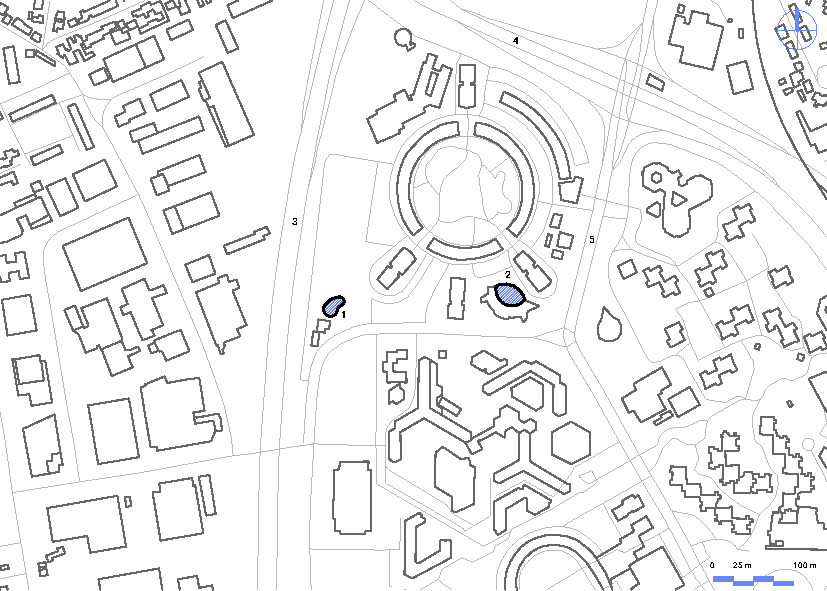
\includegraphics[width=\tmpwidth]{situation_map}}
		\intersectnode{PPtl |- CAtl}{Pt}
		\Photo[
			node=Pt,
			anchor=north west,
			xshift=0mm,
			gopt={width=\tmpwidth},
			]{situation_map}%
		\savenodes{A}
		\Photo[
			node=CAbr,
			anchor=south east,
			xshift=-2\PhotoBigSkip,
			% yshift=\PhotoSkip,
			gopt={height=3.75cm},
			]{form}%
		\savenodes{B}
		\intersectnode{CAtl |- Abr}{Pt}
		%%
		\PhotoCaptionRef[
			hrefnode=Atl,
			node=Atr,
			anchor=south east,
			yshift=\PhotoRefSkip,
			phantom=true,
			]{figure}{Situation map}{Situation map of the cathedrale}{fig:situation_map}
		\PhotoTextBox[
			node=Pt,
			anchor=north west,
			yshift=-\PhotoBigSkip,
			% width=6cm,
			border=false,
			]{%
				\figurecaption[The temporary gridshell (1) was built very close to the permanent cathedral (2). Remark that  the two buildings cover a quite similar projected area.]{fig:situation_map}
			}
		%%
		\PhotoCaptionRef[
			hrefnode=Btl,
			node=Bbr,
			anchor=north east,
			yshift=-\PhotoRefSkip,
			phantom=true,
			]{figure}{Architectural sketch}{Architectural sketch (T. Gray)}{fig:form}
		\PhotoTextBox[
			node=CAbl,
			anchor=south west,
			border=false,
			]{%
				\figurecaption[\raggedright Major and minor volumes are agglomerated into one volume. Here, the morphological register allowed by elastic gridshells appears to be relevant.]{fig:form}
			}
	}
}



\subsection{Context and challenges}
%----------------------------------------------
Creteil is a city of 90.000 inhabitants in the southeast suburb of Paris. Its urbanization began in the late 50’s, impelled by the French architect Charles-Gustave Stoskopf. In 1976 he designed \emph{Notre Dame of Créteil}, a modest catholic church made of concrete, which became a cathedral 10 years later (see item 2 in \cref{fig:situation_map}). Recently, the diocese of Créteil has undertaken a major architectural redevelopment project of its cathedral, including a timber shell covering the religious area and the creation of a new cultural area. Once transformed, the edifice shall be more visible, more hospitable and livelier for citizens. Inevitably, such a molt takes time and a temporary place of worship was required to ensure liturgical services during the two-years work. In November 2011, T/E/S/S, the structural design office in charge of the cathedral renovation project, made an ambitious proposal to the diocese~: based on a previous successful experience – the construction of a composite gridshell for the festival Solidays \cite{Baverel2012} – T/E/S/S suggested that rather installing a basic tent, the parishioners should construct themselves a temporary cathedral.\footnote{See the video of the construction of Solidays' gridshell here : \url{https://youtu.be/24LLfcVIZWw}.}\textsuperscript{,}\footnote{See the video of the construction of Creteil's gridshell here : \url{https://youtu.be/jLq-UfOdnQQ}.}

% \begin{figure}[t]
% 	\centering
% %	\begin{fullpage}
% 		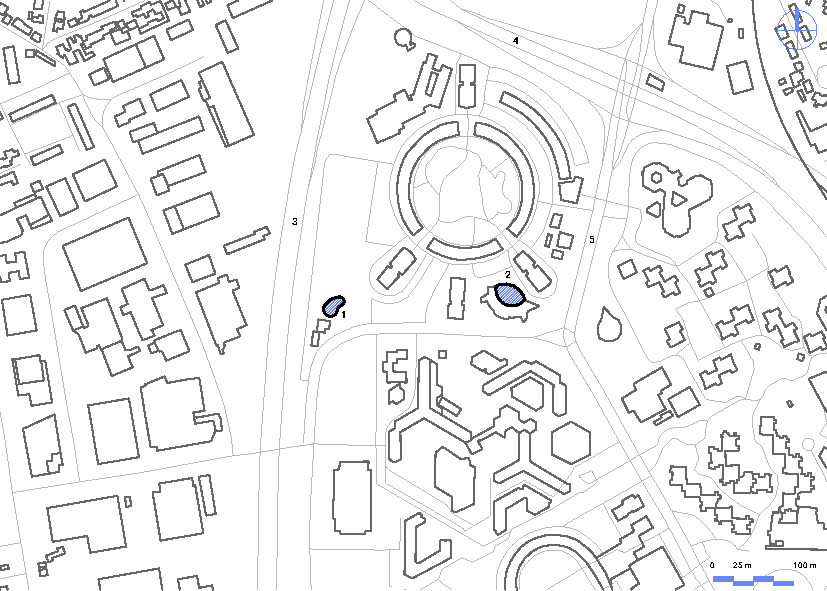
\includegraphics[width=1\textwidth]{situation_map}
% 		\caption[Situation map]{Situation map. The temporary gridshell (1) was built very close to the permanent cathedral (2). Remark that  the two buildings cover a quite similar projected area.}
% 		\label{fig:situation_map}
% %	\end{fullpage}
% \end{figure}

\subsection{Architectural considerations on the form}
%------------------------------------------------------------------
The origin of this building form was driven by two objectives, that is, to provide a variety of appropriate internal spaces within which the community could assemble, and to provide an externally welcoming and visually interesting form. According to the architect Tom Gray, today, the internal organization of a roman catholic church is in large part driven by the post Vatican II vision of a religious celebration being a collective gathering of the community around the Eucharist, center of spiritual life. A circular seating arrangement is often considered the most convivial form to create a sense of belonging while minimizing a sense of hierarchy. However the community is not only using the building for religious celebration but also for encounters on a more informal manner, for example spontaneous gatherings after religious ceremonies. In the early Roman church, such gathering of the community was facilitated by the presence of an anti-space to the main space called a \emph{narthex}, through which one passed on entering the church. It was therefore felt appropriate that the formal freedom which the gridshell system offered would be used to explore forms composed of an agglomeration of major and a minor volumes which contain the two functions~: formal and informal gatherings (see item 1 and 2 in \cref{fig:form}).

Formal explorations were undertaken using modeling clay. The final form is based loosely on two adjacent semi spherical volumes of different size, which are merged into one complex form. Externally the fear of the design team was that the totally convex blob form could look intimidating. It was therefore decided that the two spherical virtual forms, which would be joined to make the final form, would be arranged not in a symmetrical axial manner, but in an asymmetrical curved composition. The resulting form seen in plan is convex on one side and concave on the other. The concave form in plan allows for double curvature to be introduced into what would be otherwise a simpler blob and gives sensuality and visual interest to the building.

% \begin{figure}[t]
% 	\centering
% 	\begin{fullpage}
% 		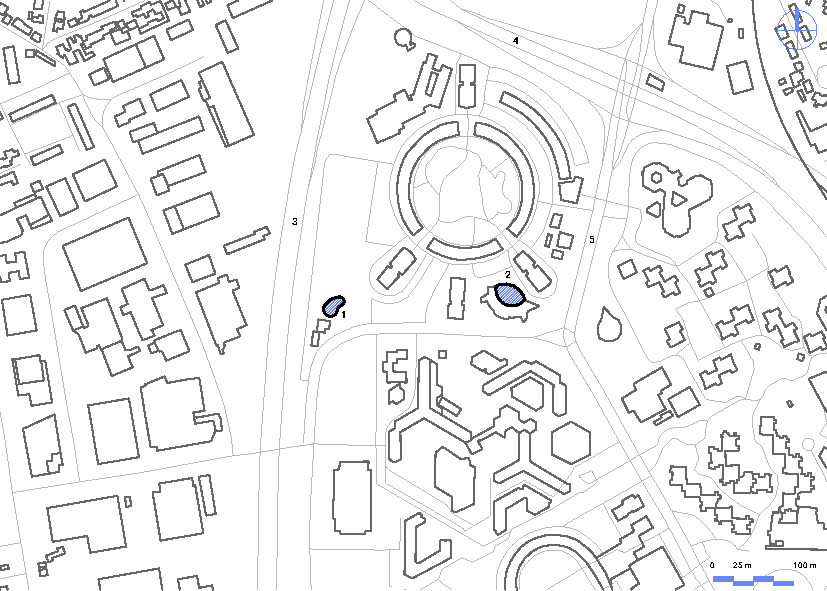
\includegraphics[width=1\textwidth]{situation_map}
% 		\caption[Situation map]{Situation map. The temporary gridshell (1) was built very close to the permanent cathedral (2). Remark that  the two buildings cover a quite similar projected area.}\label{fig:situation_map}
% 		\vspace{1.5cm}
% 		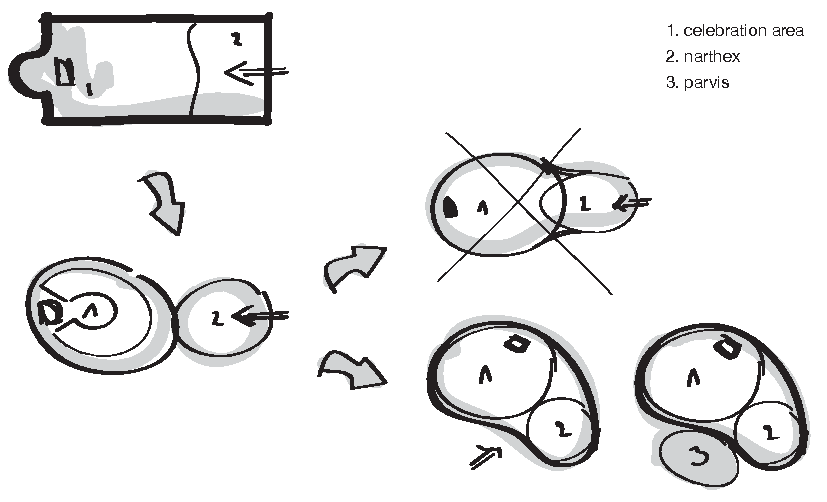
\includegraphics[width=0.7\textwidth]{form}
% 		\caption[Architectural sketch]{Architectural sketch (T. Gray). Major and minor volumes are agglomerated into one volume. Here, the morphological register allowed by elastic gridshells appears to be relevant.}\label{fig:form}
% 	\end{fullpage}
% \end{figure}

% \begin{figure}[p]
% 	%
%      	\centering
% 	\begin{leftfullpage}
% 		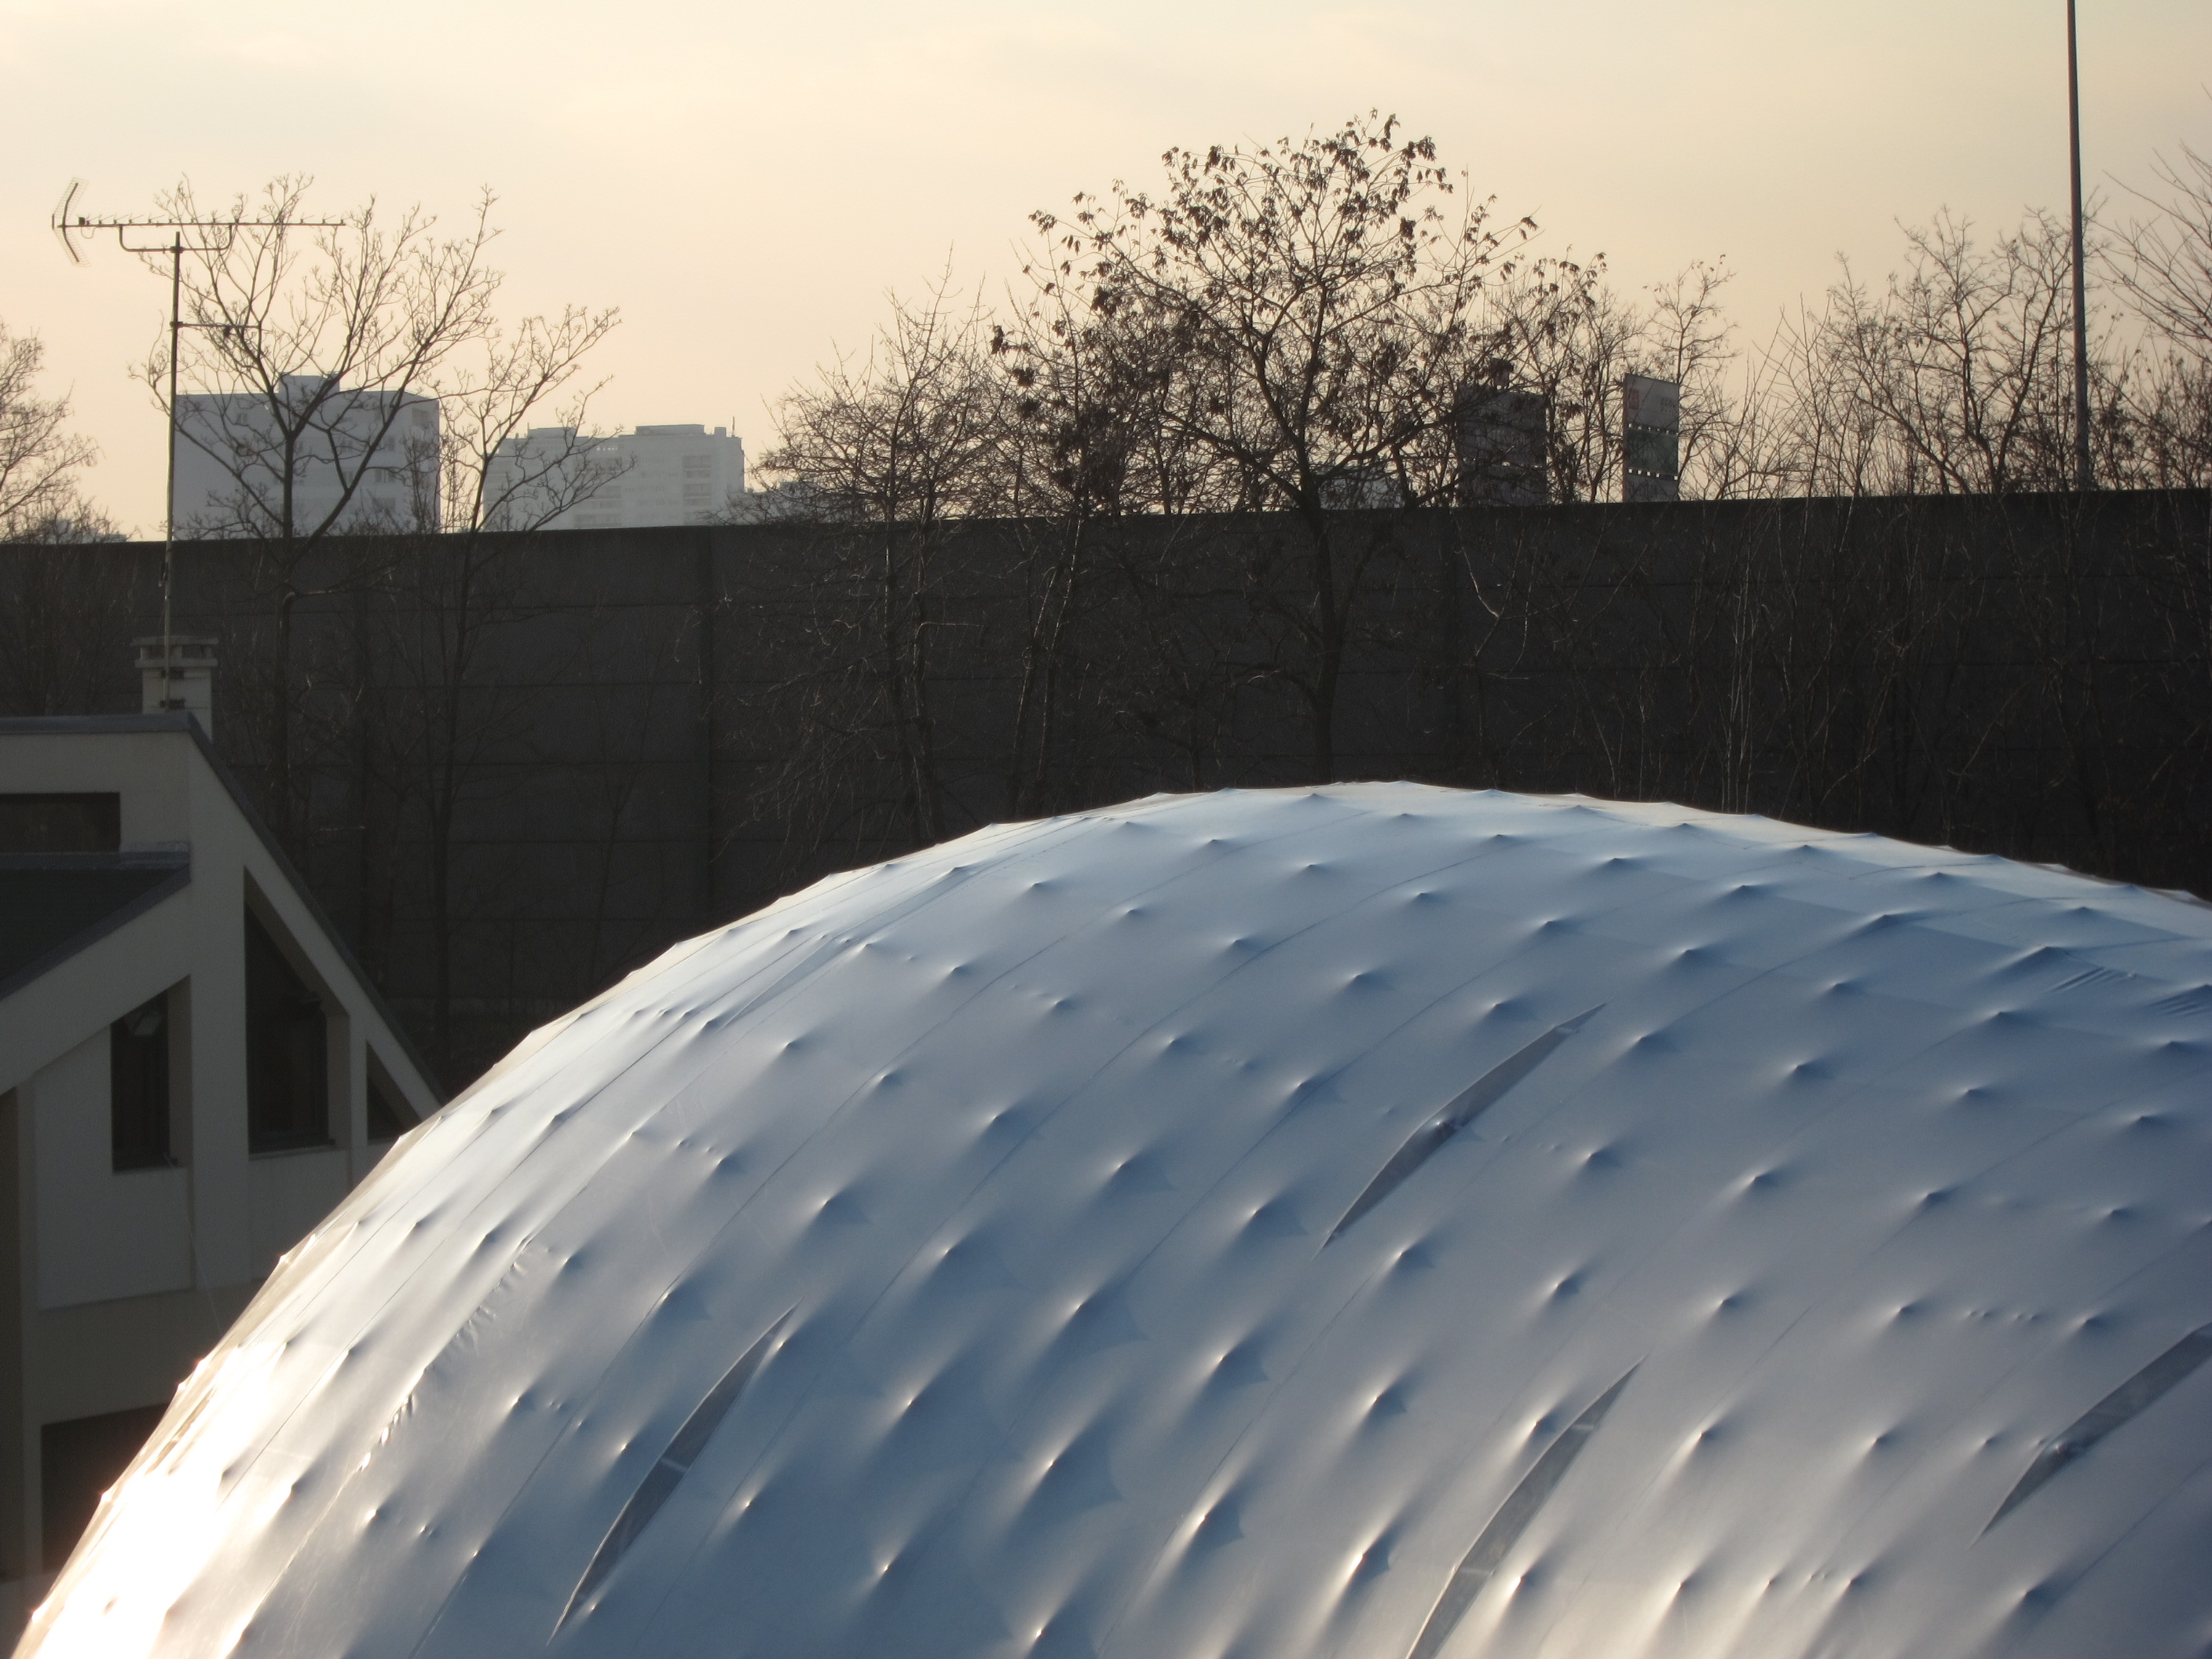
\includegraphics[width=0.80\textwidth]{gs_ext.jpg}
% 		\caption[Exterior view]{Exterior view. The connections mark the fabric suggesting the interior grid structure. This texture enriches the perception of the building viewed from the outside and creates effects with the light reflections -- \textcopyright~L. du Peloux for T/E/S/S.}
% 		\label{fig:gs_ext}
% 		\vspace{1cm}
% 		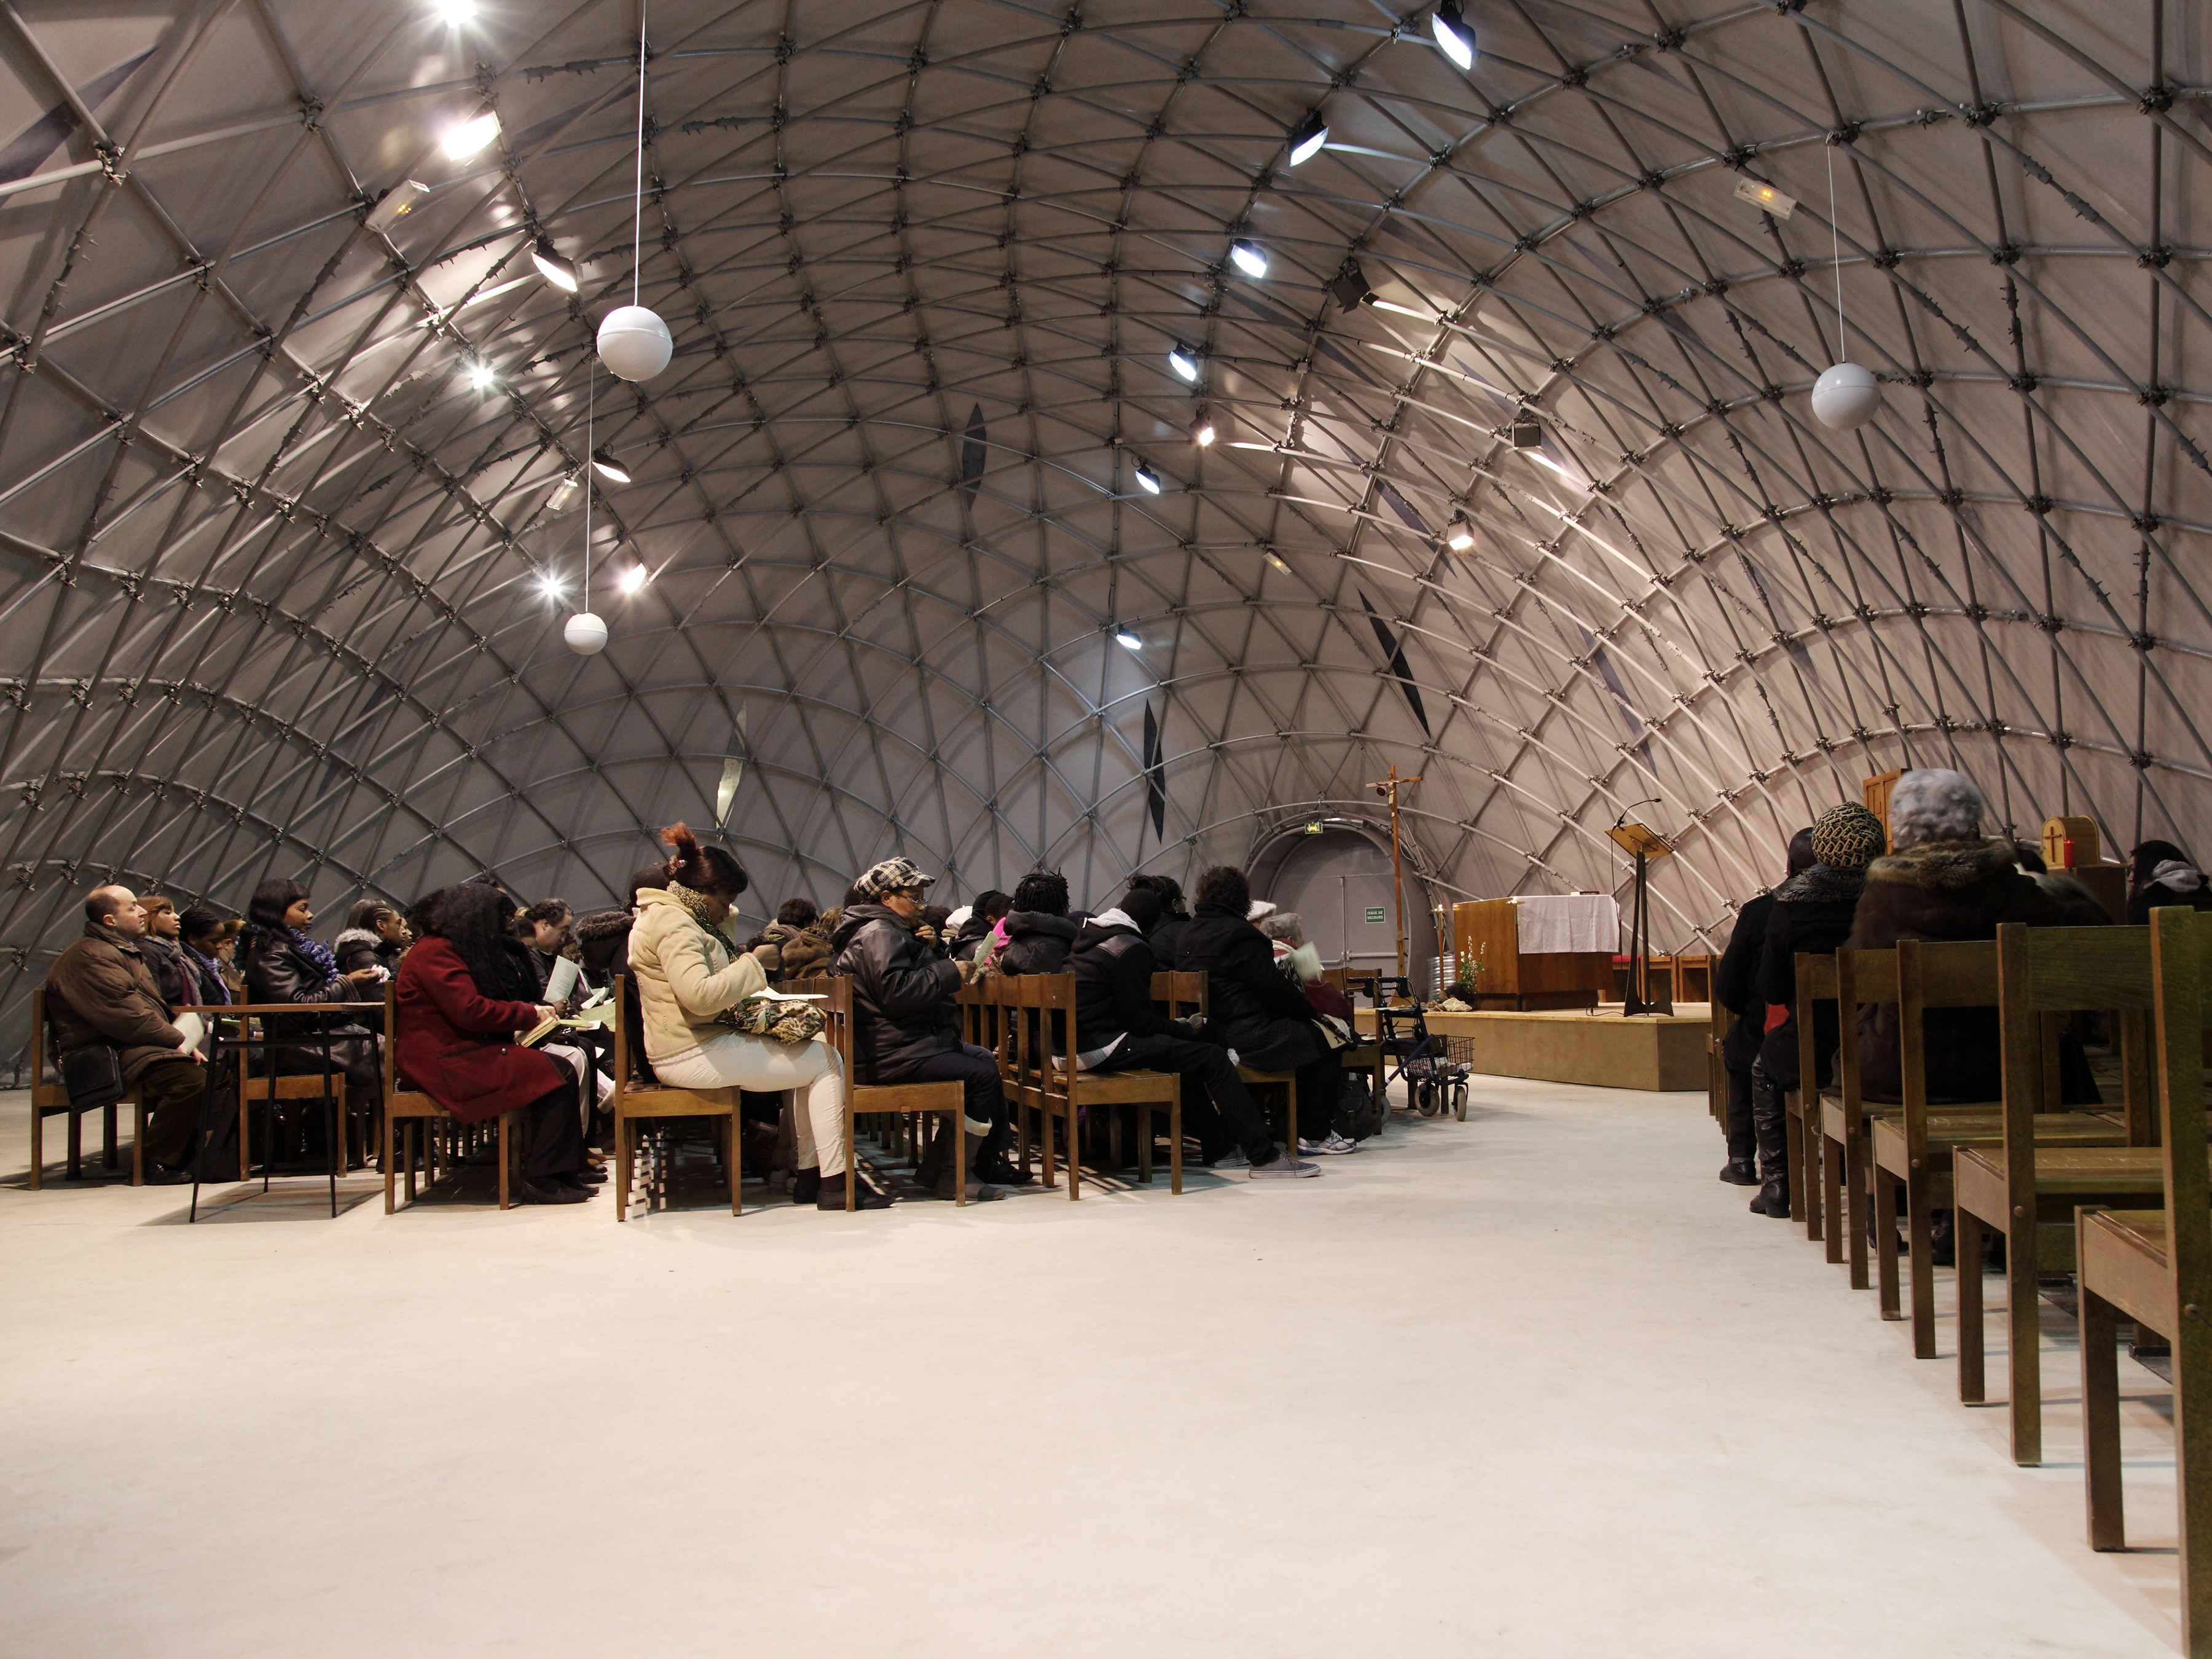
\includegraphics[width=0.80\textwidth]{gs_int.jpg}\label{fig:gs_int}
% 		\caption[Interior view]{Interior view. The grid pattern highlights the lightness of the structure and gives its tempo to the internal space. Lines converge to the altar, the heart of the liturgical area where the mass is offered on -- \textcopyright~C. Moissinac for T/E/S/S.}
% 		\vspace{20pt}
% 	\end{leftfullpage}
% \end{figure}

% \begin{figure}[p]
%      	\centering
% 	\begin{fullpage}
% 		%
% 		\subfloat[][Exterior]{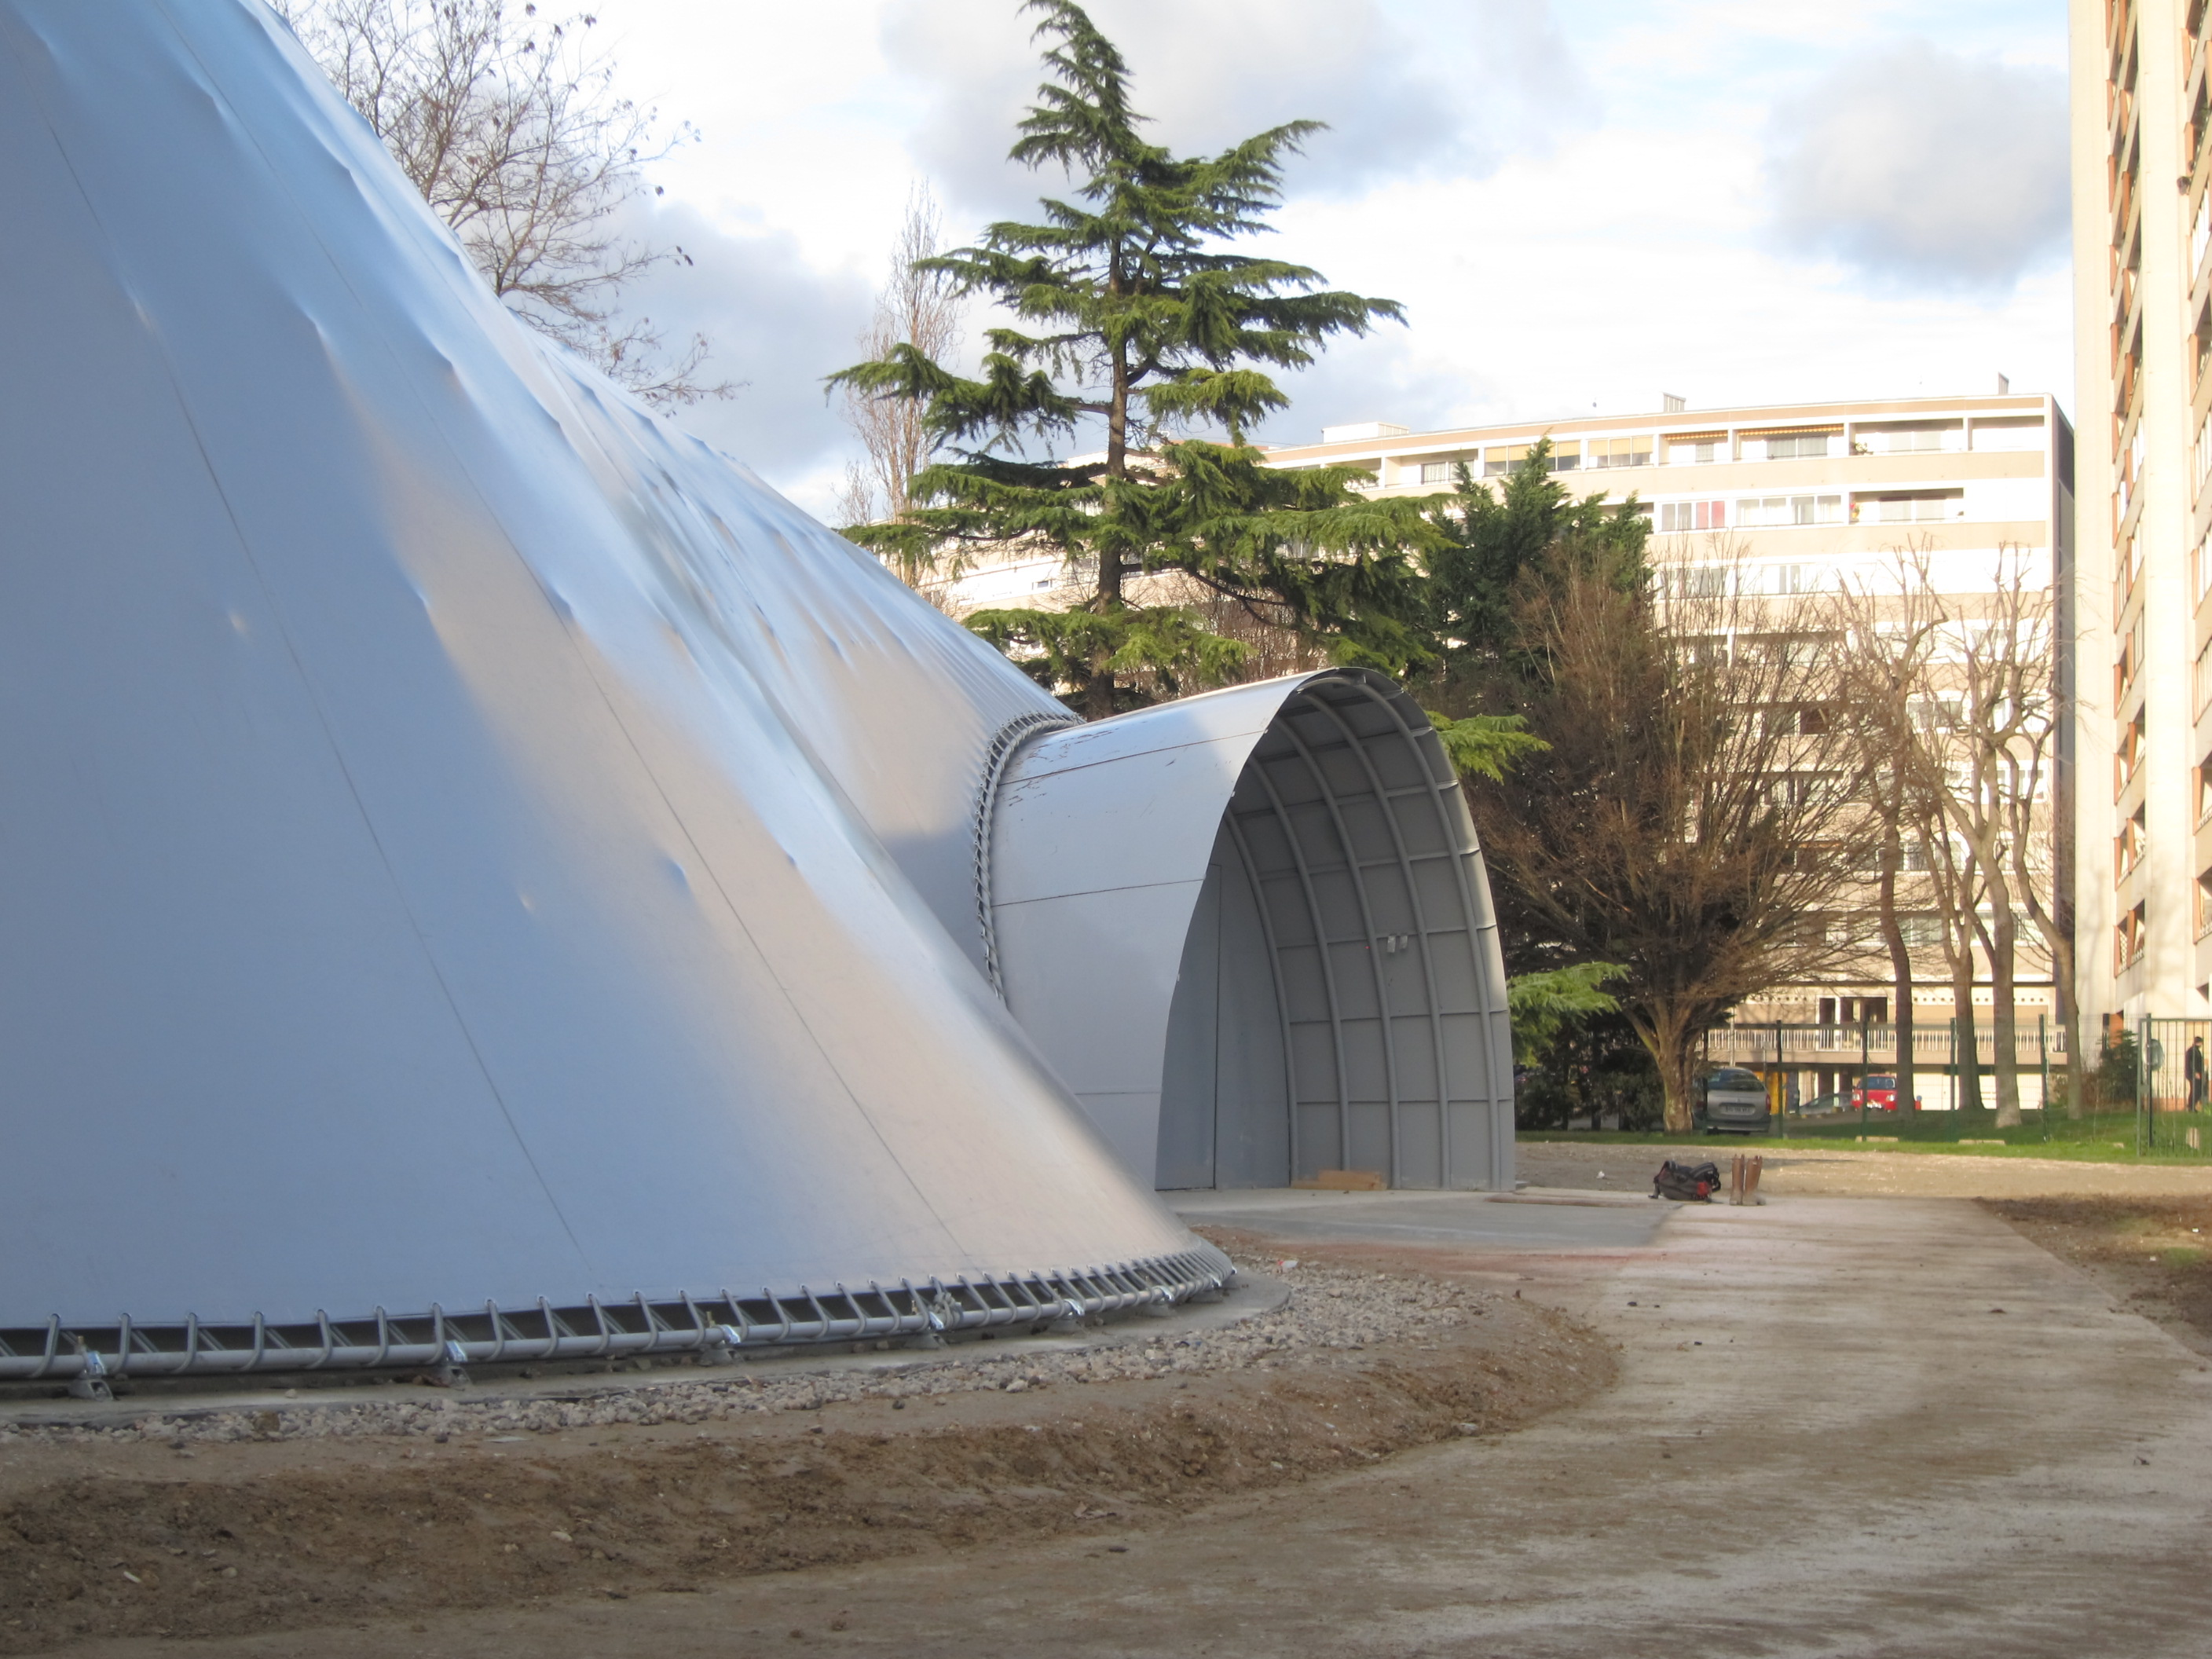
\includegraphics[width=0.48\textwidth]{door_ext.jpg}\label{fig:door_ext}}
% 		\hspace*{\fill}
% 		\subfloat[][Interior]{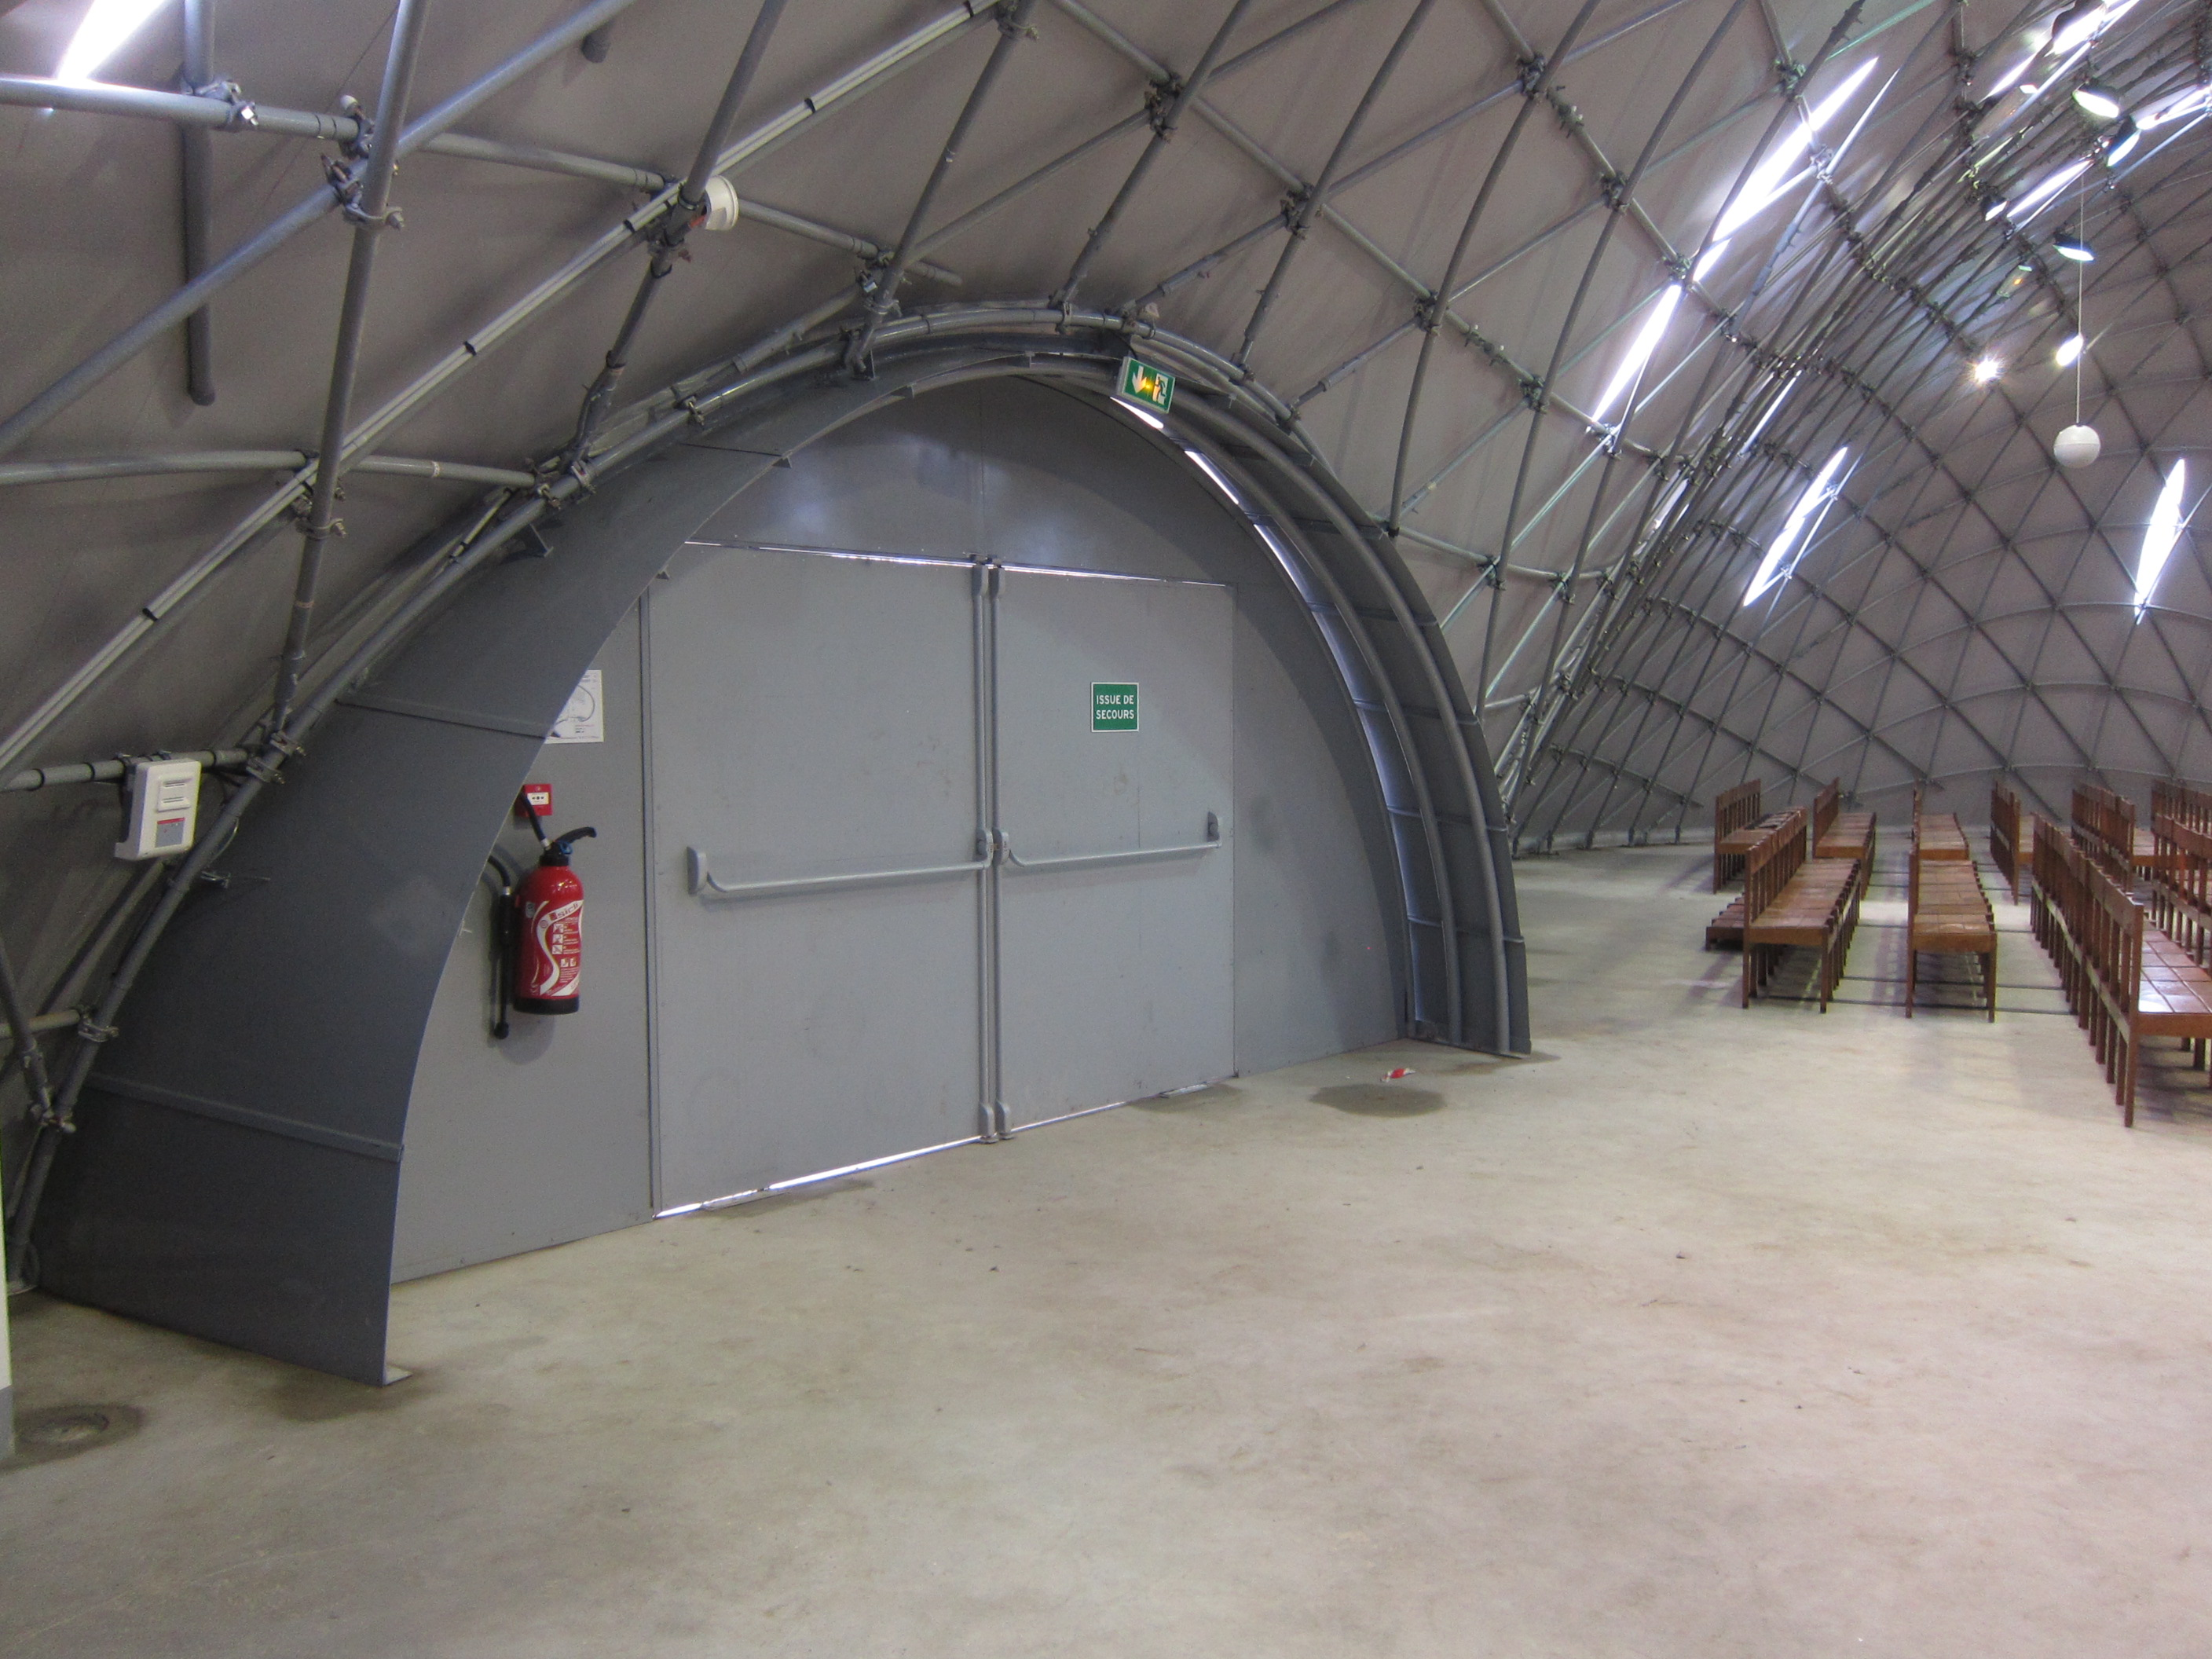
\includegraphics[width=0.48\textwidth]{door_int.jpg}\label{fig:door_int}}
% 		\vspace{10pt}
% 		\caption[Entrance]{Entrance. Two steel doors allow the entrance inside the building.}
% 		\label{fig:door}
% 		%
%      		\vspace{1cm}
% 		%
% 		\subfloat[][Swivel coupler]{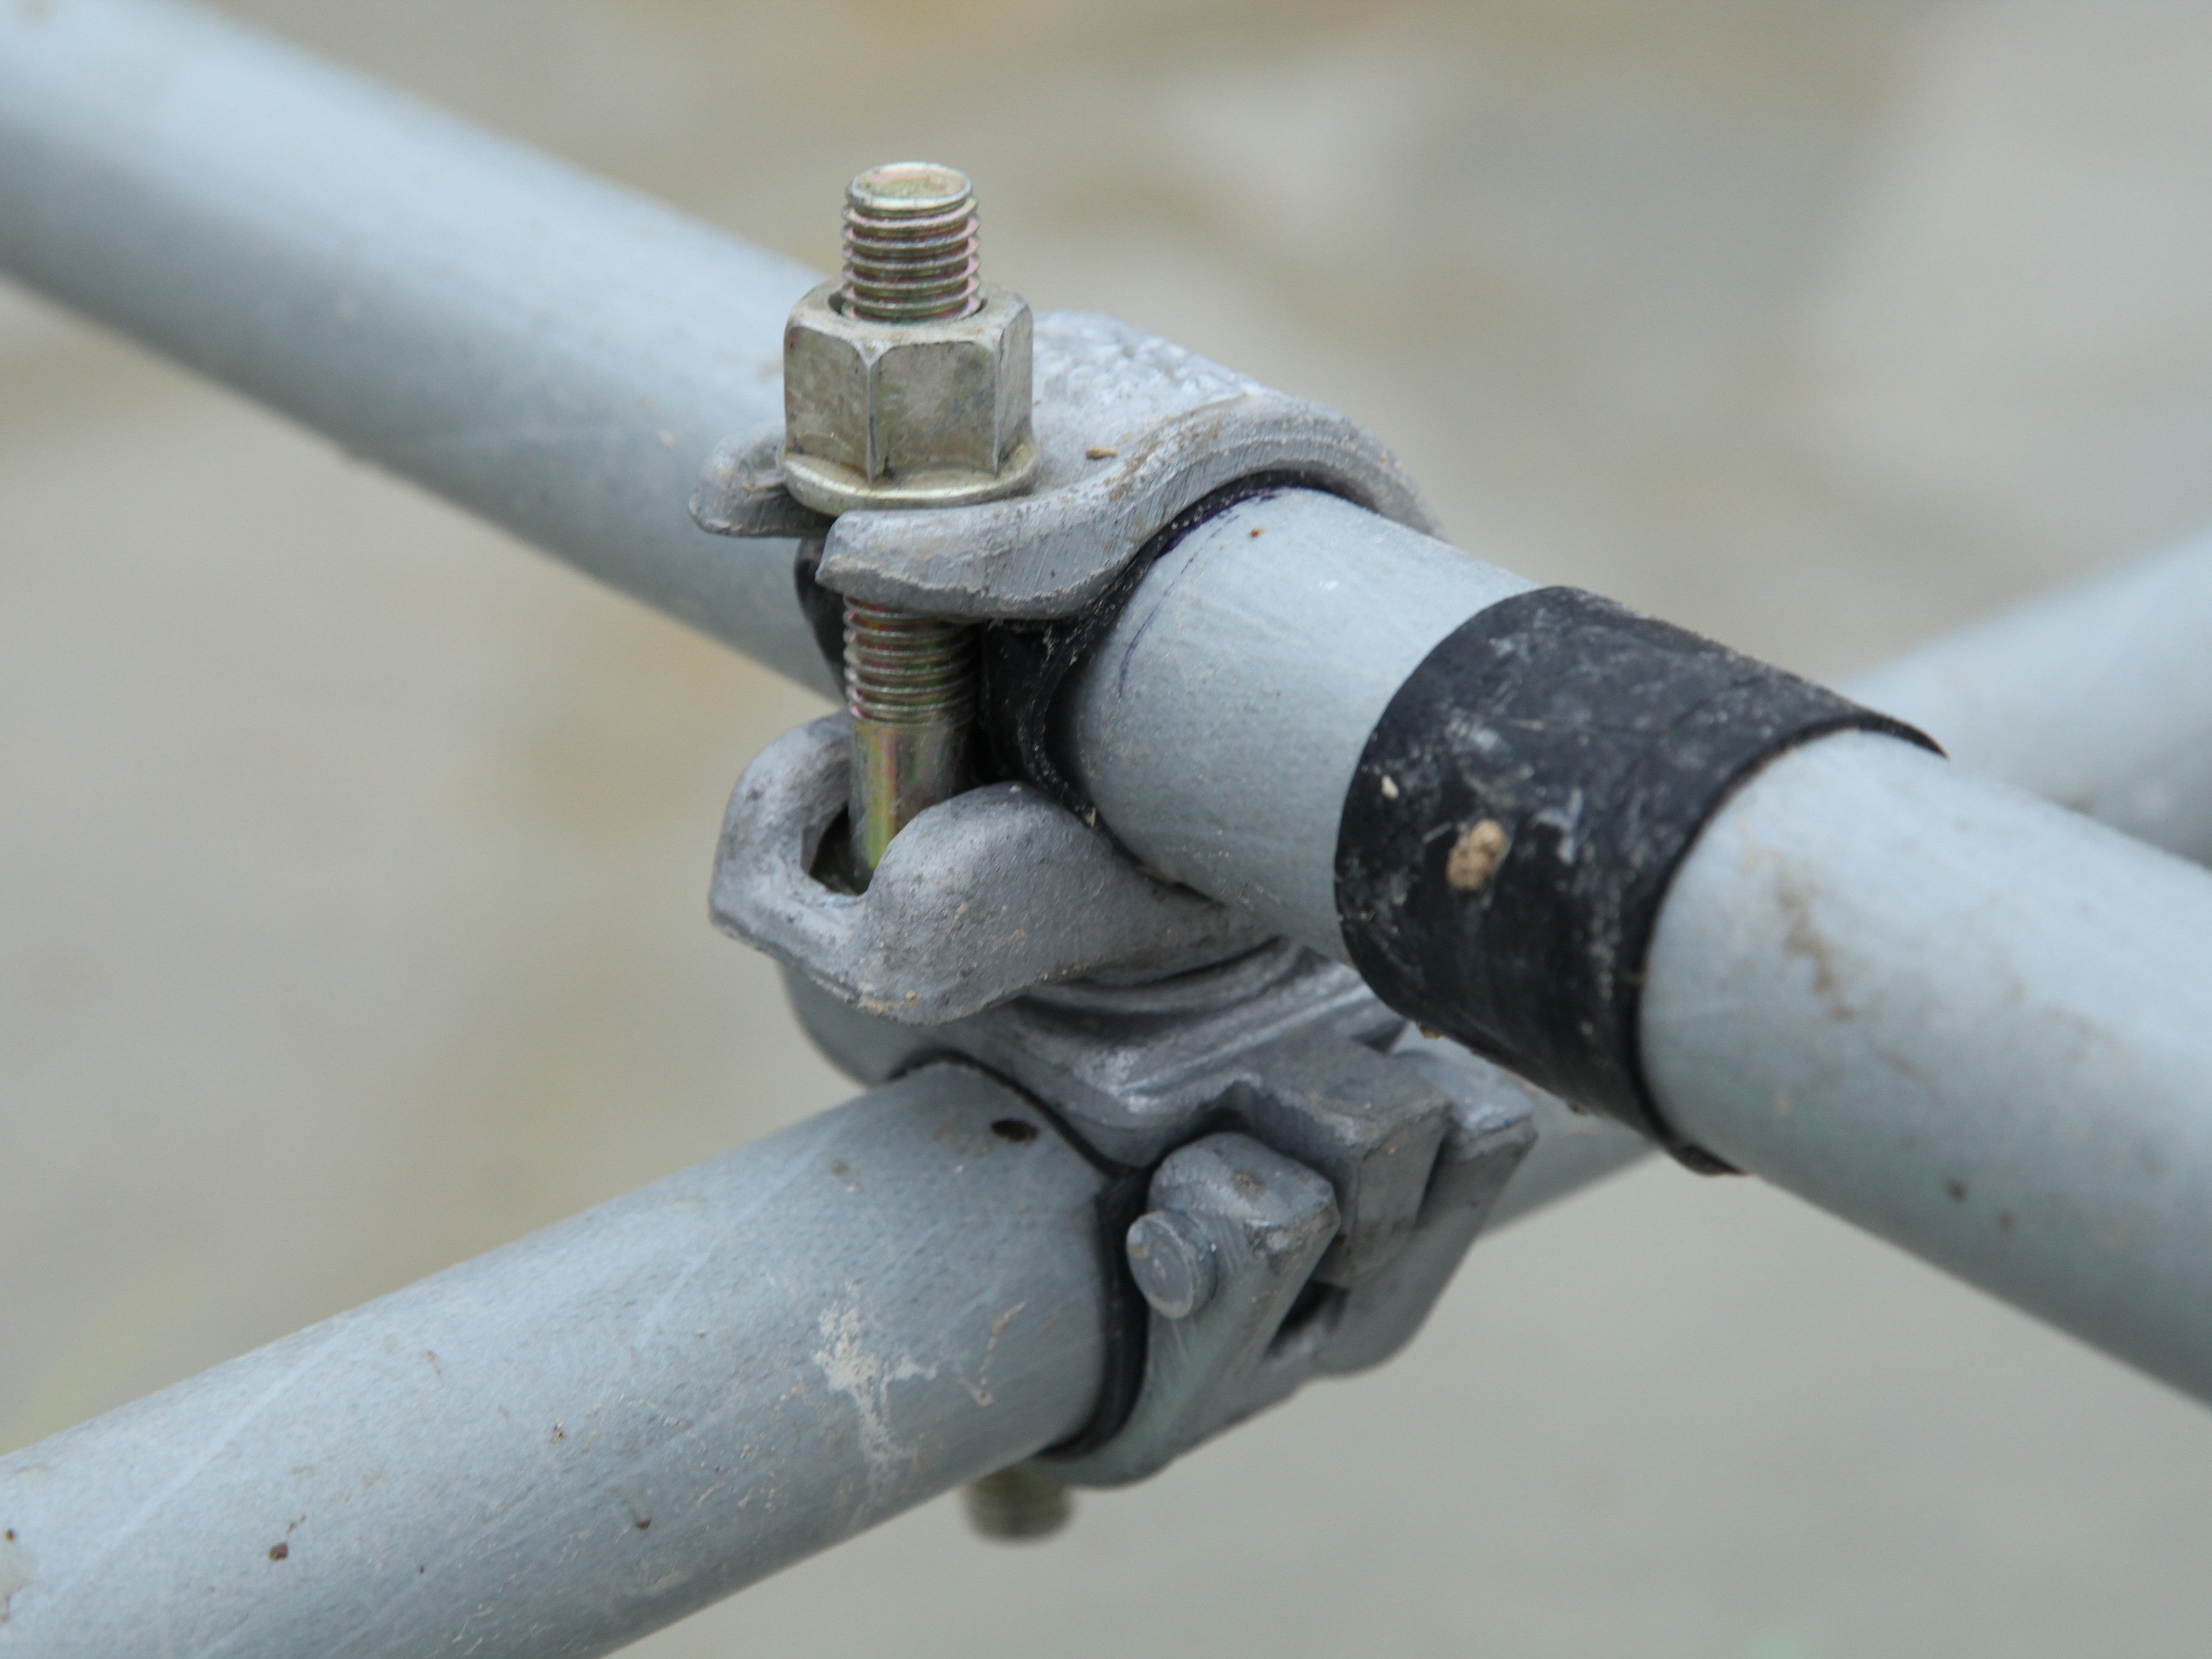
\includegraphics[width=0.48\textwidth]{swivel.jpg}\label{fig:swivel}}
% 		\hspace*{\fill}
% 		\subfloat[][Sleeve system]{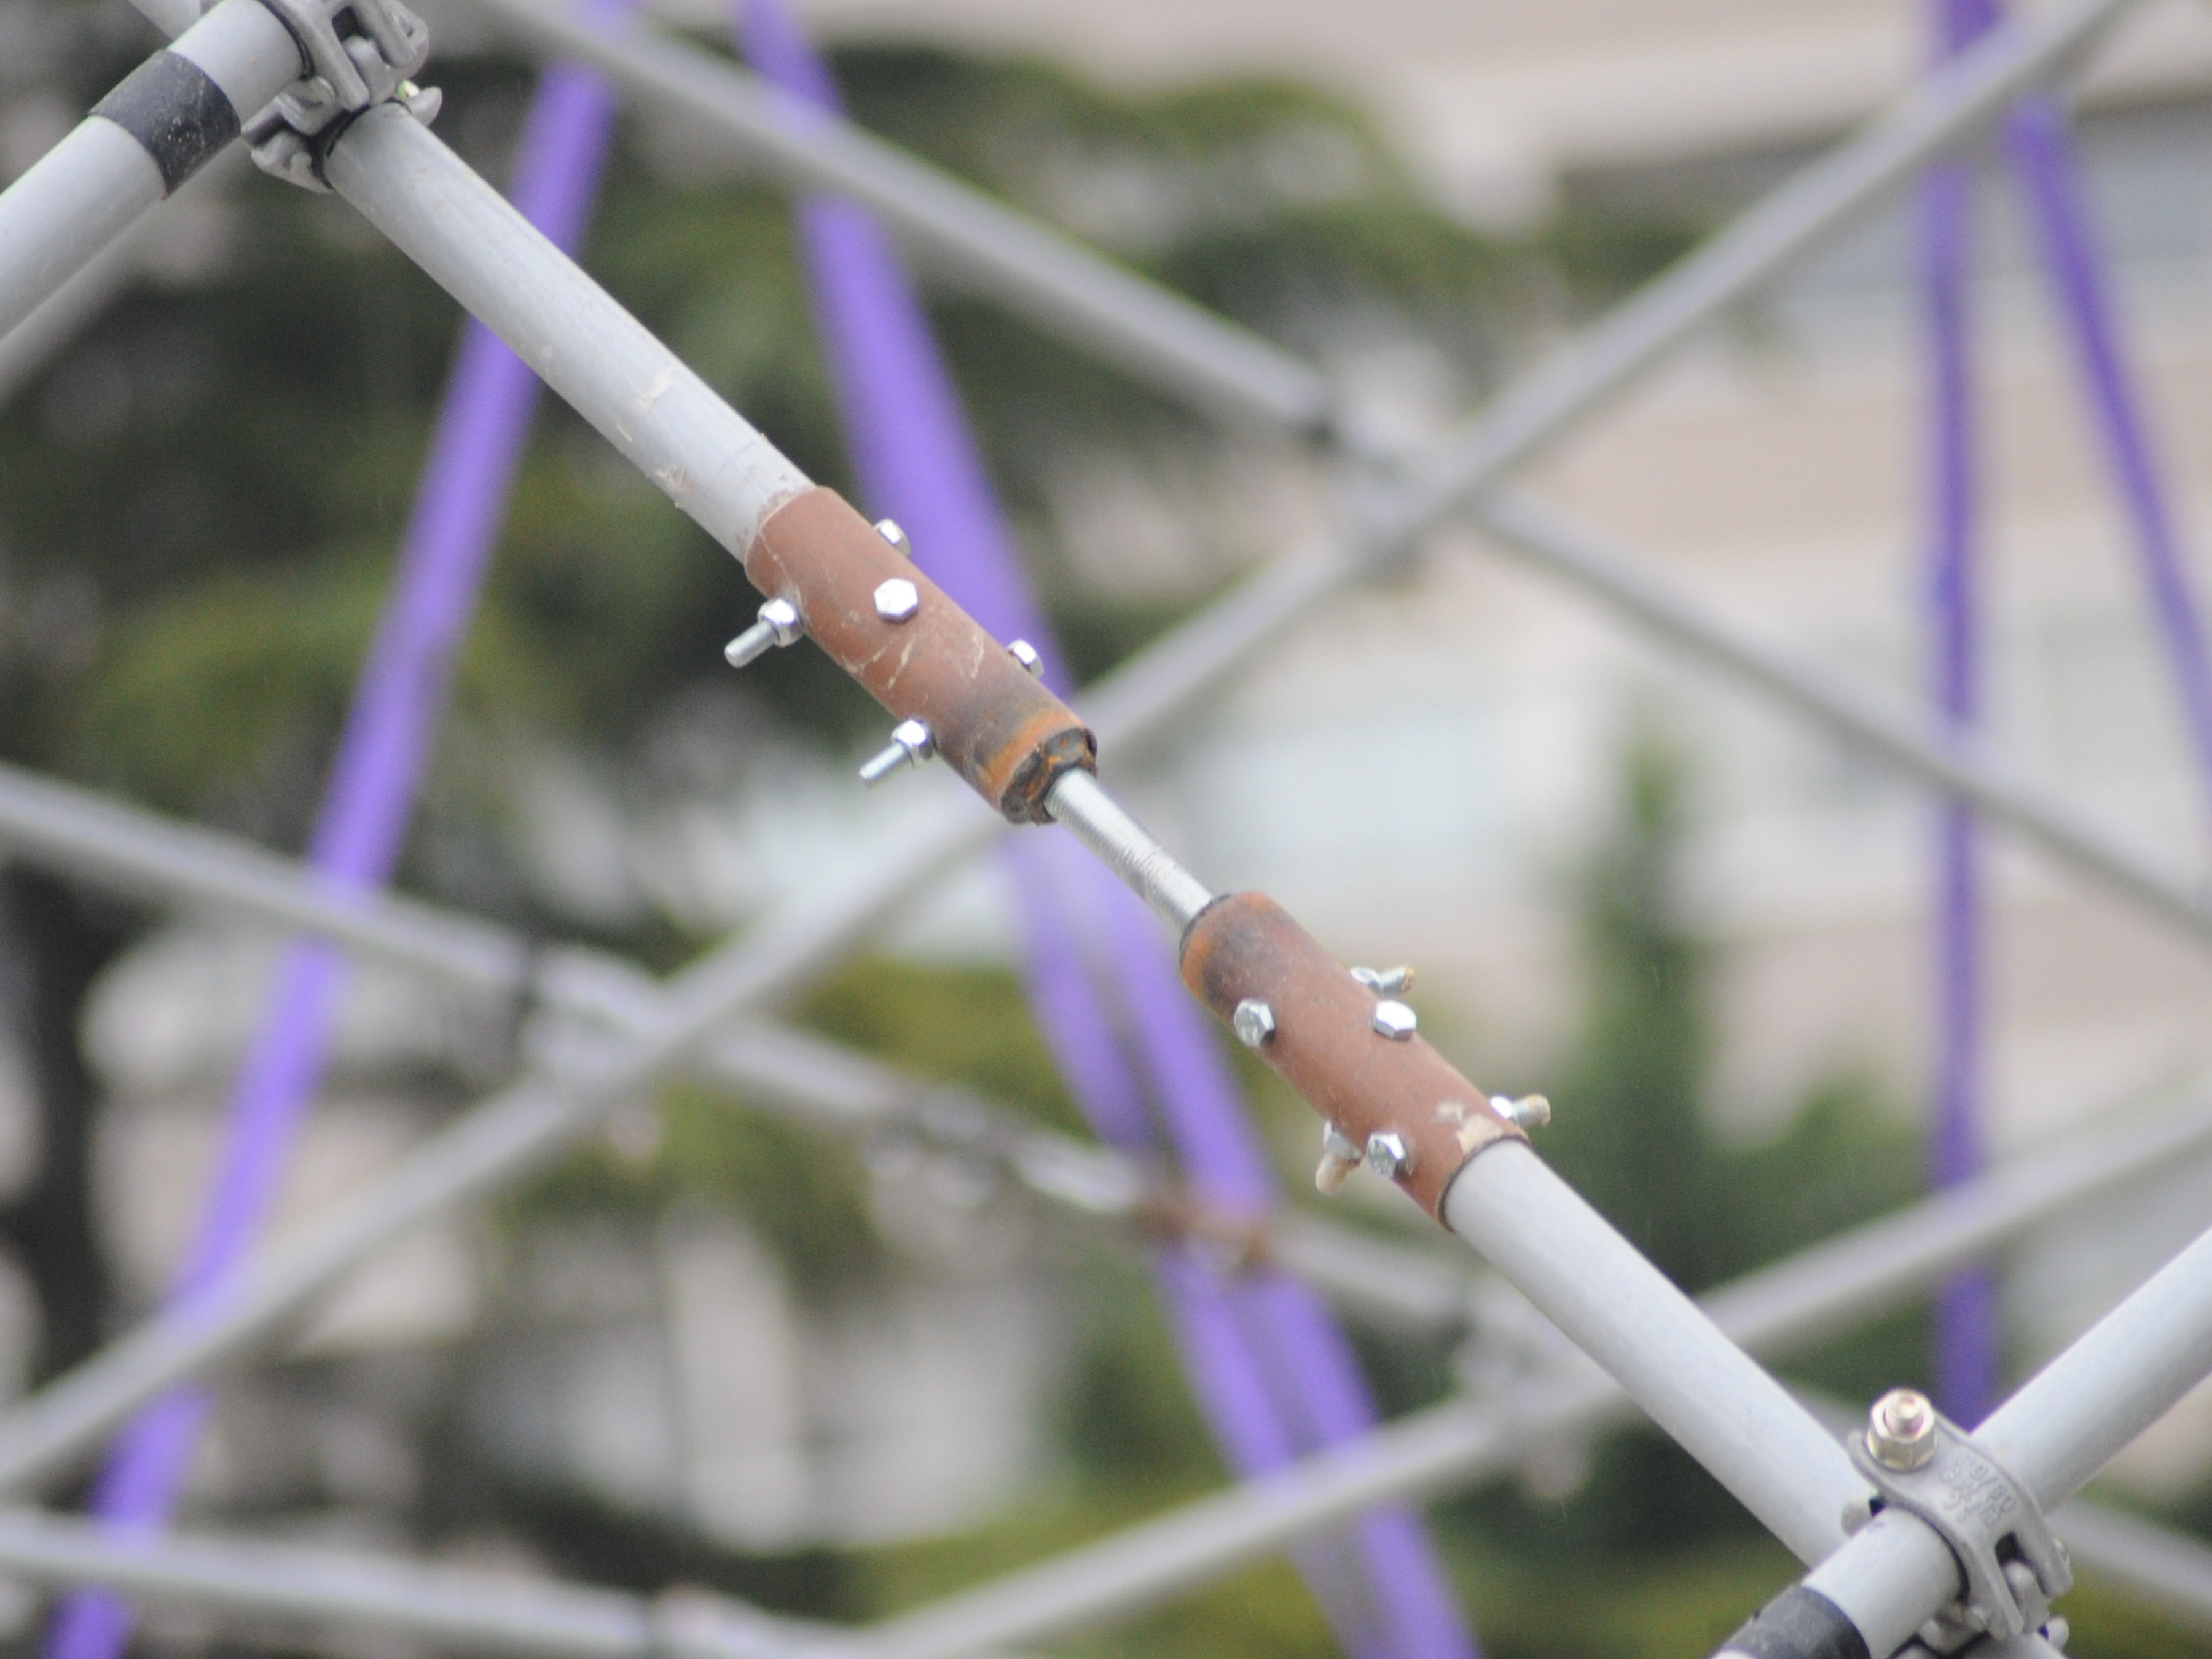
\includegraphics[width=0.48\textwidth]{sleeve.jpg}\label{fig:sleeve}} \\
% 		%
% 		\subfloat[][Ground anchorage]{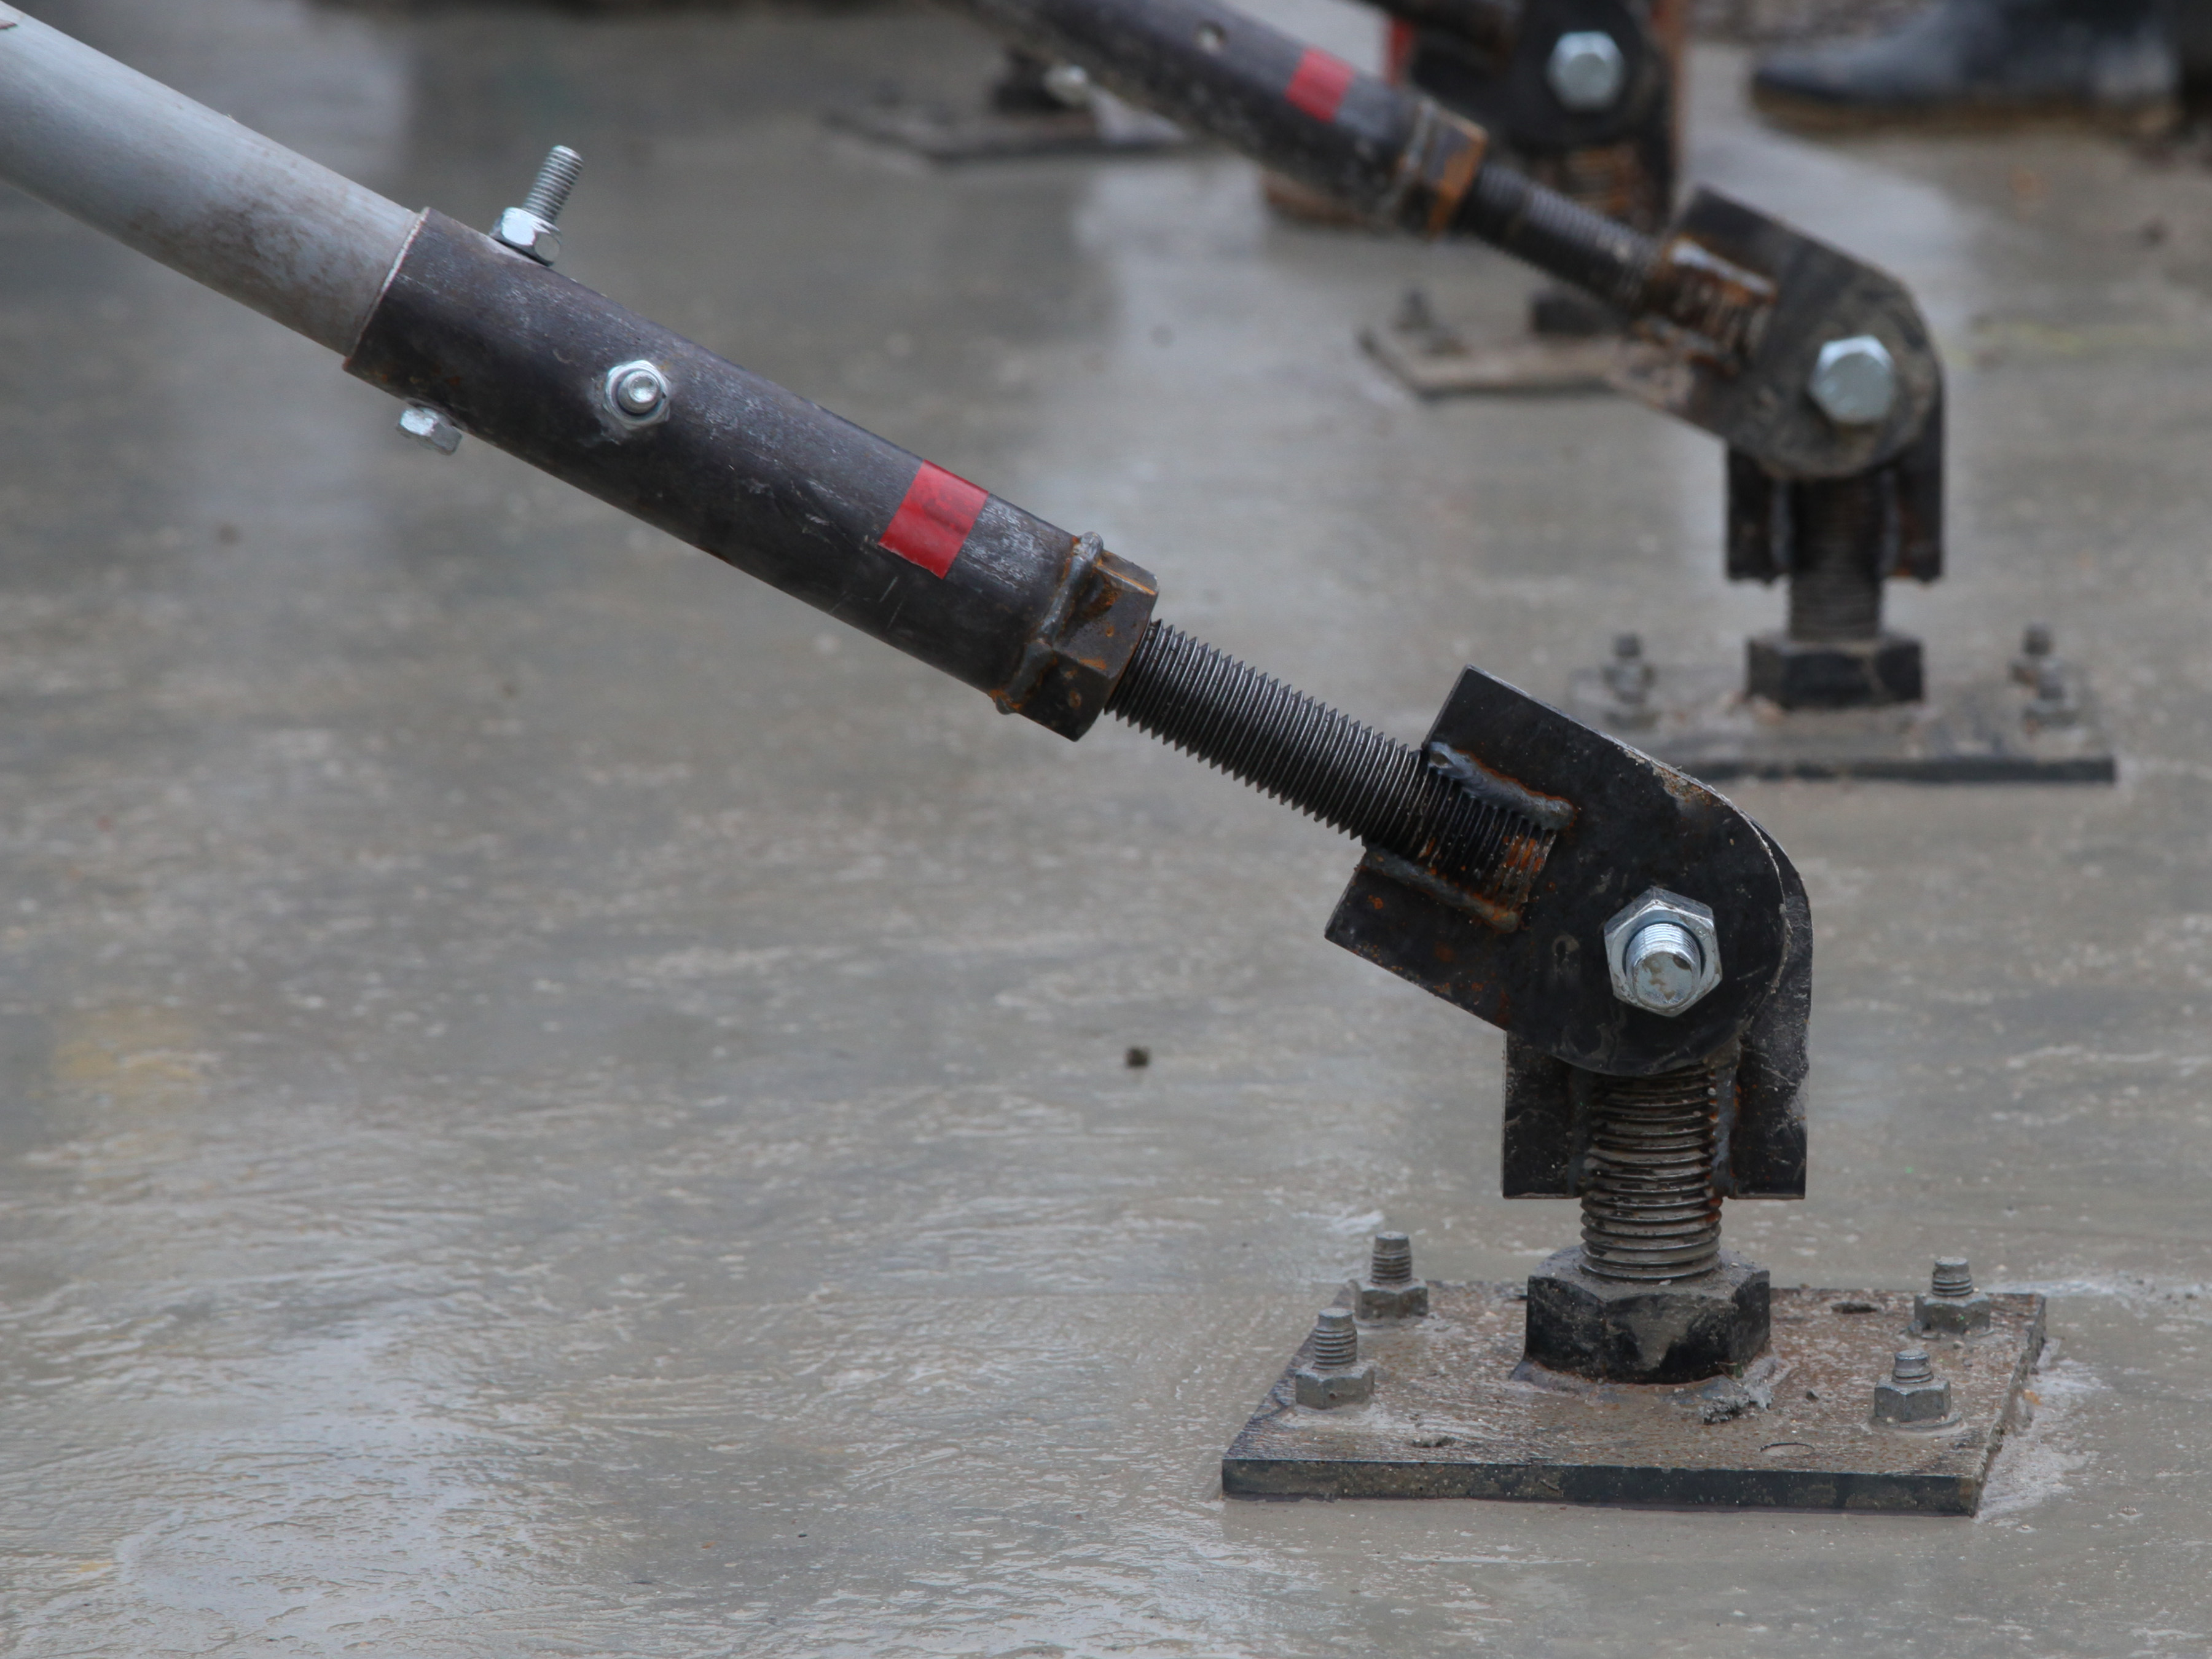
\includegraphics[width=0.48\textwidth]{anchorage.jpg}\label{fig:anchorage}}
% 		\hspace*{\fill}
% 		\subfloat[][Lacing rod]{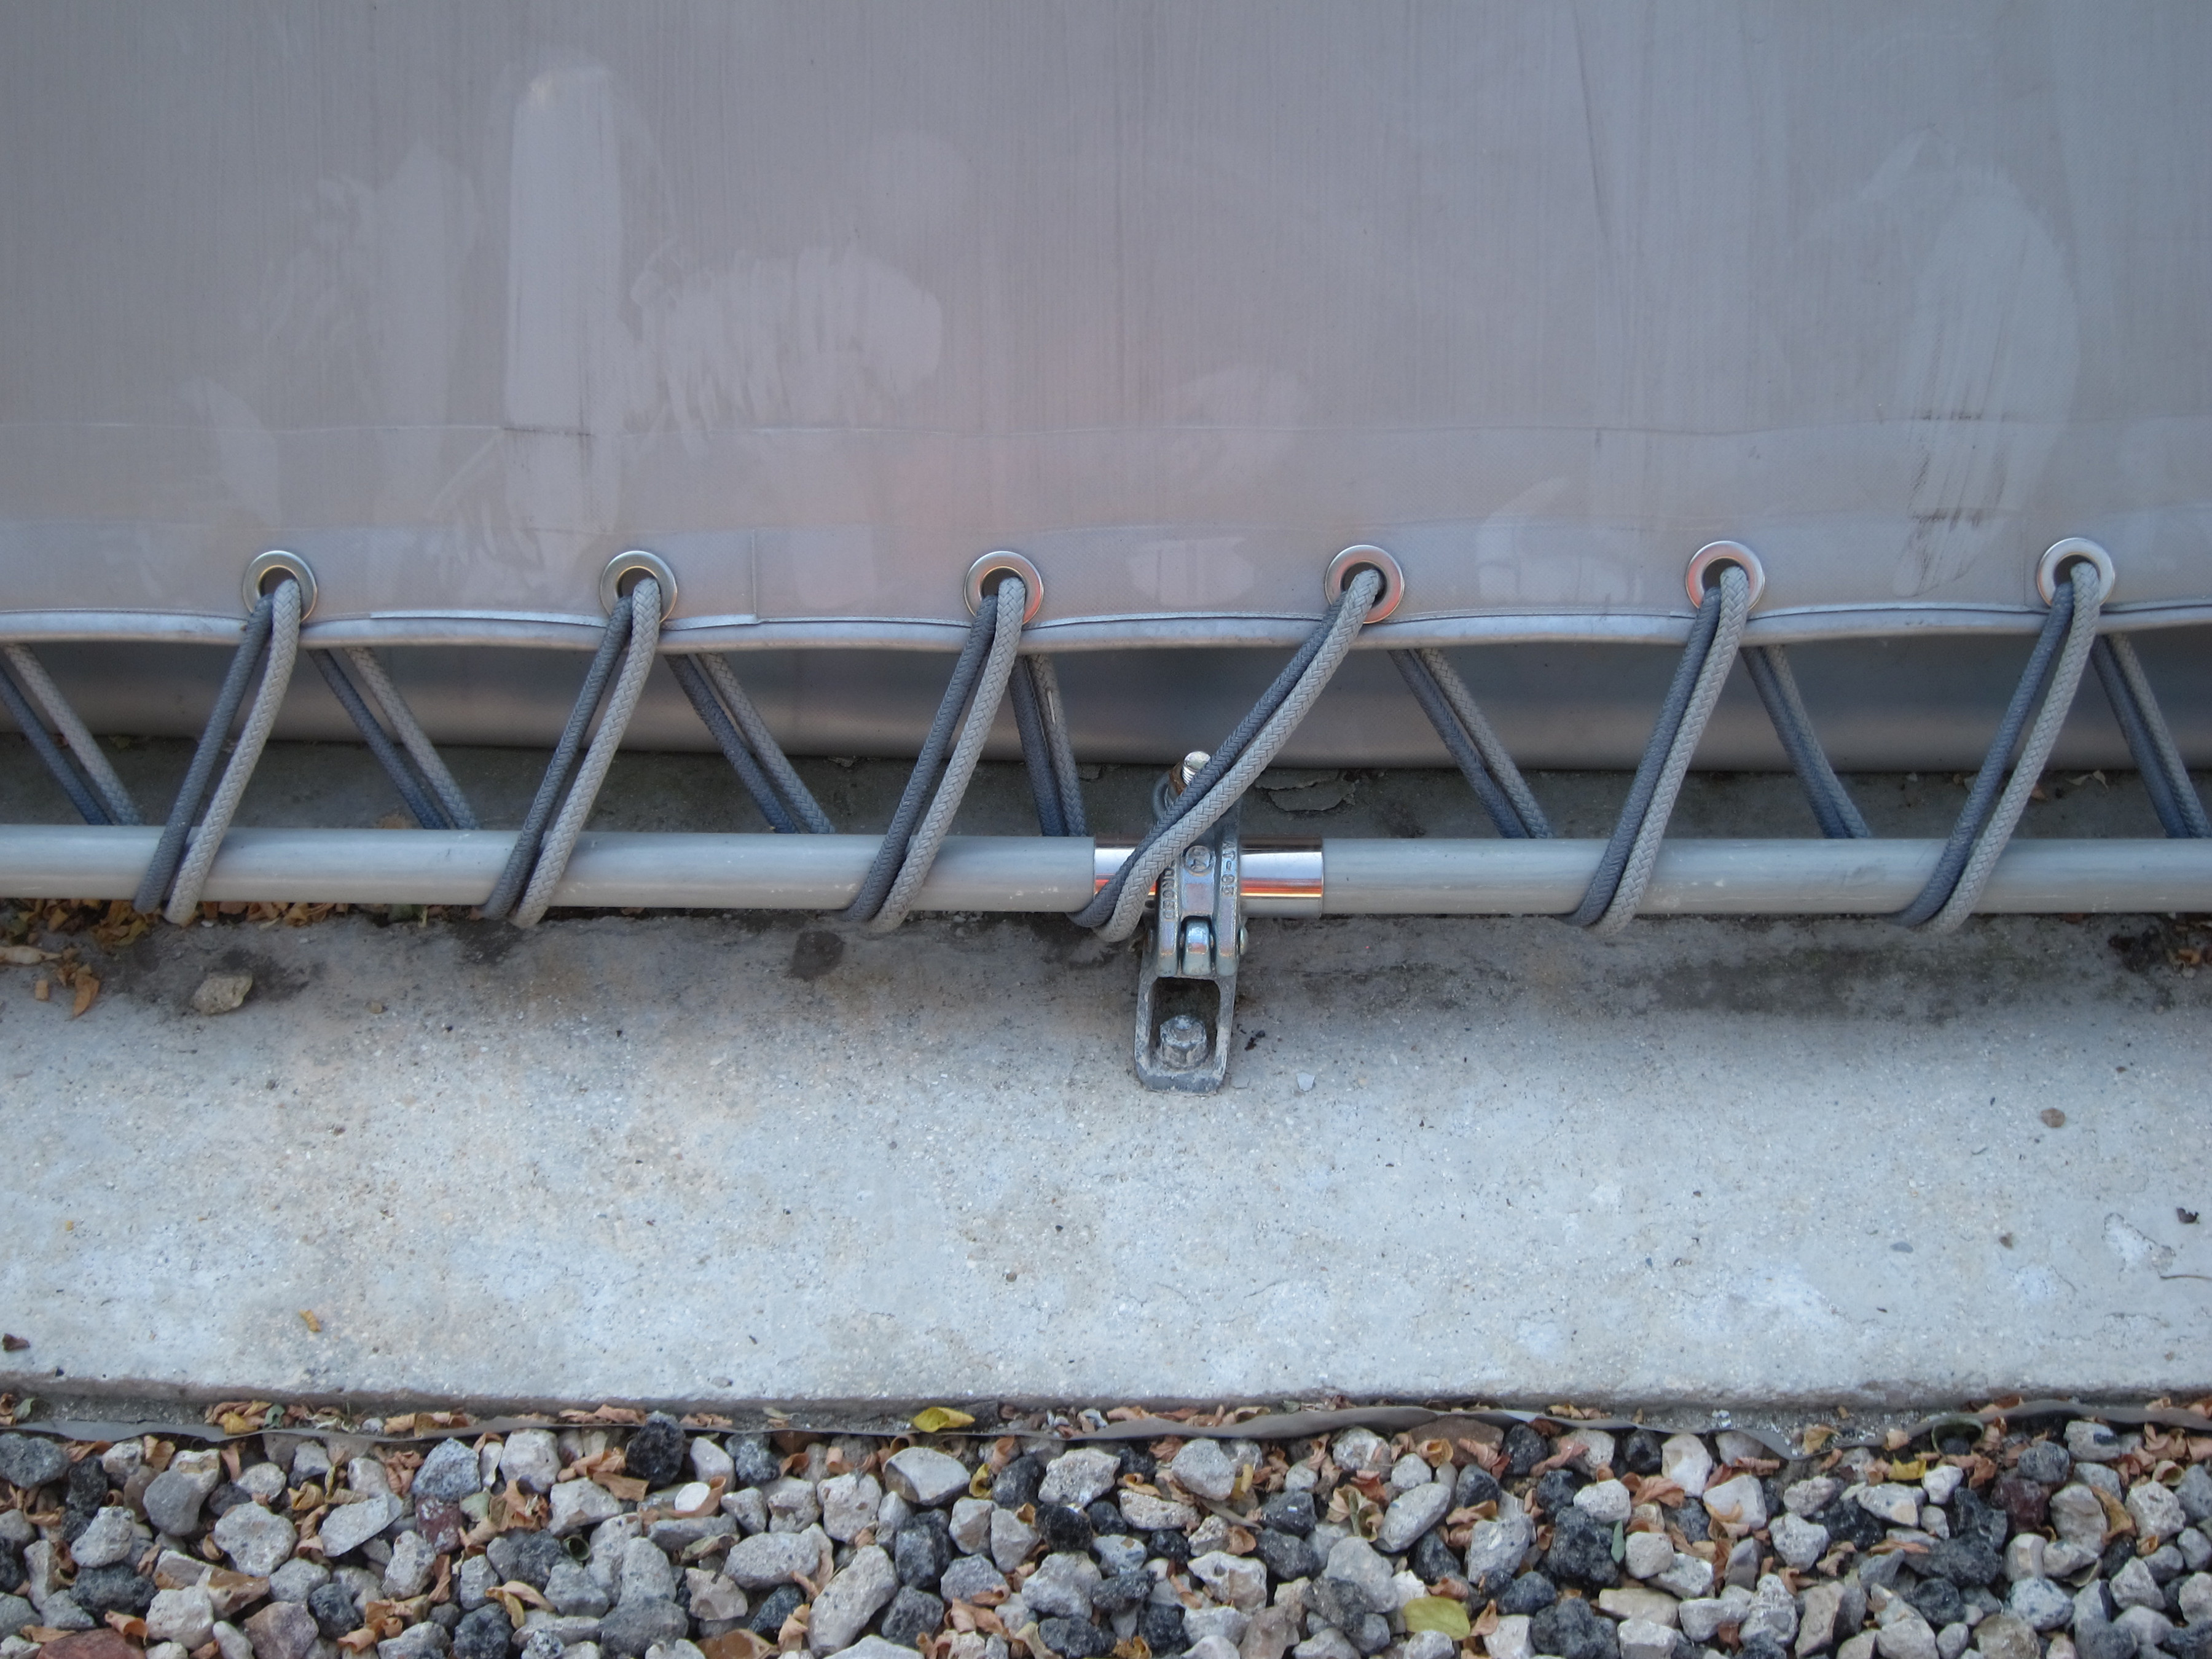
\includegraphics[width=0.48\textwidth]{edge.jpg}\label{fig:edge}} \\
% 		%
% 		\vspace{10pt}
% 		\caption[Key elements of the structural system]{Key elements of the structural system.}
% 		\label{fig:parts}
% 	\end{fullpage}
% \end{figure}

\subsection{Placing of the building on the site}
The temporary cathedral is located on a land owned by the municipality, which is used for sporting and other communal gatherings. The curve in the building defines an external area where the church community could meet in the open air and this is where the entrance to the church is situated. The building was positioned on the site so that the entrance addresses a grass planted area forming a garden forecourt or “parvis” (see item 3 in \cref{fig:form}). A service building housing plant, toilets and vestry are housed in a port cabin positioned to the rear of the building (see \cref{fig:plan_view}).

\subsection{Entrance}
It is formally quite difficult to integrate doors, which must be verticals, into a complex geometry. Either the gridshell could be deformed to accommodate the geometrical requirements of doors, or the doors could be integrated into an independent form. The latter approach was chosen. In looking for forms to house the doors, reference was made to the conical monumental doorways with rings of concentric decoration, which welcome the faithful to romanesque and gothic churches in France. The conical forms were found to be coherent to the overall geometry of the building. The entrance doors were therefore inserted into a conical hooded form made of rolled steel plates and stiffened by concentric steel tubes, which not only make reference to historic precedence but also refer to the gridshell to be discovered inside (see \cref{fig:door_int}). The cone of the entrance doors was positioned in the concave side of the building giving access directly to the narthex part of the internal volume. To the rear of the church is situated a service door. The steel hood, which houses this door, is curved tightly around the door and takes up an ovoid form.

\blankpage{%
	\thispagestyle{empty}
	\hbox{}
	\AddToShipoutPictureBG*{% 
		\setlength{\tmpwidth}{\textwidth+\ContentInnerMargin+\BleedInnerMargin+\ContentBindingOffset}
		\settoheight{\tmpheight}{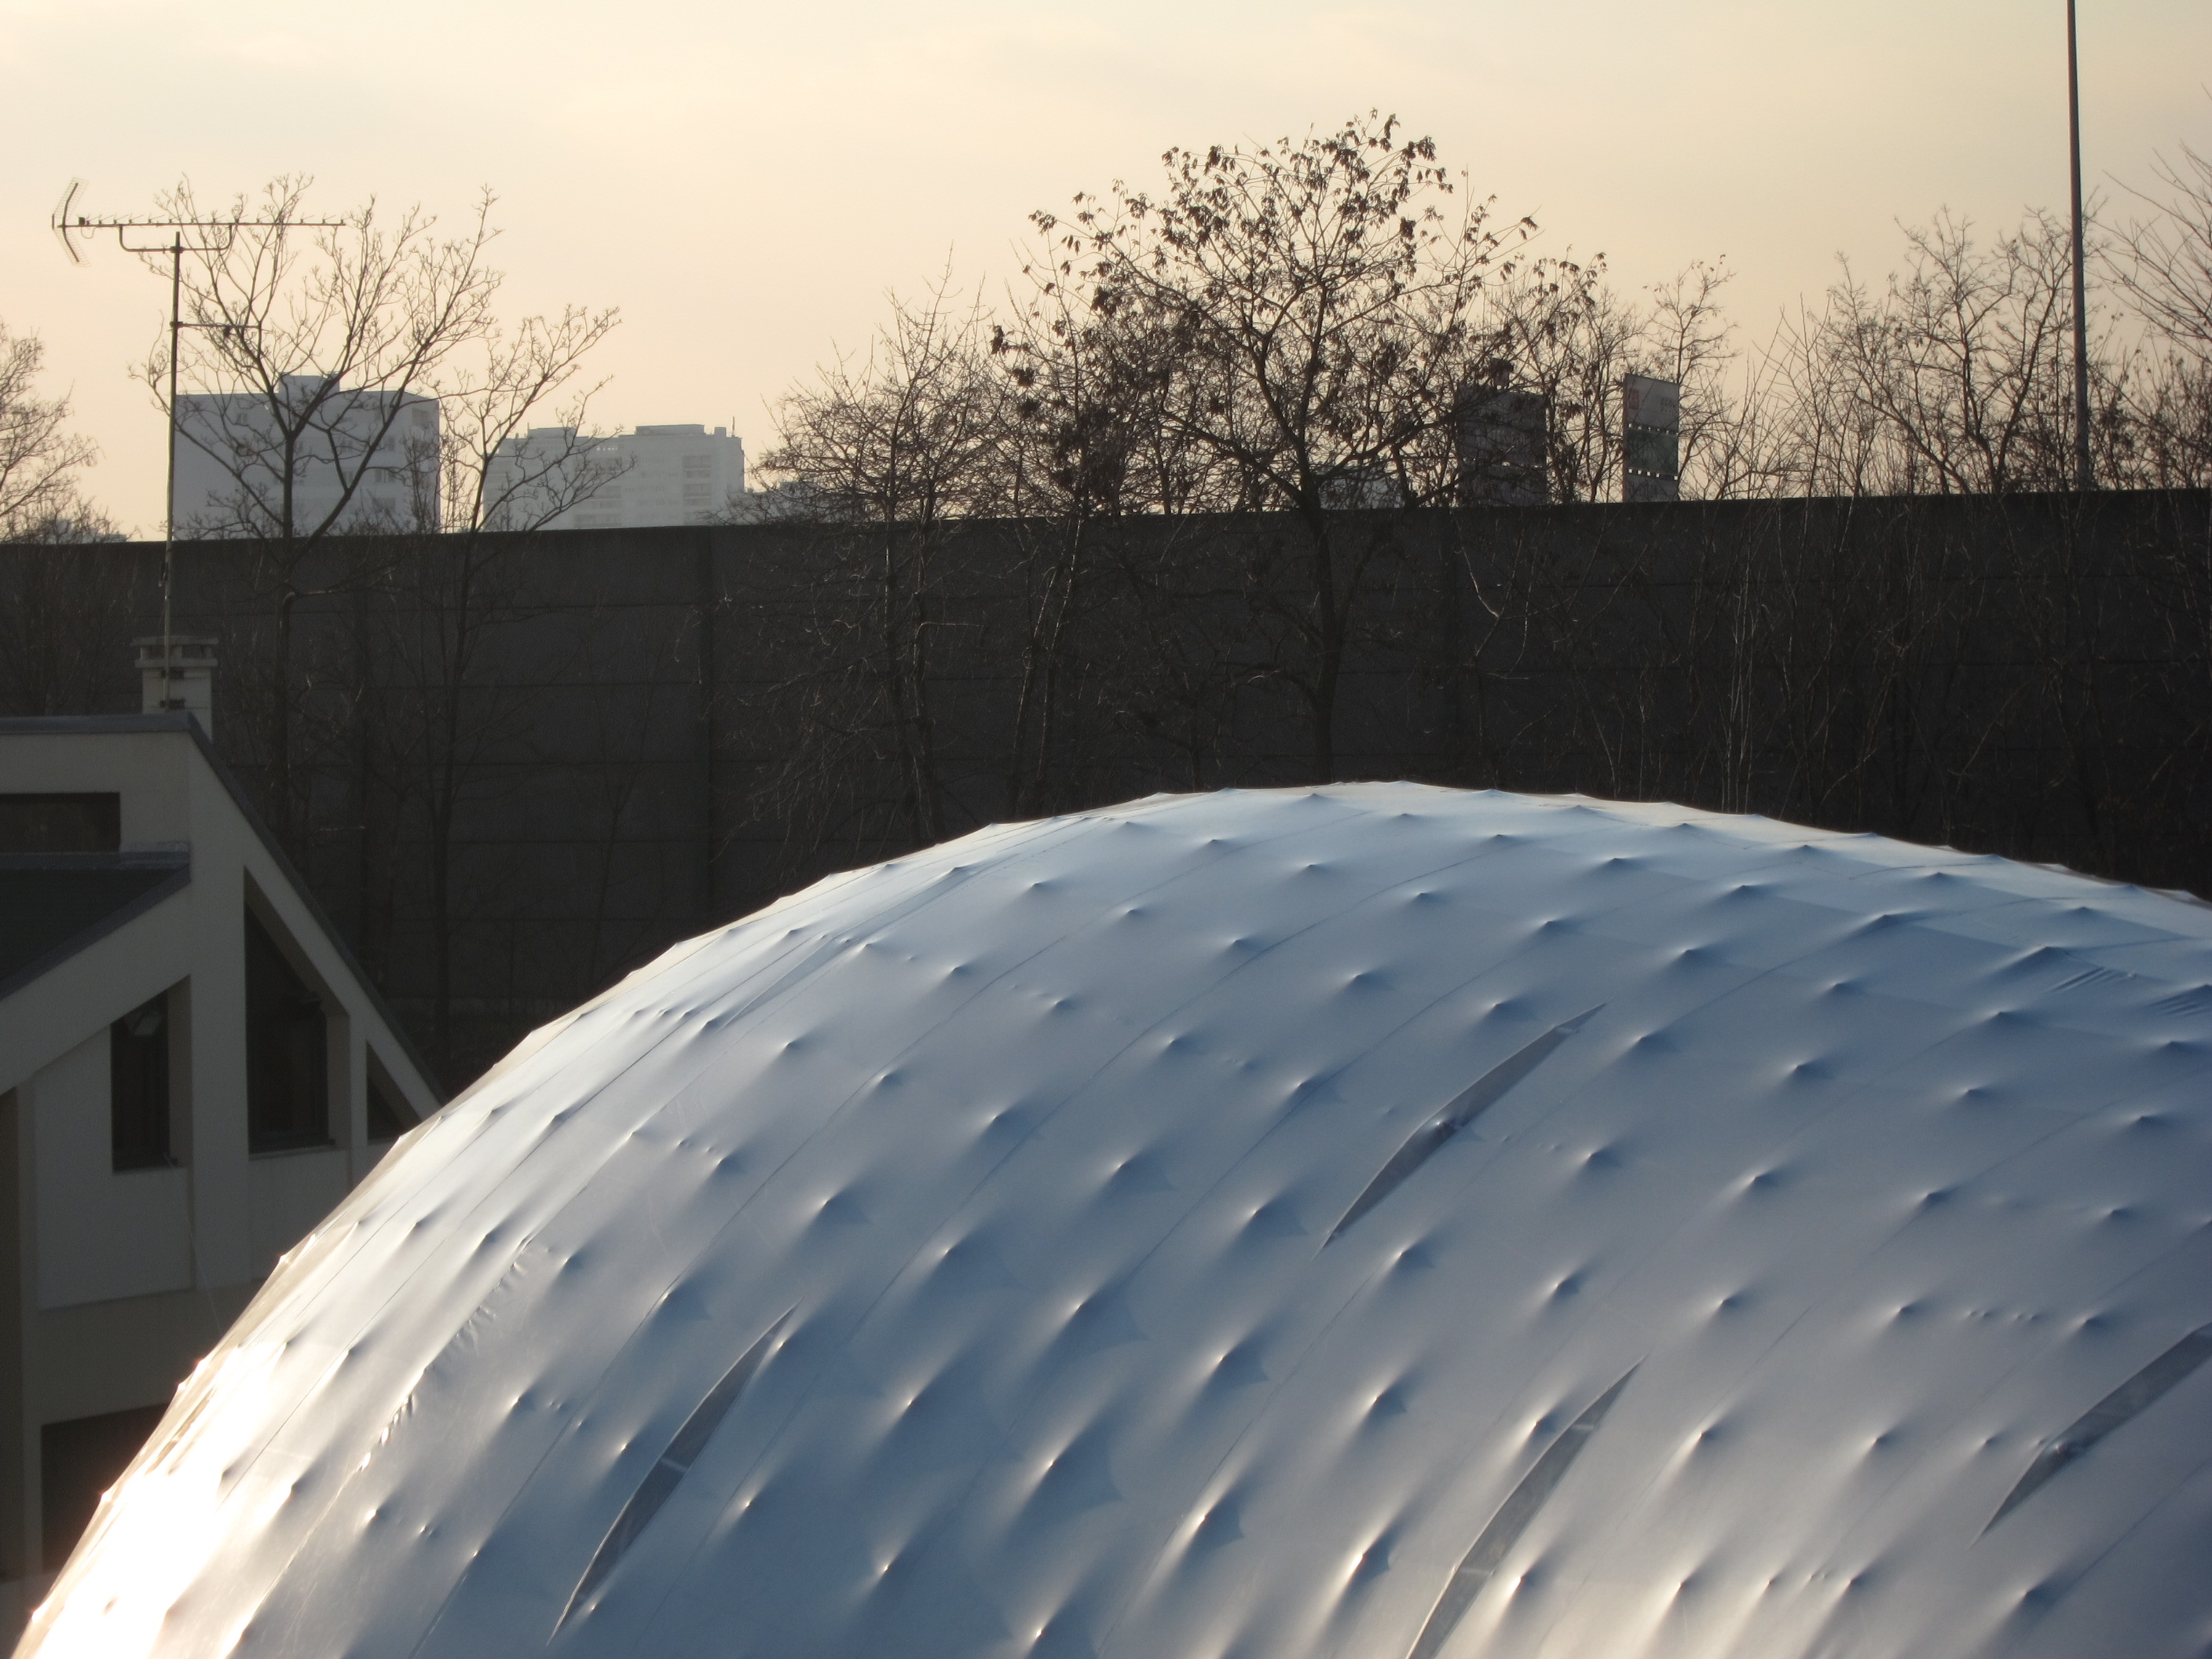
\includegraphics[width=\tmpwidth]{gs_ext}}
		\intersectnode{PPtl |- CAtl}{Pt}
		\Photo[
			node=Pt,
			anchor=north west,
			xshift=0mm,
			gopt={width=\tmpwidth},
			]{gs_ext.jpg}%
		\savenodes{A}
		\intersectnode{CAtl |- Abr}{Pt}
		\PhotoCaptionRef[
			hrefnode=Atl,
			node=Atr,
			anchor=south east,
			yshift=\PhotoRefSkip,
			phantom=true,
			]{figure}{}{Exterior view}{fig:gs_ext}
		\intersectnode{CAtl |- Abr}{Pt}
		\PhotoTextBox[
			node=CAbl,
			anchor=south west,
			% yshift=-\PhotoBigSkip,
			border=false,
			% width=4cm-\PhotoSkip,
			]{%
				\figurecaption[The connections mark the fabric suggesting the interior grid structure. This texture enriches the perception of the building viewed from the outside and creates effects with the light reflections.]{fig:gs_ext}
			}
	}
	\doubleblankpage[l]{%
		\hbox{}\thispagestyle{empty}
		\PhotoSpread[
			node=CAtl,
			anchor=north west,
			gopt={height=\textheight}
		]{gs_int.jpg}
		\AddToShipoutPictureBG*{
			\PhotoCaptionRef[
				hrefnode=TL,
				node=BL, 
				anchor=north west,
				yshift=-\PhotoRefSkip,
				phantom=true,
			]{figure}{}{Interior view}{fig:gs_int}}
	}{%
		\hbox{}\thispagestyle{empty}
		\AddToShipoutPictureBG*{
		\PhotoTextBox[
			node=BR,
			anchor=south west,
			xshift=\PhotoBigSkip,
			border=false,
			]{%
				\figurecaption[The grid pattern highlights the lightness of the structure and gives its tempo to the internal space. Lines converge to the altar, the heart of the liturgical area where the mass is offered on.]{fig:gs_int}
			}
	}}
}

\subsection{Daylight}
The gridshell is covered by a PVC membrane, which is opaque. How to introduce daylight into the interior was a major subject of reflection. The simplest way found was to use transparent membrane placed occasionally on the membrane. A small amount of light was required in the interior to create a contemplative atmosphere. The lights would in consequence glow and would be seen as luminous insertions in the vault, like stars in the celestial vault or the apse of some Romanesque churches. The stars were patterned on the joints of the PVC membrane. The almond shape came from simplification of the cutting into the panels either side of the joints and to avoid stress concentrations around cuts in the membrane. This shape, known as Mandela, is frequently used in Marian religious imagery. The distribution of the transparent insertions is quite uniform but gets denser above the pinnacle.

\enlargethispage{-4.5cm}
\AddToShipoutPictureBG*{% 
	\setlength{\tmpwidth}{\textwidth+\ContentInnerMargin+\BleedInnerMargin+\ContentBindingOffset}
	\settoheight{\tmpheight}{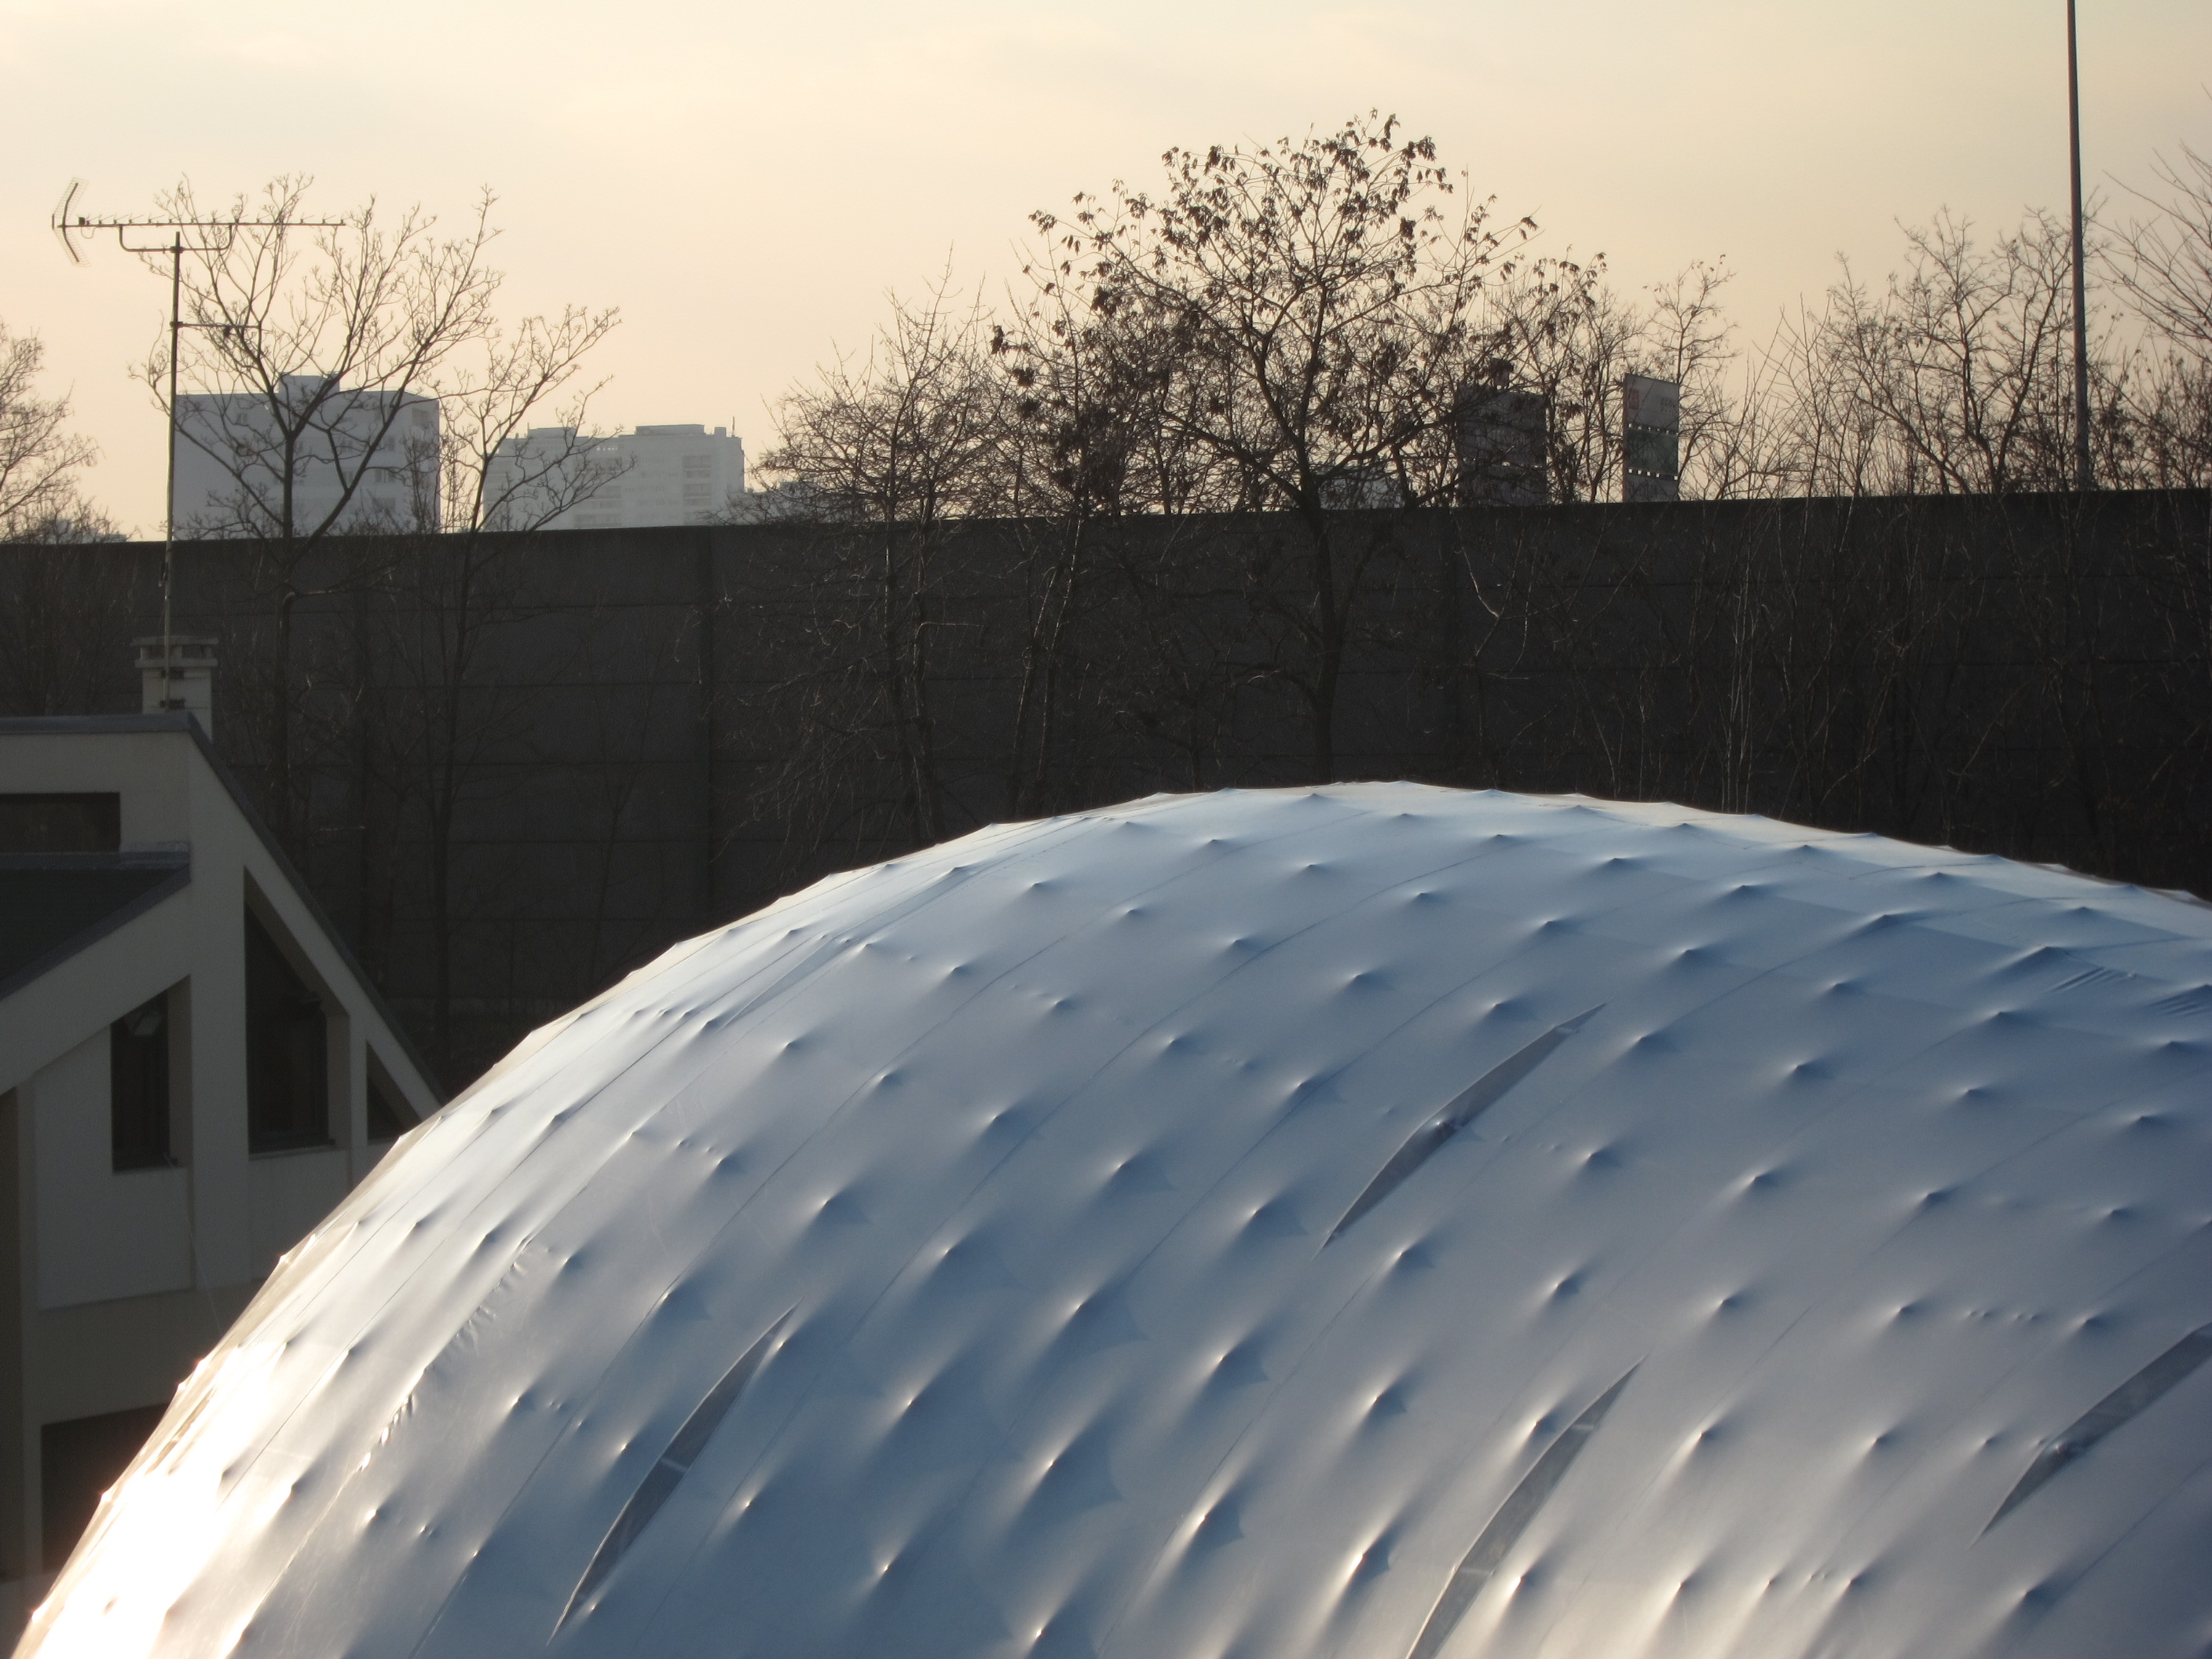
\includegraphics[height=4cm]{gs_ext}}
	\intersectnode{PPtl |- CAtl}{Pt}
	\Photo[
		node=CAbl,
		anchor=south west,
		gopt={height=4cm},
		]{door_ext.jpg}%
	\savenodes{A}
	\Photo[
		node=Atr,
		anchor=north west,
		xshift=\PhotoSkip,
		gopt={height=4cm},
		]{door_int.jpg}%
	\savenodes{B}
	\PhotoCaptionRef[
			node=Atl,
			anchor=north west,
			phantom=true;
			]{figure}{}{Steel doors}{fig:door}
		\PhotoCaptionRef[
			hrefnode=Atl,
			node=Atl,
			anchor=south west,
			yshift=\PhotoRefSkip,
			]{subfigure}{}{Interior view}{fig:door_int}
		\PhotoCaptionRef[
			hrefnode=Btl,
			node=Btl,
			anchor=south west,
			yshift=\PhotoRefSkip,
			]{subfigure}{}{Exterior view}{fig:door_ext}
	\PhotoTextBox[
		node=Bbr,
		anchor=south west,
		xshift=\PhotoSkip,
		border=false,
		width=4cm-\PhotoSkip,
		]{%
			\figurecaption[Two steel doors allow the entrance inside the building.]{fig:door}\par\bigskip
			\figurecaption{fig:door_int}\par
			\figurecaption{fig:door_ext}
		}
}

\subsection{Technical description}
% ------------------------------------------


\blankpage{%
	\thispagestyle{empty}
	\hbox{}
	\AddToShipoutPictureBG*{% 
		\def\tmpwidth{(\textwidth+\ContentOuterMargin+\BleedOuterMargin-\PhotoSkip)/2}
		\Photo[
			node=CAtl,
			anchor=north west,
			xshift=0mm,
			gopt={width=\tmpwidth},
			]{swivel.jpg}%
		\savenodes{A}
		\Photo[
			node=Atr,
			anchor=north west,
			xshift=\PhotoSkip,
			gopt={width=\tmpwidth},
			]{sleeve.jpg}%
		\savenodes{B}
		\Photo[
			node=Abl,
			anchor=north west,
			yshift=-\PhotoBigSkip,
			gopt={width=\tmpwidth},
			]{anchorage.jpg}%%
		\savenodes{C}
		\Photo[
			node=Bbl,
			anchor=north west,
			yshift=-\PhotoBigSkip,
			gopt={width=\tmpwidth},
			]{edge.jpg}%
		\savenodes{D}
		%%
		\PhotoCaptionRef[
			node=Atl,
			anchor=south west,
			yshift=-\PhotoSkip,
			phantom=true,
			]{figure}{}{Key elements of the structural system}{fig:parts}
		\PhotoCaptionRef[
			hrefnode=Atl,
			node=Atl, 
			anchor=south west, 
			yshift=\PhotoRefSkip,
			]{subfigure}{}{Swivel coupler}{fig:swivel}
		\PhotoCaptionRef[
			hrefnode=Btl,
			node=Btl, 
			anchor=south west, 
			yshift=\PhotoRefSkip,
			]{subfigure}{}{Sleeve system}{fig:sleeve}
		\PhotoCaptionRef[
			hrefnode=Ctl,
			node=Cbl, 
			anchor=north west, 
			yshift=-\PhotoRefSkip,
			]{subfigure}{}{Ground anchorage}{fig:anchorage}
		\PhotoCaptionRef[
			hrefnode=Dtl,
			node=Dbl, 
			anchor=north west, 
			yshift=-\PhotoRefSkip,
			]{subfigure}{}{Lacing rod}{fig:edge}
		\PhotoTextBox[
			node=CAbl,
			anchor=south west,
			width=10cm,
			border=false,
			]{%
				\figurecaption{fig:parts}\par
				\figurecaption{fig:swivel}\par
				\figurecaption{fig:sleeve}\par
				\figurecaption{fig:anchorage}\par
				\figurecaption{fig:edge}
			}
	}
}

The gridshell structure is made of long glass fibre tubes (\O 42~mm) fastened together with scaffold swivel couplers (see, \cref{fig:swivel}). The structural members of the grid, all of different lengths, are built  from one, two or three composite tubes connected with steel sleeves (see \cref{fig:sleeve}). The length of the tubes is limited to 12~m to enable transportation through standard trucks. The tubes are organized in three layers. During assembly, the first two layers are first placed perpendicular to one another on the ground. They form the \emph{quadrangular primary grid}. The distance between the tubes of these two layers is constant, resulting in a regular grid. This primary grid is elastically deformed to obtain the final shape. The third layer of tubes acts as bracing. It gives the structure a shell-like behavior. The tubes are fixed to the primary grid once the shape has been obtained.

The structure is anchored to a concrete strip footing with a special anchorage system, which ensures transfer of loads from the composite structure to the ground (see \cref{fig:anchorage}). A similar system enables fixation of the structure to the doors (see \cref{fig:door_int}).

A PVC coated fabric (see \cref{fig:gs_ext}), tailor-made for the purpose, covers the structure. The transparent portion of the structure allows daylight inside the gridshell. The fabric is stretched on the peripheral edge of a dedicated beam with a double-lacing system (halyard and strap, see \cref{fig:edge}). At the ground level, the lacing edge of the beam is made of a bent composite rod nailed to the concrete slab. At the grid–door junction, a steel arch is welded to the doorframe (see \cref{fig:door_ext}). The PVC fabric is waterproof and, since it is a continuous membrane, has no joints except at the perimeter. At the perimeter, a continuous strip of membrane is prefixed to the internal surface of the membrane and fixed to the ground slab. At the doors, a flexible strip of the membrane is riveted to the doorframe.

\blankpage{
	\hbox{}\thispagestyle{empty}
	\AddToShipoutPictureBG*{
		\SBox[%
			node=CAc,
			anchor=center,
			]{%
				% \ra{0.95}
				\begin{tabular}{@{}lllrr@{}}
					\toprule
					Category	 & Item 						& Unit 						& Quantity\\
					\midrule
					Public  	& seating  						& p							& 360 \\
								& standing 						& p							& 500 \\
					\midrule
				%	\addlinespace[0.5cm]
					Dimensions  &  length						& m 						& 29	\\
								&  width 						& m							& 17	\\
								&  height 						& m							& 7	\\
								& contour 	 					& lm						& 75\\
								& area							& m\textsuperscript{2}		& 350\\
								&  volume						& m\textsuperscript{3}		& 1600 \\
					\midrule
				%	\addlinespace[0.5cm]
					Gridshell   &  tubes (x176)					& lm						& 1775 \\
								&  connections					& 							& 1130 \\
								&  sleeves						& 							& 125 \\
								& anchorages 					& 							& 127 \\
								& \quad \emph{ground (single)} 	& 							& 77 \\
								& \quad \emph{ground (double)} 	& 							& 16 \\
								& \quad \emph{door (single)} 	& 							& 18 \\
								& weight  						& kg/m\textsuperscript{2} 	& 5 \\
					\midrule
				%	\addlinespace[0.5cm]
					Fabric   	& opaque						& m\textsuperscript{2}	 	& 530 \\
								& transparent					& m\textsuperscript{2}		& 12 \\
								& lacing rod					& lm 				 		& 67 \\
								& weight						& kg/m\textsuperscript{2}	& 1 \\
					\bottomrule
				\end{tabular}
			}
		\PhotoCaptionRef[
			node=CAtl, 
			anchor=north west, 
			% yshift=-\PhotoRefSkip,
			phantom=true,
			]{table}{}{Key figures}{tab:kfigures}
		\PhotoTextBox[
			node=CAbl,
			anchor=south west,
			border=false,
			]{\tablecaption{tab:kfigures}}
	}
}


\blankpage{
	\thispagestyle{empty}
	\hbox{}
	\AddToShipoutPictureBG*{% 
		\def\tmpwidth{\textwidth+\ContentOuterMargin+\BleedOuterMargin}
		\intersectnode{PPtl |- CAtl}{Pt}
		\Photo[
			node=Pt,
			anchor=north west,
			xshift=0mm,
			gopt={width=\PaperWidth},
			]{plan_view2}%
		\savenodes{A}
		\PhotoCaptionRef[
			node=Atl,
			anchor=south west,
			yshift=-\PhotoSkip,
			phantom=true,
			]{figure}{}{Top view of the building}{fig:plan_view}
		\PhotoTextBox[
			node=CAbl,
			anchor=south west,
			width=8cm,
			border=false,
			]{%
				\figurecaption[The interior space is composed of a choir (1), a place of assembly (2) and a narthex (3). The main entrance overlook the parvis (4). The shell spans about 29~m in the longitudinal direction and about 17~m in the transversal direction. The covered area is about 350~m\textsuperscript{2}. The space can accommodate 360 seating people or 500 standing people.]{fig:plan_view}\par
			}
	}

	\doubleblankpage{%
		\hbox{}\thispagestyle{empty}
		\intersectnode{PPtl |- CAbl}{Pt}
		\PhotoSpread[
			node=Pt,
			anchor=south west,
			yshift=-5cm,
			% lpcode={\thispagestyle{empty}},
			% rpcode={\thispagestyle{fancy}},
			gopt={width=2\PaperWidth}
		]{section_view2}
		\AddToShipoutPictureBG*{
			\PhotoCaptionRef[
				hrefnode=TL,
				node=BL, 
				anchor=north west,
				yshift=-\PhotoRefSkip,
				phantom=true,
			]{figure}{}{Transversal section of the building}{fig:sec}
			\PhotoTextBox[
				node=CAtl,
				anchor=north west,
				% xshift=\PhotoBigSkip,
				border=false,
			]{%
				\figurecaption[Observe how the grid gets denser at the choir. Two doors give access to the building. The height at the pinnacle is about 7~m.]{fig:sec}
			}
		}
	}{%
		\hbox{}\thispagestyle{empty}
		\AddToShipoutPictureBG*{
		\Photo[
			node=CAtr,
			anchor=north east,
			xshift=0mm,
			gopt={width=5cm},
			]{section_view_detail}%
		\savenodes{A}	
	}}
}



% \doubleblankpage[l]{
% 	\thispagestyle{empty}
% 	\hbox{}
% 	\AddToShipoutPictureBG*{% 
% 		\setlength{\tmpwidth}{\textwidth+\ContentInnerMargin+\BleedInnerMargin+\ContentBindingOffset}
% 		\intersectnode{PPtl |- CAbl}{Pt}
% 		\Photo[
% 			node=Pt,
% 			anchor=south west,
% 			% yshift=-\PhotoBigSkip,
% 			gopt={width=\tmpwidth},
% 			]{section_view}%
% 		\savenodes{B}
% 		\PhotoCaptionRef[
% 			node=Atl,
% 			anchor=south west,
% 			yshift=-\PhotoSkip,
% 			phantom=true,
% 			]{figure}{}{Transversal section of the building}{fig:sec}
% 		\PhotoTextBox[
% 			node=CAtl,
% 			anchor=north west,
% 			% width=10cm,
% 			border=false,
% 			]{%
% 				\figurecaption[Observe how the grid gets denser at the choir. Two doors give access to the building. The height at the pinnacle is about 7~m.]{fig:sec}
% 			}
% 	}
% }{%
% 	\thispagestyle{empty}
% 	\hbox{}
% }

% \begin{figure}[p]
% 	\captionsetup[subfloat]{captionskip=20pt}
%      	\centering
% 	\begin{fullpage}
% 		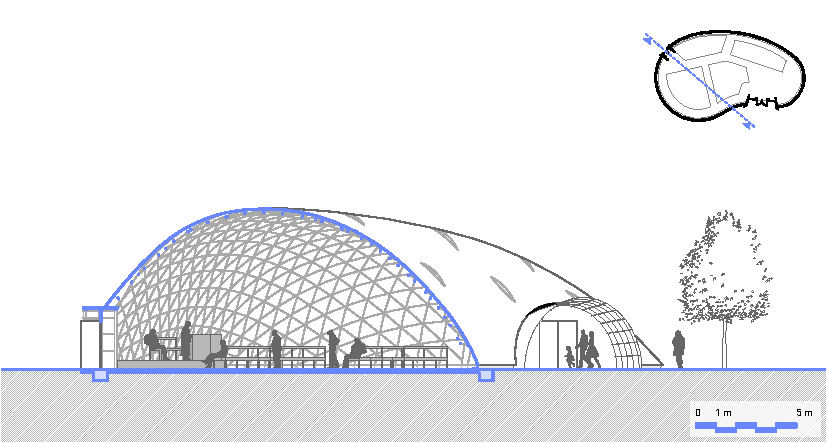
\includegraphics[width=\textwidth]{section_view}
% 		\caption[Transversal section of the building]{Transversal section of the building. Observe how the grid gets denser at the choir. Two doors give access to the building. The height at the pinnacle is about 7~m.}
% 		\label{fig:sec}
% 		%
% 		\vspace{1.5cm}
% 		%
% 		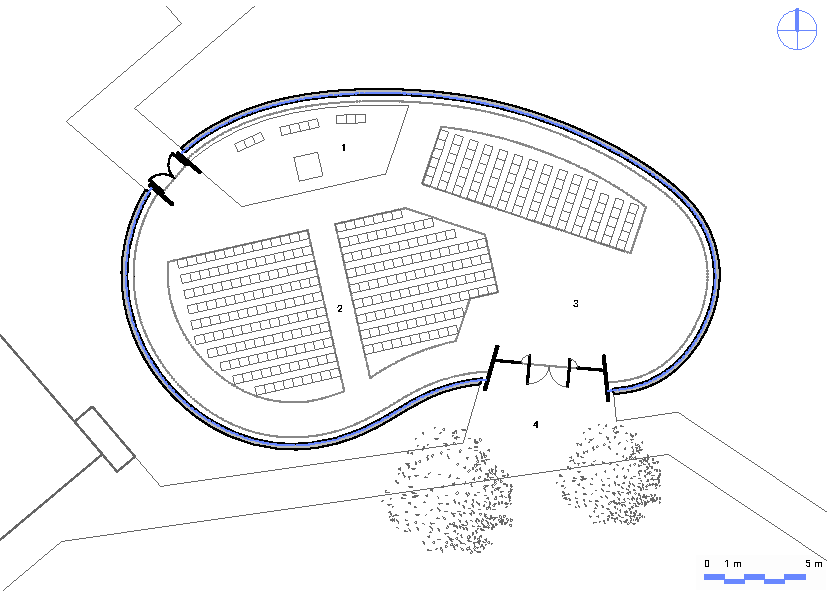
\includegraphics[width=\textwidth]{plan_view}
% 		\caption[Top view of the building]{Top view of the building. The interior space is composed of a choir (1), a place of assembly (2) and a narthex (3). The main entrance overlook the parvis (4). The shell spans about 29~m in the longitudinal direction and about 17~m in the transversal direction. The covered area is about 350~m\textsuperscript{2}. The space can accommodate 360 seating people or 500 standing people.}
% 		\label{fig:plan_view}
% 	\end{fullpage}
% \end{figure}


\pagebreak
\section{Construction process}\label{sec=construction_process}
% ====================

\subsection{Assembly of the grid}
The first two directions of tubes were assembled perpendicularly on the ground with the swivel couplers (see \cref{fig:swivel}) to form the \emph{primary} grid. The resulting grid covered about 600~m\textsuperscript{2} (see \cref{fig:cp_1}). At each intersection, the tubes were fastened together with a coupler, installed manually by the volunteers. They were asked not to tighten the bolts but just to engage the collars in order to prevent potential damages from the collar over the tube. Once the assembly of the primary grid was complet, the swivel couplers were tightened with a torque wrench to the optimal torque specified by the laboratoire Navier (F. Tayeb, J-F. Caron, L. du Peloux). The whole stage took two full days. Note that because the anchorages sticked out from the slab, it was decided not to assemble the grid on the concrete slab to ensure that the grid would be able to slide freely on the ground and not get clung in the anchorages during the erection stage.

\subsection{Deformation of the grid}
The next stage consisted in lifting the grid simultaneously with two mobile cranes (35t). Once lifted up, the grid took nearly its final form (see \cref{fig:cp_2}). The structure was slowly moved above the slab until tube endings faced at best their respective anchor points. Then, tube after tube, the workers pined the grid to the ground anchorages (see \cref{fig:cp_3}). This stage is tricky, especially at the beginning because only few tubes are connected to the ground. If the grid moves it can easily break these few tubes. The action of pinning a tube is done with a single bolt. The end of each composite tube is equipped with a rotating steel clevis. Similarly, each ground anchorage is composed of a steel plate fixed to the concrete slab and a rotating clevis. To pin a tube to an anchorage, their clevis are aligned one to each other and a pin is positioned in their central hole (see \cref{fig:anchorage}). When all the tubes were pinned to their anchorage, the grid was stable and secured and the cranes were removed (see \cref{fig:cp_4}). This stage lasted one full day.

\setlength{\tmpheight}{(\textheight-2\PhotoBigSkip)/3}
\intersectnode{PPtr |- CAtr}{Pt}
\PhotoSpread[
	node=Pt,
	anchor=north west,
	xshift=-2\PhotoBigSkip,
	gopt={height=\tmpheight},
	rpcode={\savenodes{AA}},
	]{erec_1a.jpg}%

\afterpage{
	\thispagestyle{empty}
	\hbox{\vspace{\textheight}}
	% \hbox{\vspace*{1cm}}
	\AddToShipoutPictureBG*{% 
		\intersectnode{PPtl |- CAtl}{Pt}
		% \def\tmpheight{(\textheight-2\PhotoBigSkip)/3}
		\Photo[
			node=AAtr,
			anchor=north west,
			xshift=\PhotoSkip,
			gopt={height=\tmpheight},
			]{erec_1b.jpg}%	
			\savenodes{AB}
		\intersectnode{CAtl |- AAtr}{Pt}
		\PhotoCaptionRef[
			hrefnode=CAtl,
			node=CAtl, 
			anchor=south west, 
			yshift=\PhotoRefSkip,
			phantom=true,
			]{figure}{}{Assembly of the grid}{fig:erec_1}
		\PhotoCaptionRef[
			hrefnode=CAtl,
			node=CAtl, 
			anchor=south west, 
			yshift=\PhotoRefSkip,
		]{subfigure}{}{GFRP tubes with swivel couplers}{fig:erec_1a}
		\PhotoCaptionRef[
			hrefnode=ABtl,
			node=ABtl, 
			anchor=south west, 
			yshift=\PhotoRefSkip,
			]{subfigure}{}{Primary grid}{fig:erec_1b}
	}
	\PhotoSpread[
		node=ABtr,
		anchor=north west,
		xshift=\PhotoWidth+\PhotoBigSkip,
		gopt={height=\tmpheight},
		]{erec_1c.jpg}%
	% \savenodes{AC}
	\AddToShipoutPictureBG*{%
		\PhotoCaptionRef[
			hrefnode=PStl,
			node=PStl, 
			anchor=south west, 
			yshift=\PhotoRefSkip,
			]{subfigure}{}{Cranes ready to lift the grid}{fig:erec_1c}
		\intersectnode{PPtl |- AAbr}{Pt}
		\Photo[
			node=Pt,
			anchor=north west,
			% xshift=\PhotoSkip,
			yshift=-\PhotoBigSkip,
			gopt={height=\tmpheight},
			]{erec_2a.jpg}%	
			\savenodes{BA}
		\Photo[
			node=BAtr,
			anchor=north west,
			xshift=\PhotoSkip,
			% yshift=-\PhotoBigSkip,
			gopt={height=\tmpheight},
			]{erec_2b.jpg}%	
			\savenodes{BB}
		\Photo[
			node=BAbl,
			anchor=north west,
			xshift=2\PhotoBigSkip,
			yshift=-\PhotoBigSkip,
			gopt={height=\tmpheight},
			]{erec_3a.jpg}%
		\savenodes{BC}
		%%
		\intersectnode{CAtl |- BBtr}{Pt}
		\PhotoCaptionRef[
			hrefnode=Pt,
			node=Pt, 
			anchor=south west, 
			yshift=\PhotoRefSkip,
			phantom=true,
			]{figure}{}{Deformation of the grid}{fig:erec_2}
		\PhotoCaptionRef[
			hrefnode=Pt,
			node=Pt, 
			anchor=south west, 
			yshift=\PhotoRefSkip,
		]{subfigure}{}{GFRP tubes with swivel couplers}{fig:erec_2a}
		\PhotoCaptionRef[
			hrefnode=BBtl,
			node=BBtl, 
			anchor=south west, 
			yshift=\PhotoRefSkip,
			]{subfigure}{}{Primary grid}{fig:erec_2b}
		\intersectnode{CAtl |- BCtr}{Pt}
		\PhotoCaptionRef[
			hrefnode=Pt,
			node=Pt, 
			anchor=south west, 
			yshift=\PhotoRefSkip,
			]{subfigure}{}{Primary grid}{fig:erec_2c}
		\PhotoTextBox[
			node=BCbr,
			anchor=south west,
			xshift=\PhotoBigSkip,
			width=10cm,
			border=false,
			]{%
				\figurecaption{fig:erec_1}\par
				\figurecaption{fig:erec_1a}\par
				\figurecaption{fig:erec_1b}\par
				\figurecaption{fig:erec_1c}\par\medskip
				\figurecaption{fig:erec_2}\par
				\figurecaption{fig:erec_2a}\par
				\figurecaption{fig:erec_2b}\par
				\figurecaption{fig:erec_2c}
			}
	}
	%%
	\blankpage{%
		\thispagestyle{empty}
		\hbox{}
		\AddToShipoutPictureBG*{% 
			\intersectnode{PGtl |- AAbr}{Pt}
			\Photo[
				node=Pt,
				anchor=north west,
				xshift=2\PhotoBigSkip,
				yshift=-\PhotoBigSkip,
				gopt={height=\tmpheight},
				]{erec_4a.jpg}%
			\savenodes{DA}
			\Photo[
				node=DAtr,
				anchor=north west,
				xshift=\PhotoSkip,
				% yshift=-\PhotoBigSkip,
				gopt={height=\tmpheight},
				]{erec_4b.jpg}%
			\savenodes{DB}
			%%
			\intersectnode{PPtl |- DBbr}{Pt}
			\Photo[
				node=Pt,
				anchor=north west,
				% xshift=2\PhotoBigSkip,
				yshift=-\PhotoBigSkip,
				gopt={height=\tmpheight},
				]{erec_5a.jpg}%
			\savenodes{EA}
			\Photo[
				node=EAtr,
				anchor=north west,
				xshift=\PhotoSkip,
				% yshift=-\PhotoBigSkip,
				gopt={height=\tmpheight},
				]{erec_5b.jpg}%
			\savenodes{EB}
			\Photo[
				node=EBtr,
				anchor=north west,
				xshift=\PhotoSkip,
				% yshift=-\PhotoBigSkip,
				gopt={height=\tmpheight},
				]{erec_5c.jpg}%
			\savenodes{EC}
			%%%%
			\intersectnode{CAtl |- BBtr}{Pt}
			\PhotoCaptionRef[
				hrefnode=DAtl,
				node=DAtl, 
				anchor=south west, 
				yshift=\PhotoRefSkip,
				phantom=true,
				]{figure}{}{Deformation of the grid}{fig:erec_3}
			\PhotoCaptionRef[
				hrefnode=DAtl,
				node=DAtl, 
				anchor=south west, 
				yshift=\PhotoRefSkip,
			]{subfigure}{}{GFRP tubes with swivel couplers}{fig:erec_3a}
			\PhotoCaptionRef[
				hrefnode=DBtl,
				node=DBtl, 
				anchor=south west, 
				yshift=\PhotoRefSkip,
				]{subfigure}{}{Primary grid}{fig:erec_3b}
			%%%
			\intersectnode{DAtl |- EAtr}{Pt}
			\PhotoCaptionRef[
				hrefnode=Pt,
				node=Pt, 
				anchor=south west, 
				yshift=\PhotoRefSkip,
				phantom=true,
				]{figure}{}{Deformation of the grid}{fig:erec_4}
			\PhotoCaptionRef[
				hrefnode=Pt,
				node=Pt, 
				anchor=south west, 
				yshift=\PhotoRefSkip,
			]{subfigure}{}{GFRP tubes with swivel couplers}{fig:erec_4a}
			\PhotoCaptionRef[
				hrefnode=EBtl,
				node=EBtl, 
				anchor=south west, 
				yshift=\PhotoRefSkip,
				]{subfigure}{}{Primary grid}{fig:erec_4b}
			\PhotoCaptionRef[
				hrefnode=ECtl,
				node=ECtl, 
				anchor=south west, 
				yshift=\PhotoRefSkip,
				]{subfigure}{}{Primary grid}{fig:erec_4c}
			\PhotoTextBox[
				node=AAtr,
				anchor=north west,
				xshift=\PhotoBigSkip,
				width=10cm,
				border=false,
				]{%
					\figurecaption{fig:erec_3}\par
					\figurecaption{fig:erec_3a}\par
					\figurecaption{fig:erec_3b}\par\medskip
					\figurecaption{fig:erec_4}\par
					\figurecaption{fig:erec_4a}\par
					\figurecaption{fig:erec_4b}\par
					\figurecaption{fig:erec_4c}
				}
		}
	}
}

\subsection{Bracing of the grid}
Once the primary grid was deformed into the final shape, it was braced by a third direction of tubes called the \emph{triangulation}. The triangulation tubes split the quadrangular mesh of the primary grid into triangles (see \cref{fig:cp_5}). This work was tedious as it required working at height in aerial buckets. Tubes were hand-conveyed in the structure and attached to the tubes of the second layer with an additional swivel coupler. Each node of the structure would then be composed of two connections (see \cref{fig:swivel_dwg}). Once triangulated the structure behaves like a shell and its stiffness increases largely.




% \begin{figure}[p]
% 	%
%      	\centering
% 	\begin{fullpage}
% 		\subfloat[][Flat grid]{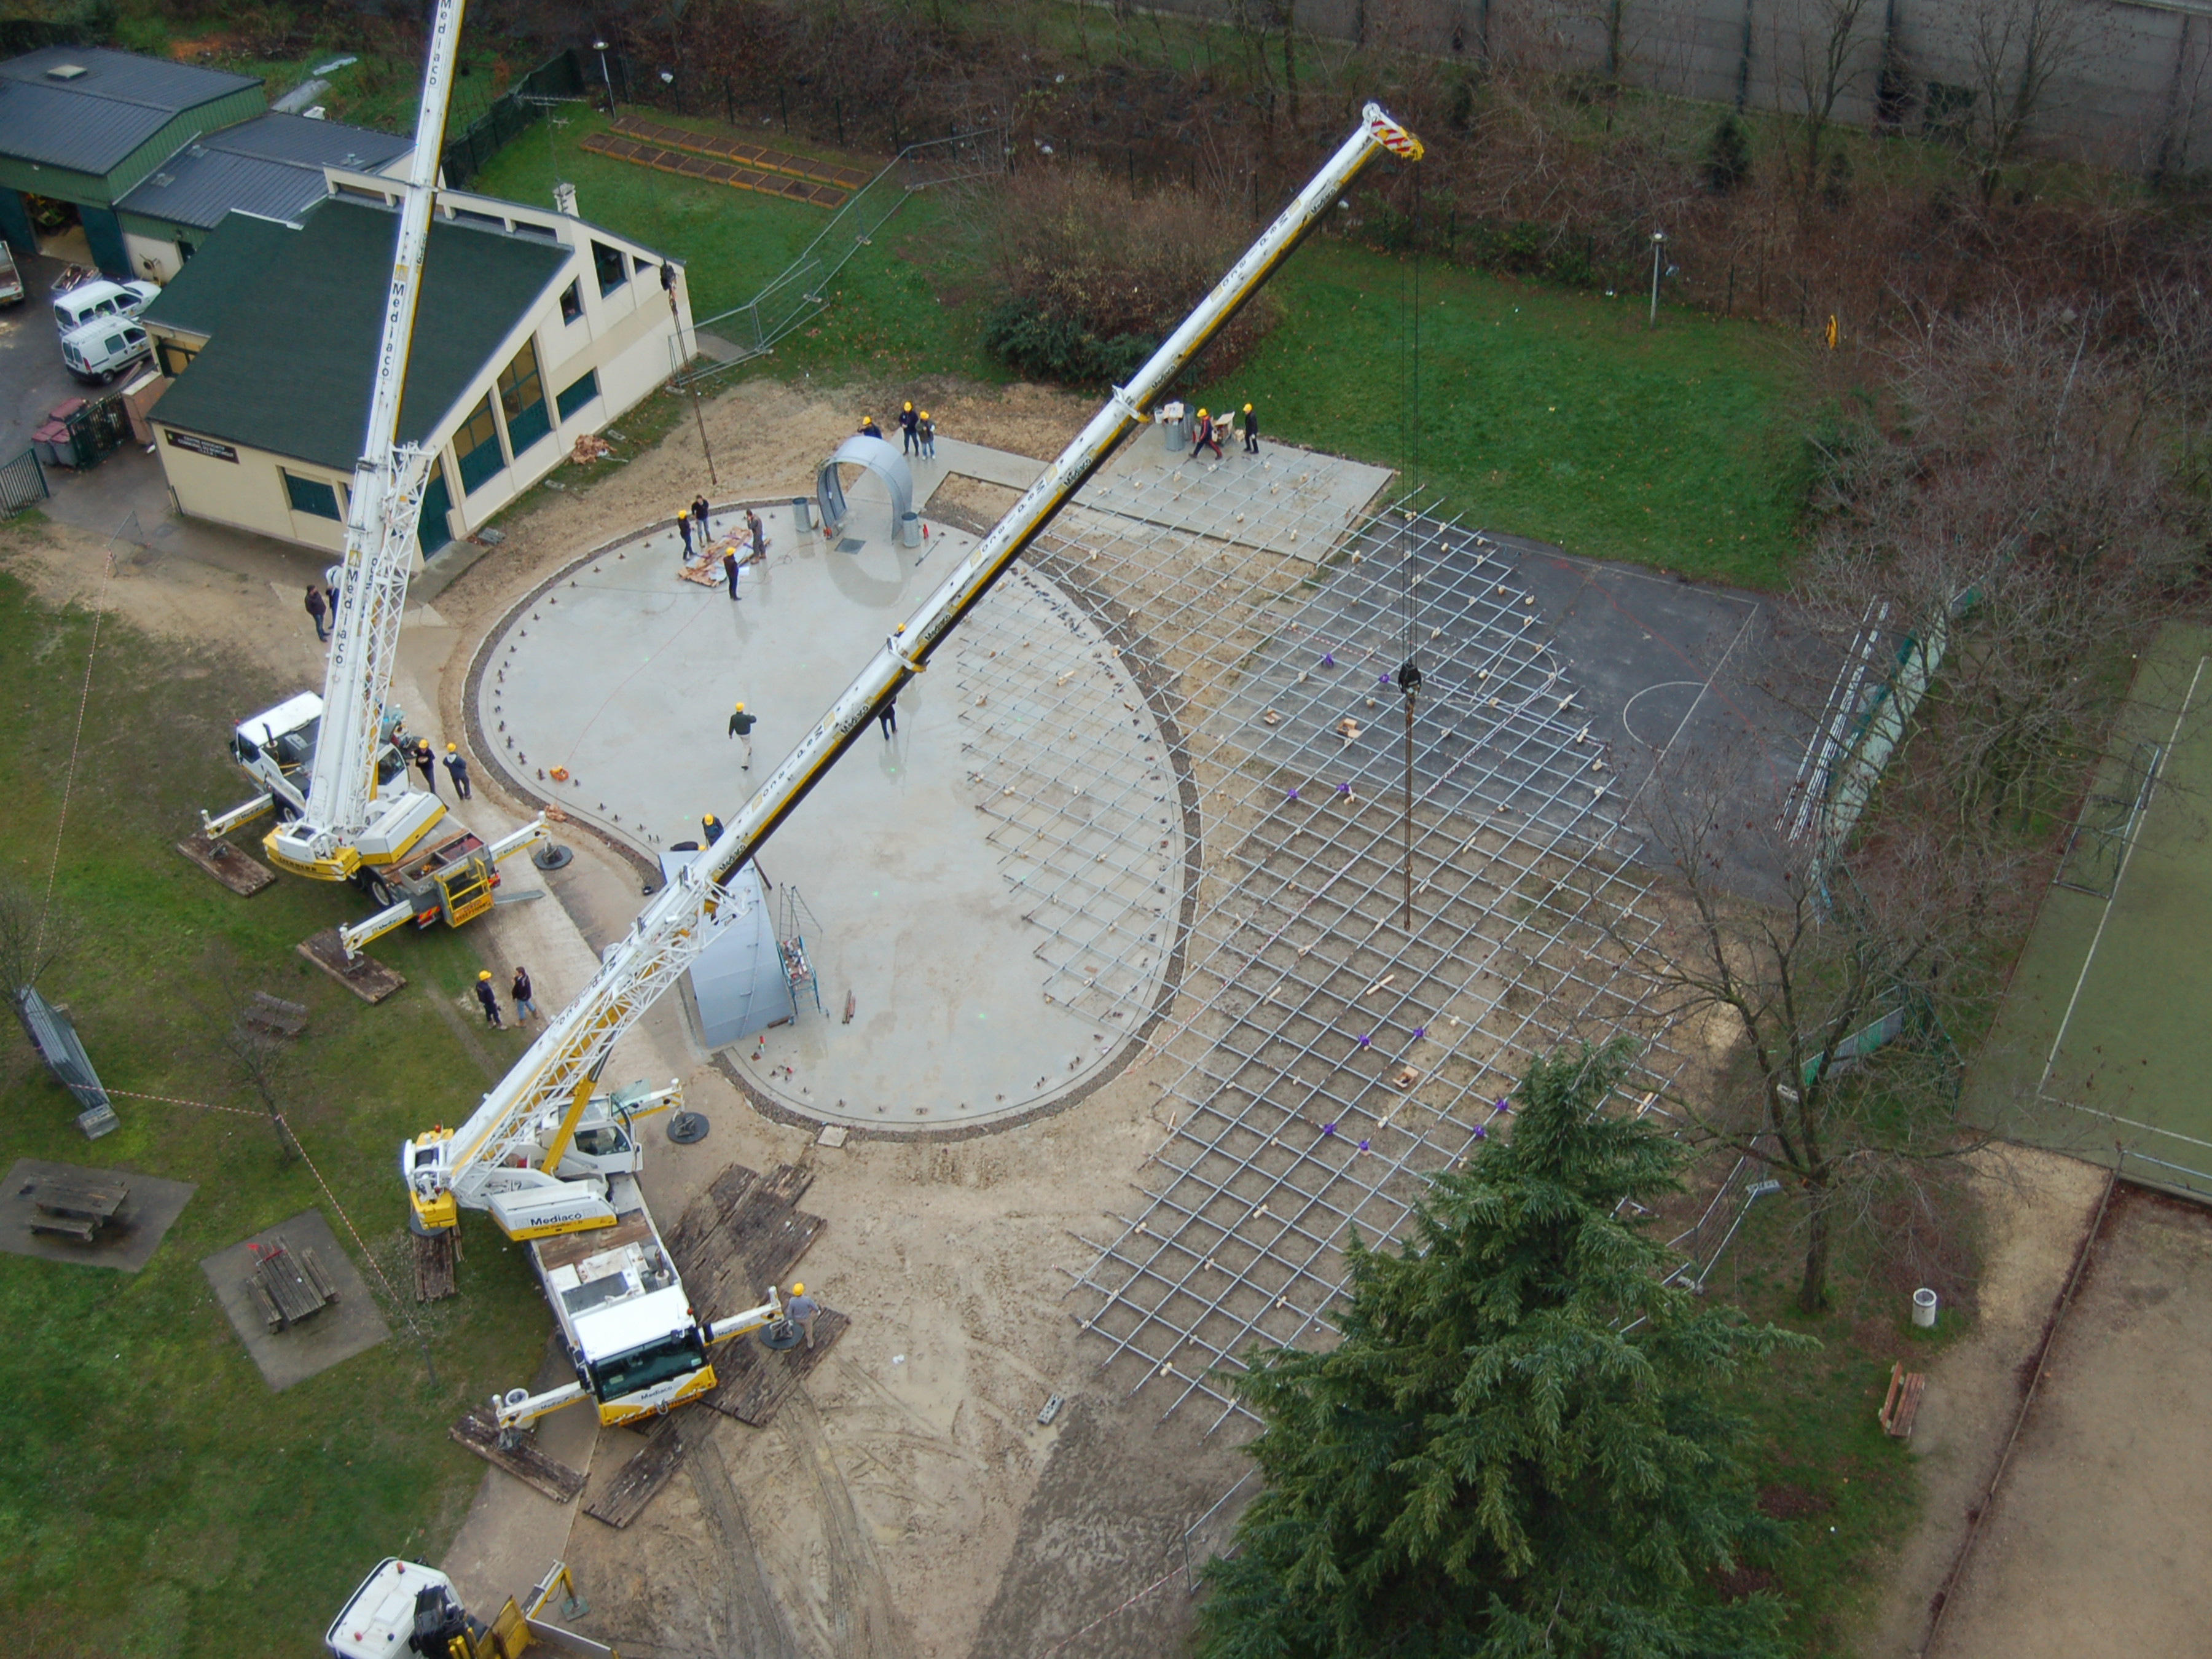
\includegraphics[width=0.48\textwidth]{cp_1.jpg}\label{fig:cp_1}}
% 		\hspace*{\fill}
% 		\subfloat[][Erection]{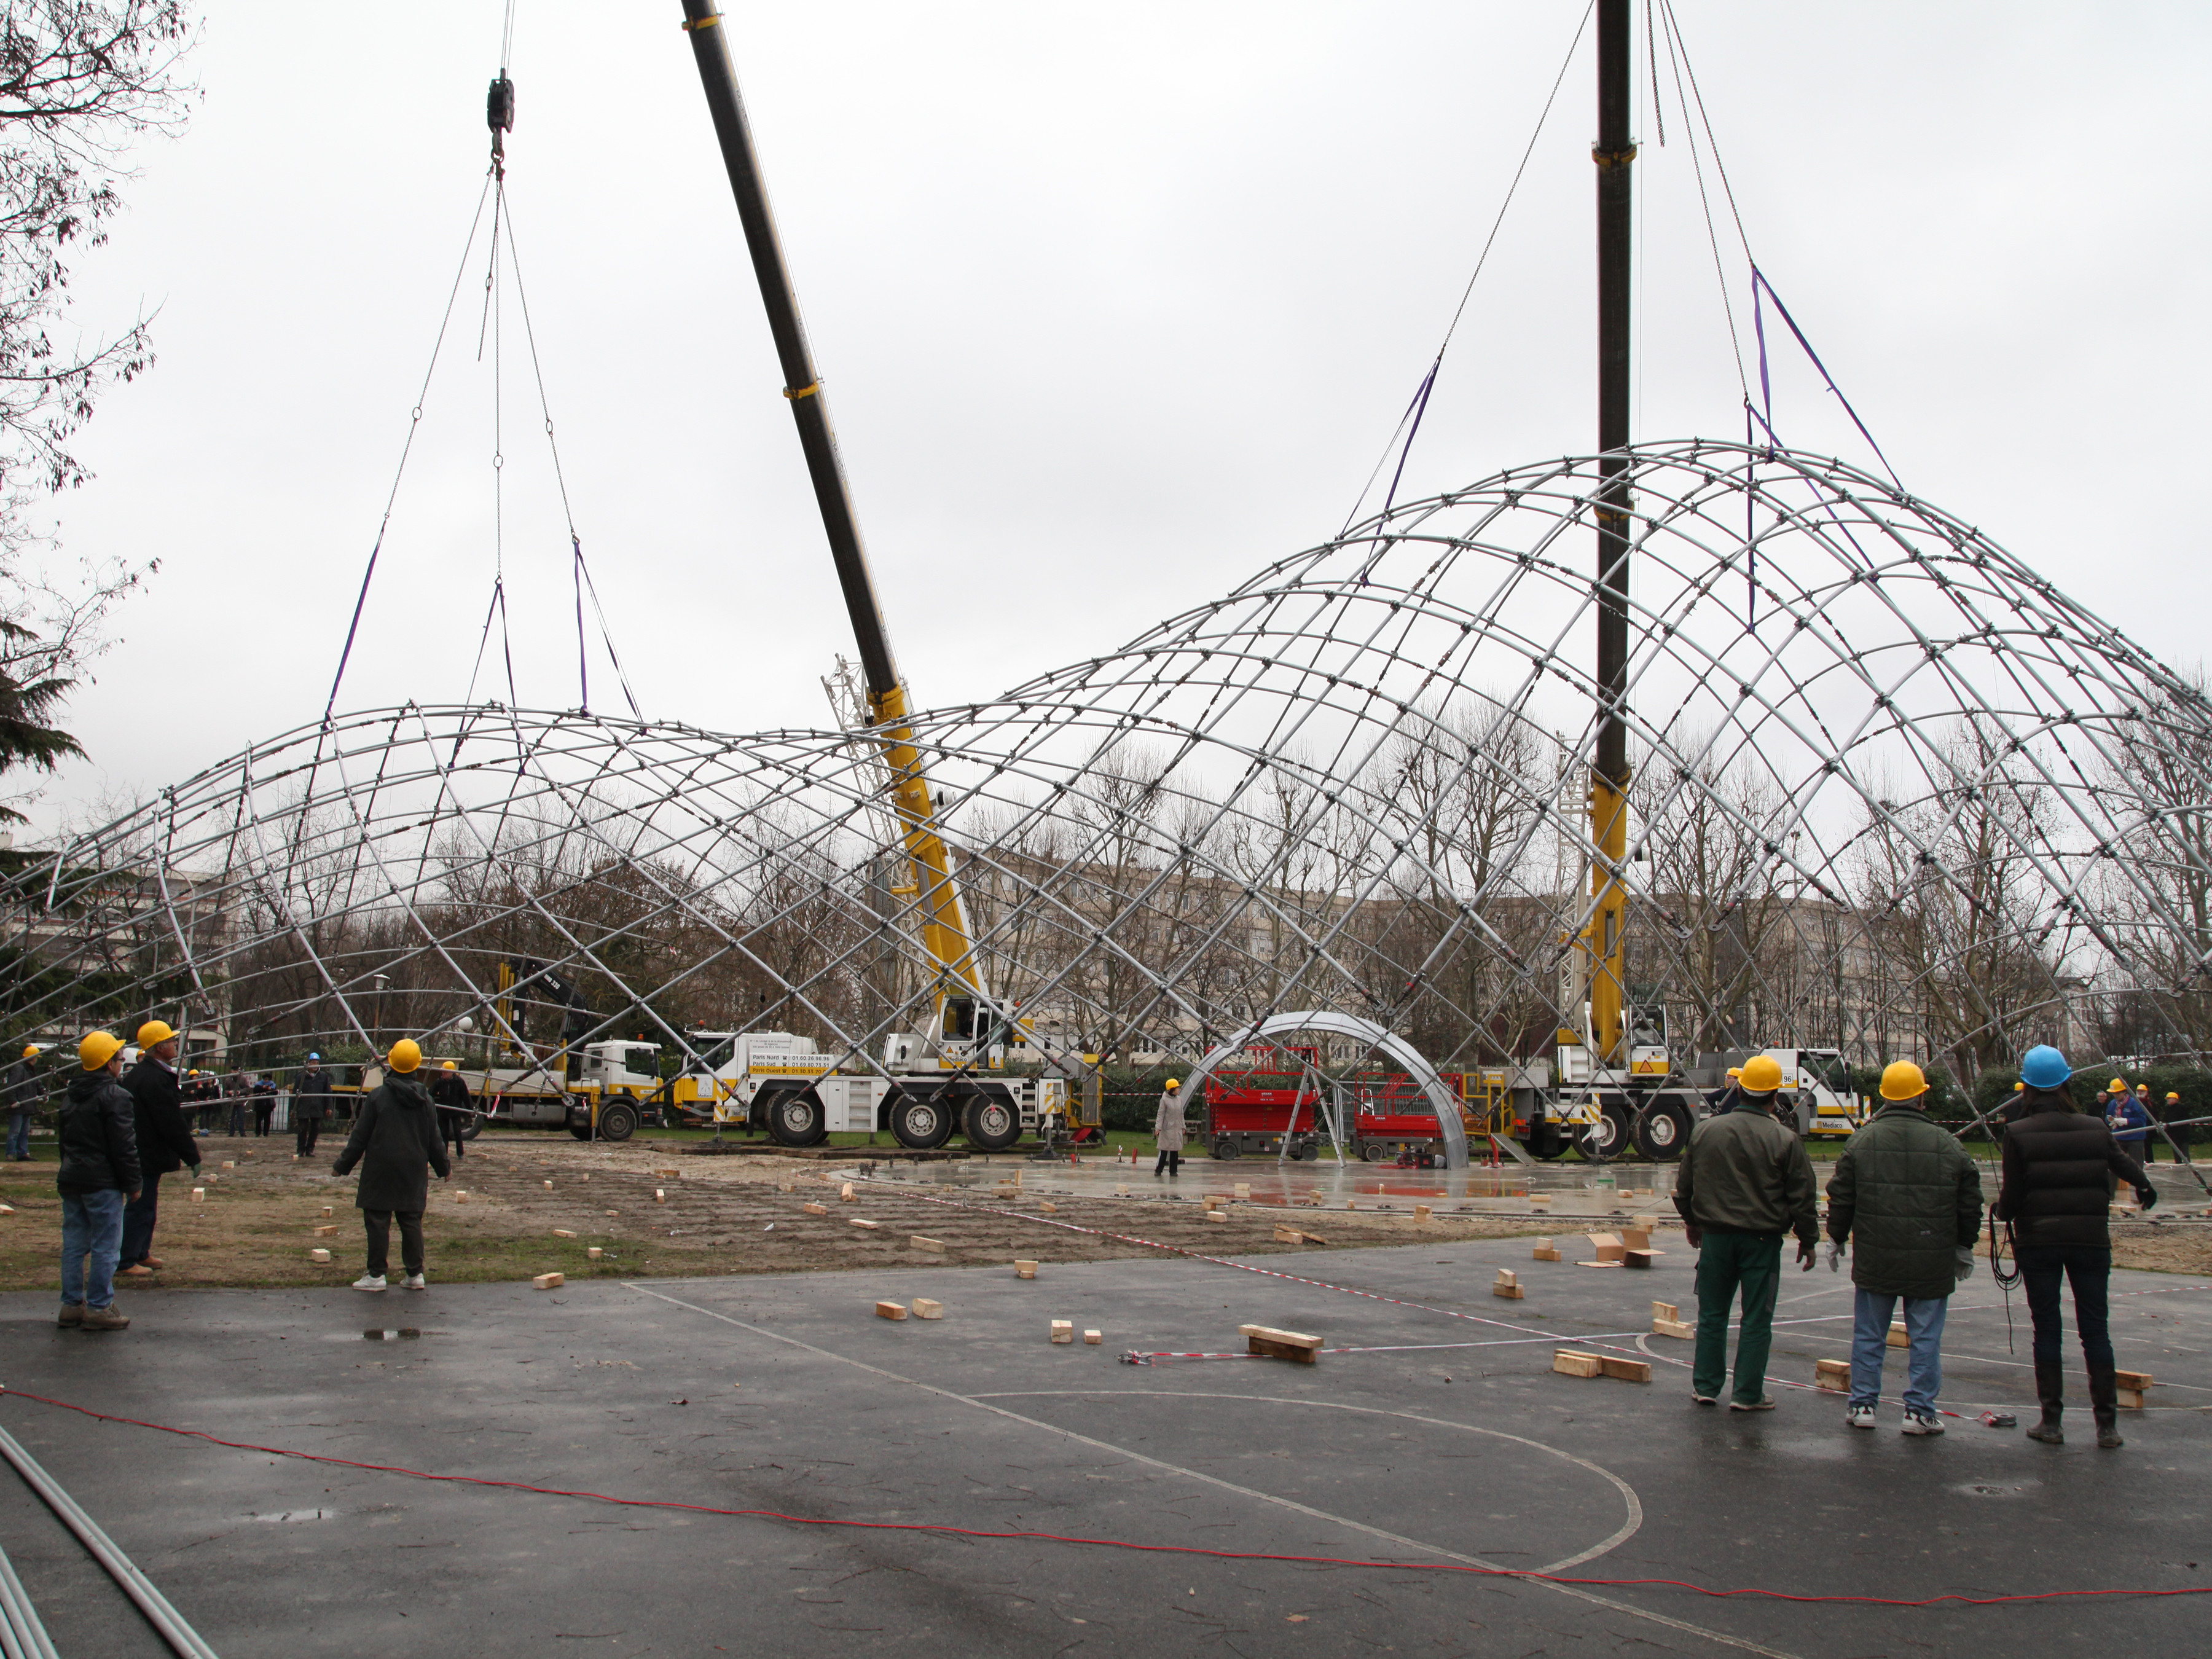
\includegraphics[width=0.48\textwidth]{cp_2.jpg}\label{fig:cp_2}} \\
% 		%
% 		\subfloat[][The grid is anchored]{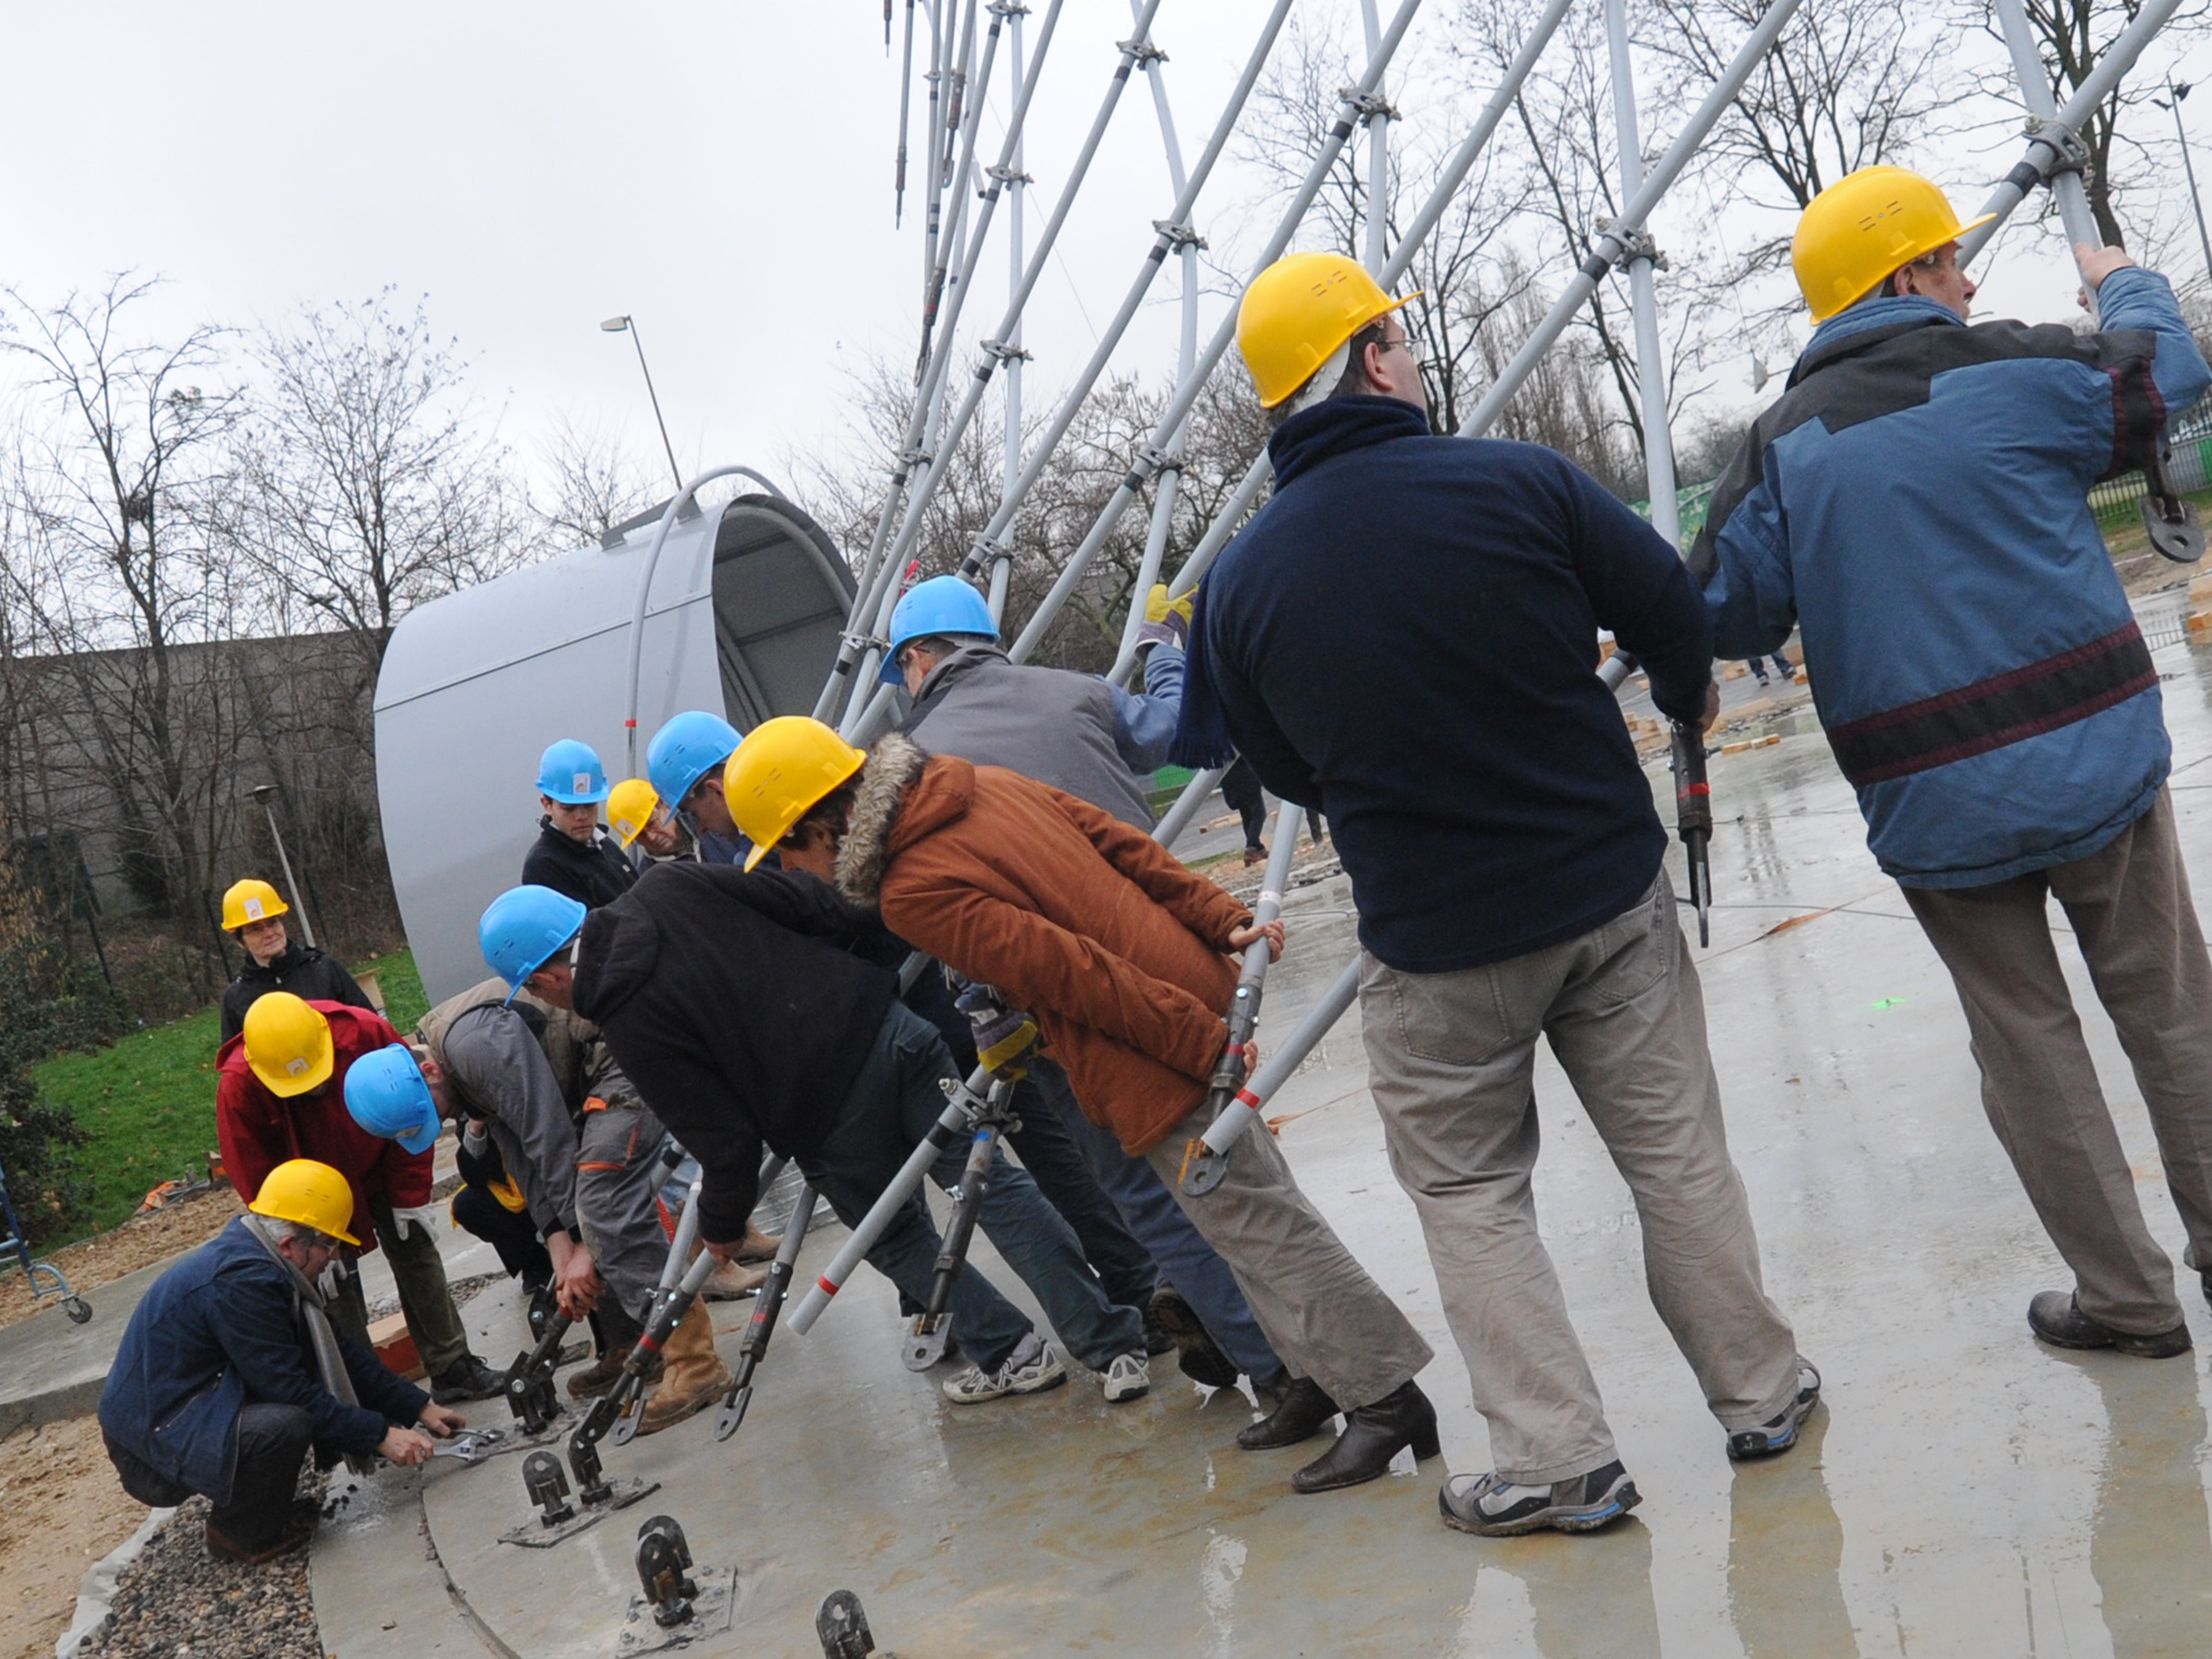
\includegraphics[width=0.48\textwidth]{cp_3.jpg}\label{fig:cp_3}}
% 		\hspace*{\fill}
% 		\subfloat[][Deformed grid]{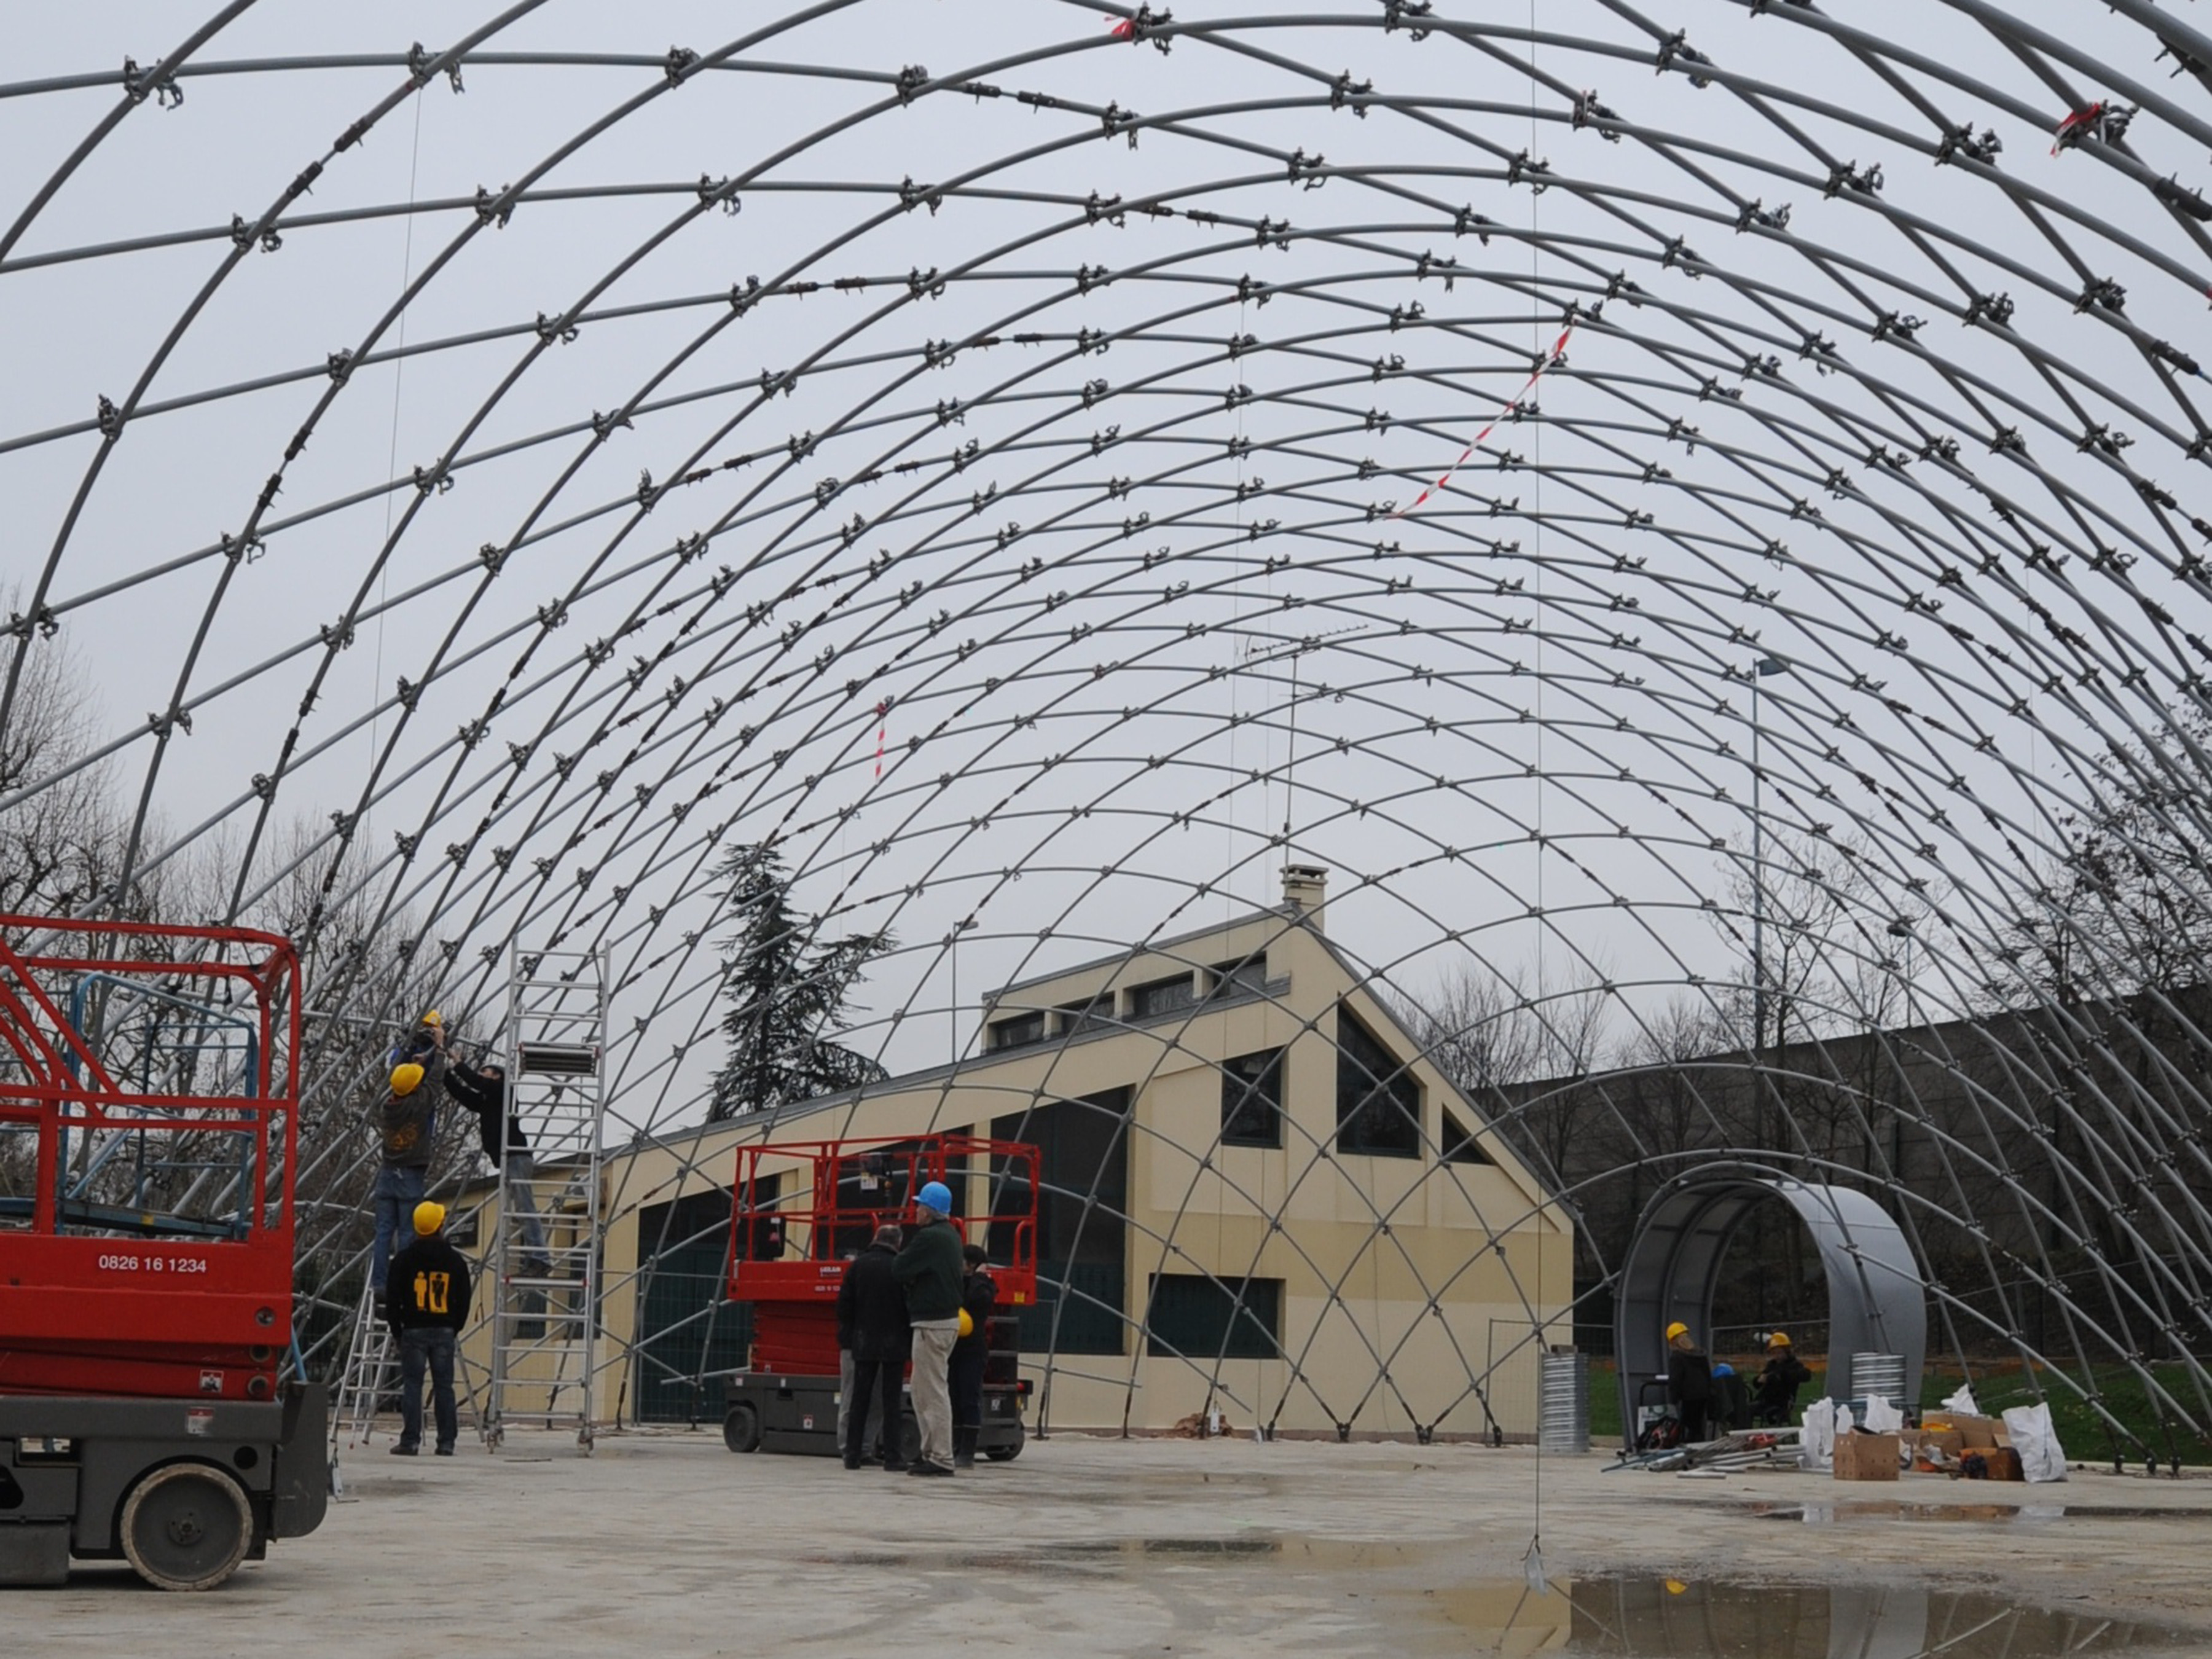
\includegraphics[width=0.48\textwidth]{cp_4.jpg}\label{fig:cp_4}} \\
% 		%
% 		\subfloat[][Grid is braced]{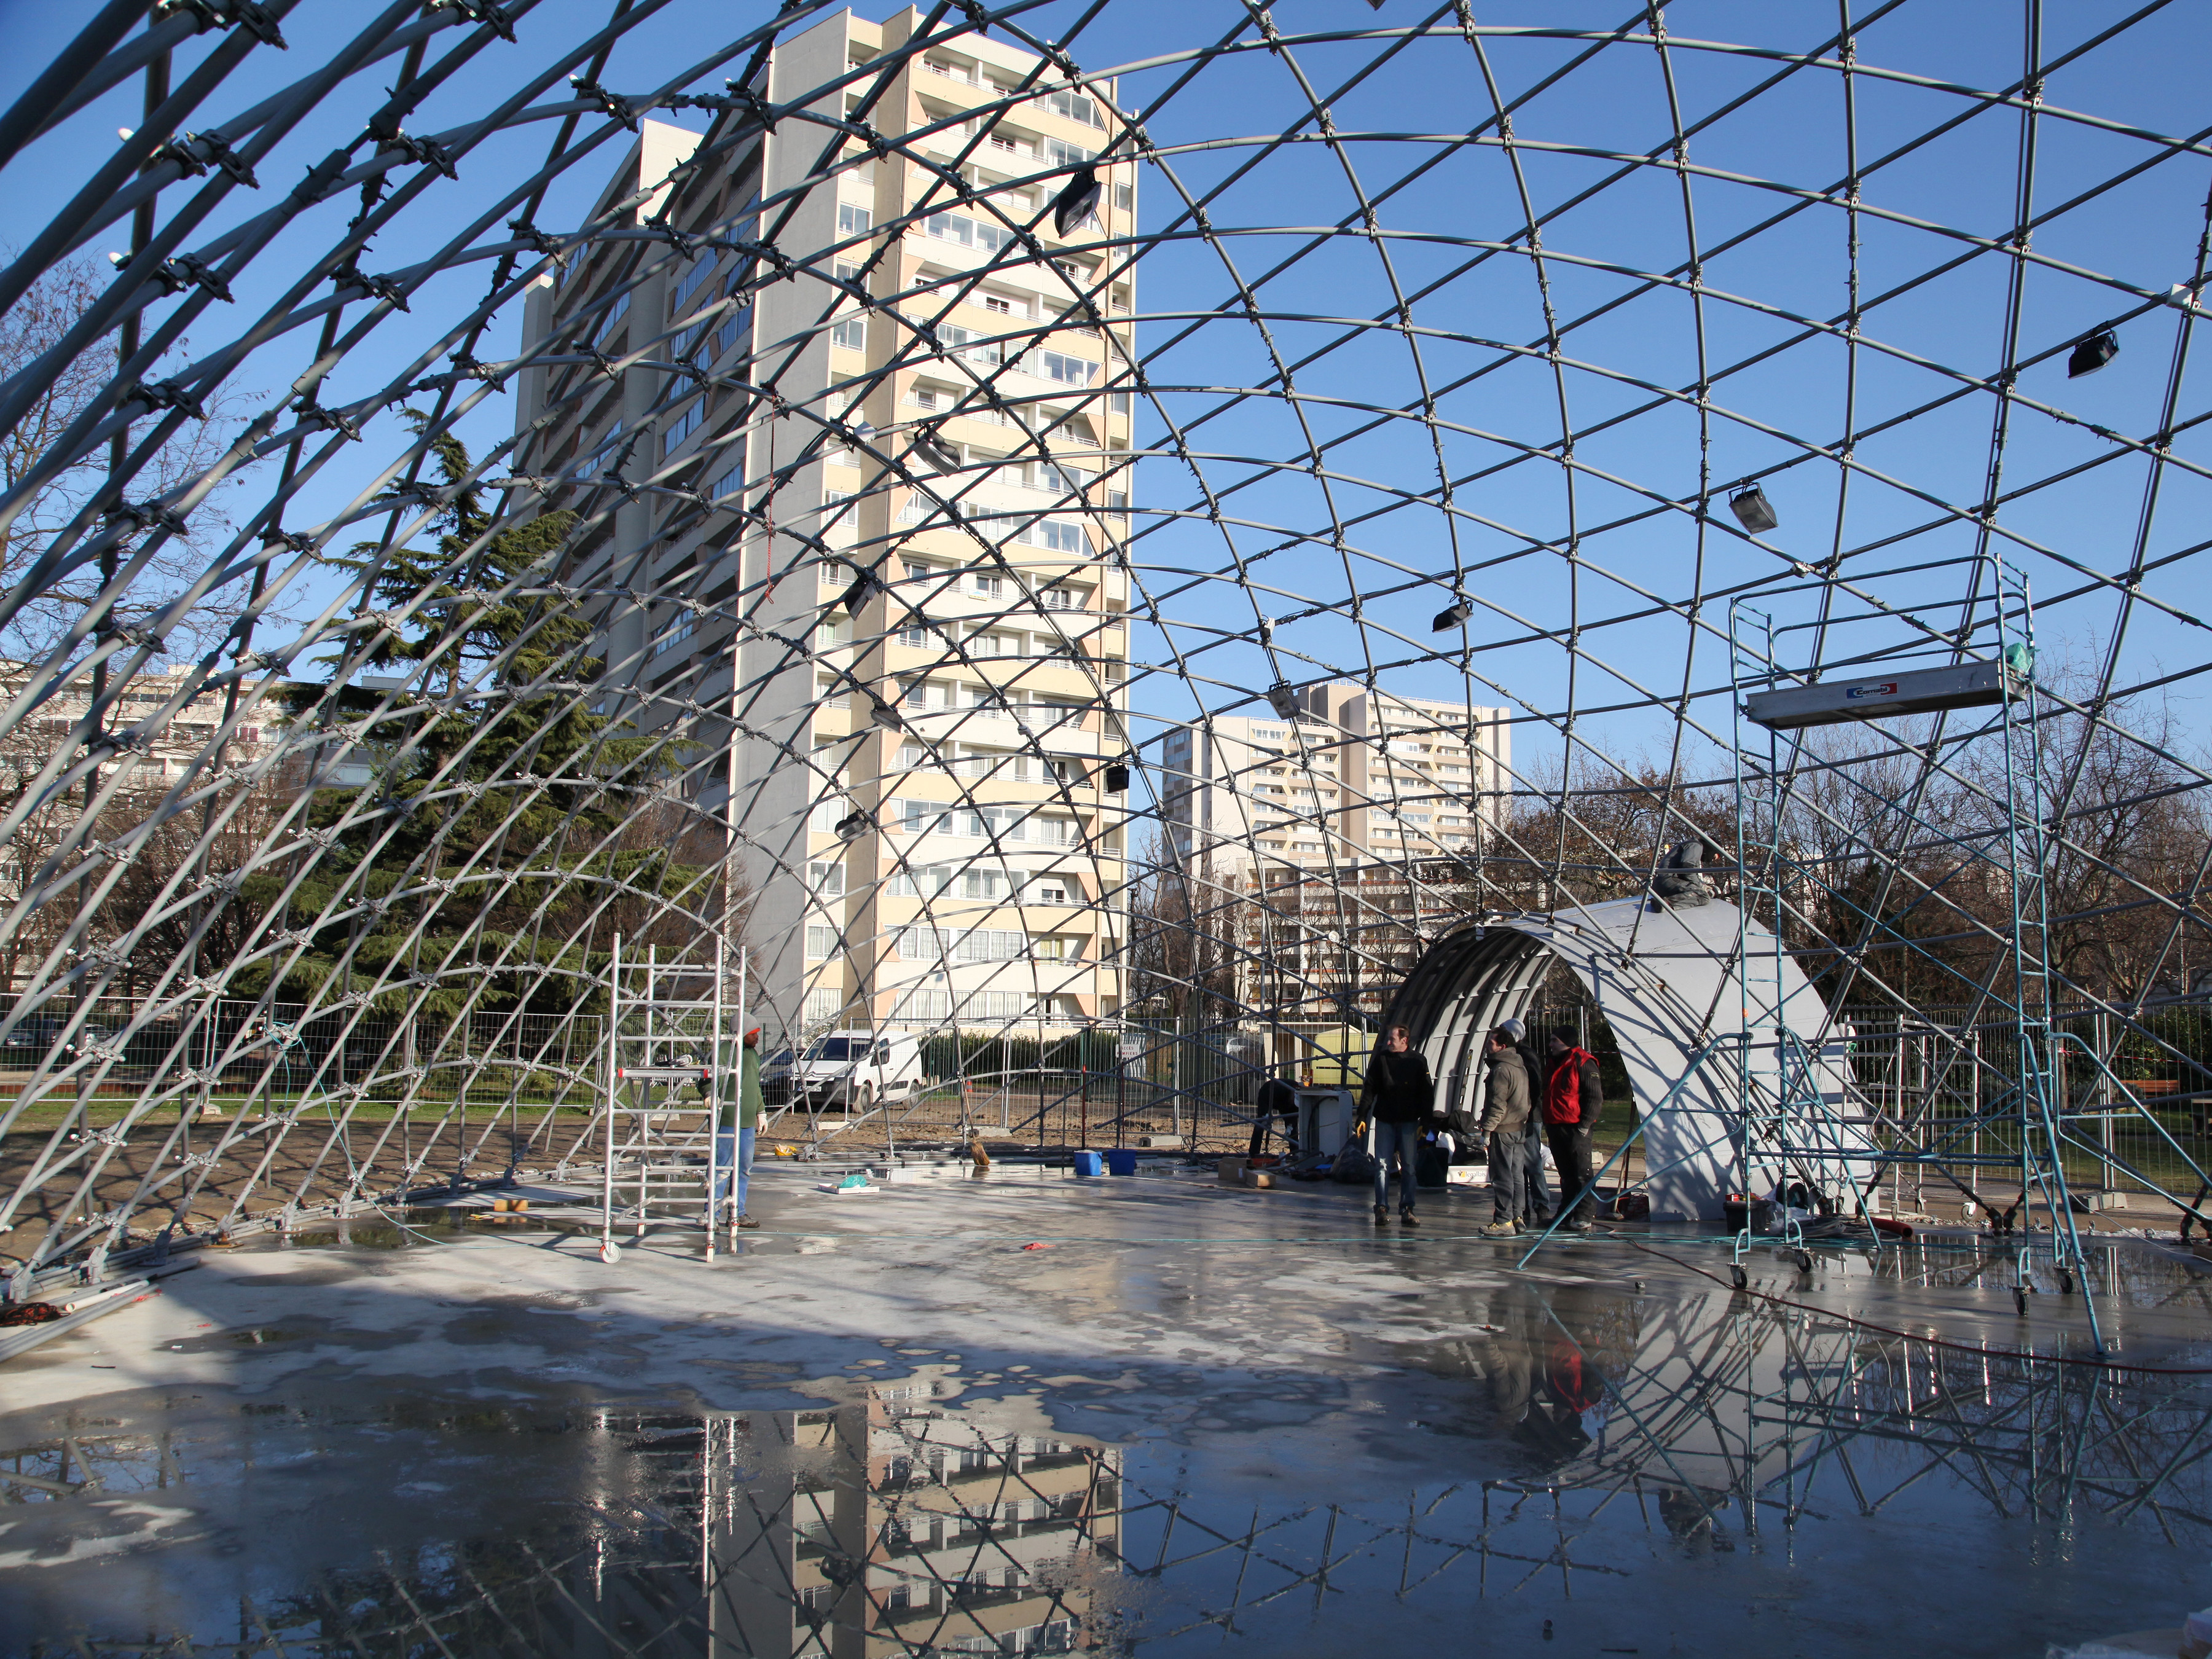
\includegraphics[width=0.48\textwidth]{cp_5.jpg}\label{fig:cp_5}}
% 		\hspace*{\fill}
% 		\subfloat[][Membrane]{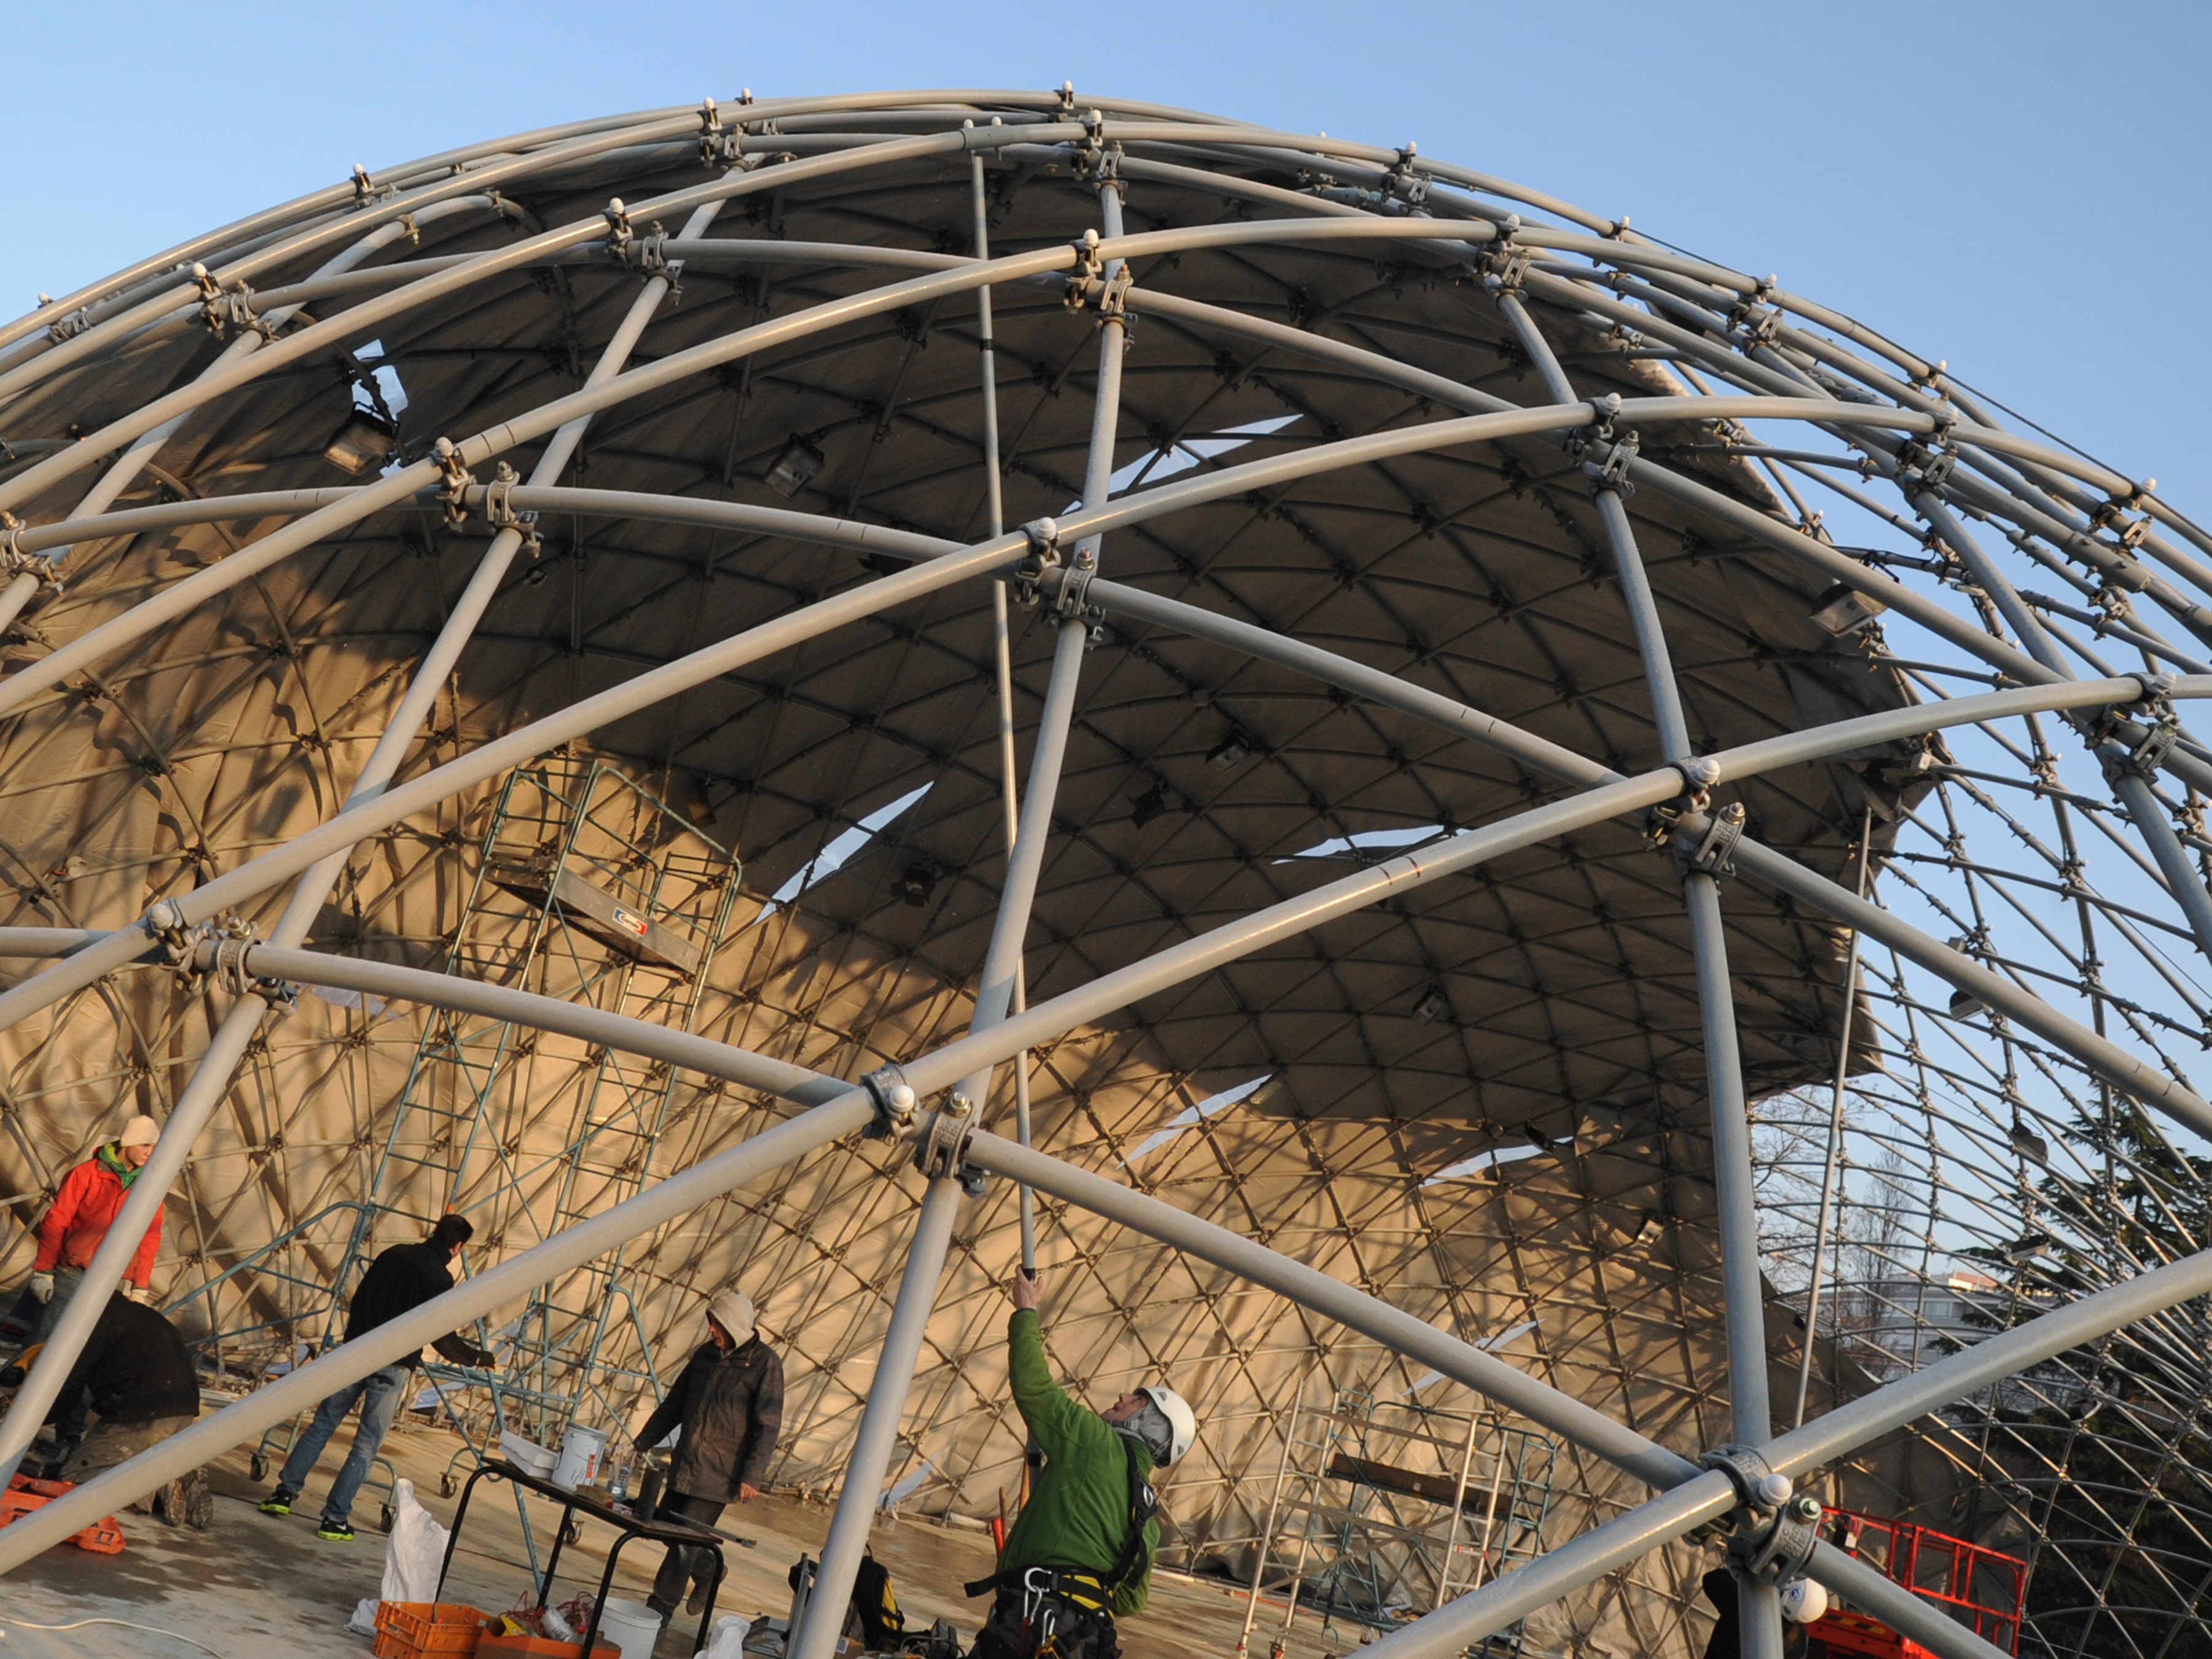
\includegraphics[width=0.48\textwidth]{cp_6.jpg}\label{fig:cp_6}} \\
% 		%
% 		\vspace{10pt}
% 		\caption{Construction process of the gridshell.}
% 		\label{fig:erection}
% 	\end{fullpage}
% \end{figure}

\subsection{Covering of the gridshell}
Finally, the structure is covered with a PVC coated fabric. The membrane comes rolled up. The roll is positioned at one side. Then it is progressively unrolled toward the other side (see \cref{fig:cp_6}). This step requires professional rope workers. Once the membrane is in place, it is hand tensioned with a system of halyard and strap (see \cref{fig:edge}). All included, this stage lasted no more than a single day for a team of six workers.

This step appears as the moment of truth~: if the membrane perfectly fits the gridshell, making no crease, that means the structural analysis was successfully conducted with the required accuracy (see \cref{sec=form-finding}).

%\clearpage
\section{Structural design}\label{sec=proj_design}
%=================

In this section, we exhibit a methodology to design a gridshell with a shape-centered approach. This is one of the key originality of this work and it was first implemented for the Solidays gridshell in 2011. The idea is to identify a grid and a set of supports that once the grid is bended and anchored to its foundations has a geometry as close as possible to the target shape designed by the architect.

Solving this inverse problem is quite a challenge. It requires a lot of back-and-forth between architects and engineers about the definition of the shape. To build a suitable solution the designers need agile tools to get deep insights quickly and adapt their design iteratively until convergence is reached. Unfortunately, existing structural analysis softwares are more validation tools than agile design tools. Although they are necessary to fully validate the feasibility of a given structure, they are quite limited to explore the space of solutions.

The presented methodology tackles this issue by providing appropriate design criteria to the designer. These criteria can be implemented in real-time softwares, thus approaching the agility of the physical models employed in the past \cite{Addis2013}.

\subsection{Overall design process}
%------------------------------------------

The goal of the design process is to identify a gridshell structure that works and respects as faithfully as possible the architectural project with respect to the shape and program. The design of the gridshell represents \textquote{the path from shape to structure}. Its progress is iterative and revolves around three major stages~:
\begin{itemize}
\item shape : modeling a shape from the architectural brief
\item mesh : meshing the shape to obtain the geometry of the grid
\item structure : analyze the structural efficiency of the grid
\end{itemize}
Developing this structural design was a complex process. Indeed, for each step, the method, the tool and the criteria that offer both a sufficient explorative richness in order to find potential candidate solutions, and the means to evaluate and compare the suitability of those solutions, had to be found. In the next part of this section, the studied options and the selected evaluation criteria for each previously mentioned stage are presented.

\subsection{3D modelling of the intended shape}
%------------------------------------------
The first step of the process consists in building a precise geometric model from the sketch of the architect and evaluating its mechanical potential (see \cref{fig:shape_bench}). At this stage, the goal is to estimate quickly the probability that a given shape would lead to the generation of a structurally feasible gridshell.

Stresses in the grid are mainly due to the bending of the tubes. Therefore, they can be derived directly from the measurement of the geometric curvature of the tubes. Because the principal curvatures of the surface give a quantitative measurement of the local curvature of any curve drawn on a surface, they are relevant indicators to evaluate the stress rate of laying a grid on the said surface.\footnote{Indeed, any normal section of the surface will have its curvature bounded by the principal curvatures of the surface. Therefore this seems reasonable to seek grids that fulfill this criterion as the structural elements would probably not resist too large variations of curvatures in the plane of the surface.} Particularly, the following condition has to be satisfied everywhere~:
\begin{equation}
	\mathrm{E} \cdot \frac{r}{R_{min}} < \frac{\sigma_{k,flex}}{\gamma_{lt}}
	\label{eq:crit_1}
\end{equation}
where $r$ is the tube’s outer radius, $R_{min}$ is the minimum principal radius of curvature of the surface, $E$ is the flexural modulus, $\sigma_{k,flex}$ the characteristic flexural strength and $\gamma_{lt}$ the long-term partial coefficient of material resistance (see \cref{sec=safety}).

Ideally, the shape is controlled by few key parameters. Thus, it is easier to adapt and optimize the shape through an iterative process towards the above criterion \cref{eq:crit_1}.

\afterpage{%
	\AddToShipoutPictureBG*{% 
		\Photo[
			node=CAtl,
			anchor=north west,
			xshift=0mm,
			gopt={width=\textwidth},
			]{curvature_analysis.jpg}%
		\savenodes{A}
		\intersectnode{CAtl |- Abr}{Pt}
		\PhotoCaptionRef[
			hrefnode=Atl,
			node=Atr,
			anchor=south east,
			yshift=\PhotoRefSkip,
			phantom=true,
			]{figure}{}{Benchmarking shapes regarding their curvature}{fig:shape_bench}
		\PhotoTextBox[
			node=Pt,
			anchor=north west,
			yshift=-\PhotoSkip,
			width=10cm,
			border=false,
			]{%
				\figurecaption{fig:shape_bench}
			}
	}
	\setlength{\tmpheight}{\PhotoHeight+\PhotoBigSkip}
	% \addtolength{\tmpheight}{\PhotoBigSkip}
	\hbox{\vspace{\tmpheight}}
}

% \begin{figure}[t]
% \centering
% %\begin{fullpage}
% 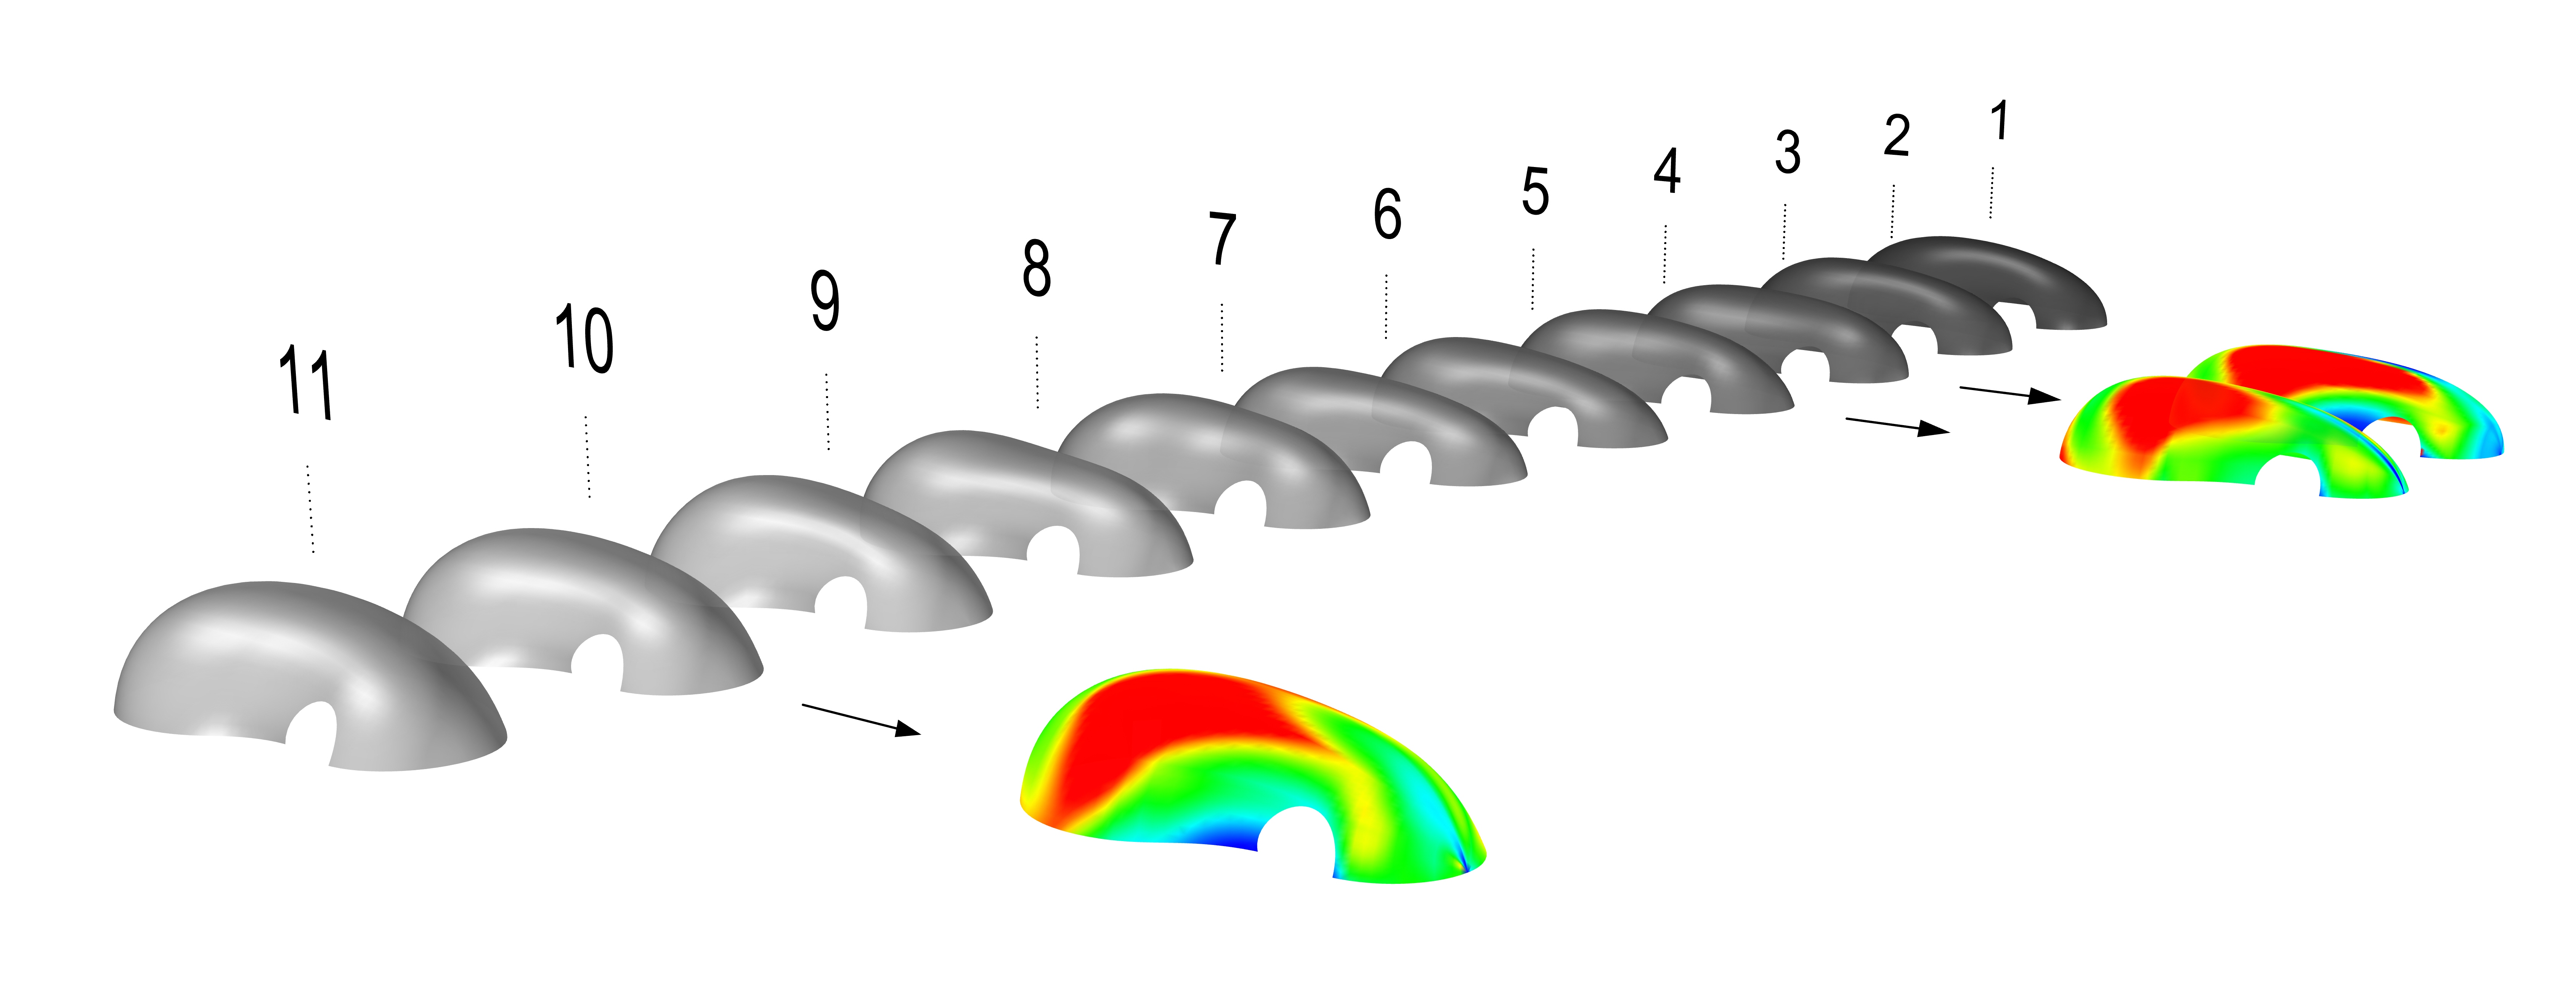
\includegraphics[width=\textwidth]{curvature_analysis}
% \caption[Benchmarking shapes regarding their curvature]{Benchmarking shapes regarding their minimum principal curvature.}
% \label{fig:shape_bench}
% %\end{fullpage}
% \end{figure}

\subsection{Meshing the surface}
%------------------------------------------
During the second step, the candidate surface is meshed and the mechanical potential of the resulting grid is evaluated. At this stage, the probability of a given mesh leading to the generation of a viable gridshell structure is estimated. Simultaneously, meshes are compared according to their architectural relevance.

In this step, the geometric curvature of the polylines drawn on the surface is an appropriate criterion to characterize the mechanical potential of the grid. Unlike the previous step, this criterion takes into account the curvature of the studied mesh and not the minimum principal curvature. In particular, it has to be ensured that the following condition is satisfied everywhere~:
\begin{equation}
	\mathrm{E} \cdot   \frac{r}{R_{spline}}  <   \frac{\sigma_{k,flex}}{\gamma_{lt}}
	\label{eq:crit_2}
\end{equation}
where $R_{spline}$ is the spline’s local curvature radius. The mesh is obtained by the compass method (see below), which develops a regularly spaced grid on a surface from two secant curves lying on the surface and called \emph{directrix}. I implemented this method, proposed by \citet{IL10}, for the Solidays gridshell in 2011 \cite{DuPeloux2011}.\footnote{This method was also used at the laboratoire Navier by \citef{Bouhaya2014} and more recently by \citef{Masson2017b}.} The method guarantees that the grid is made of parallelograms when developed in a plane. This geometric property is exactly what we are looking for to ensure the necessary degree of freedom of the grid responsible for its deployment (see \cref{sec=swivel}). For a given shape, there are an infinite number of possible meshes. The goal of the method is to identify at least one grid which satisfies both the architectural and the structural requirements.

% \begin{figure}[t]
%      	\centering
% %	\begin{fullpage}
% 		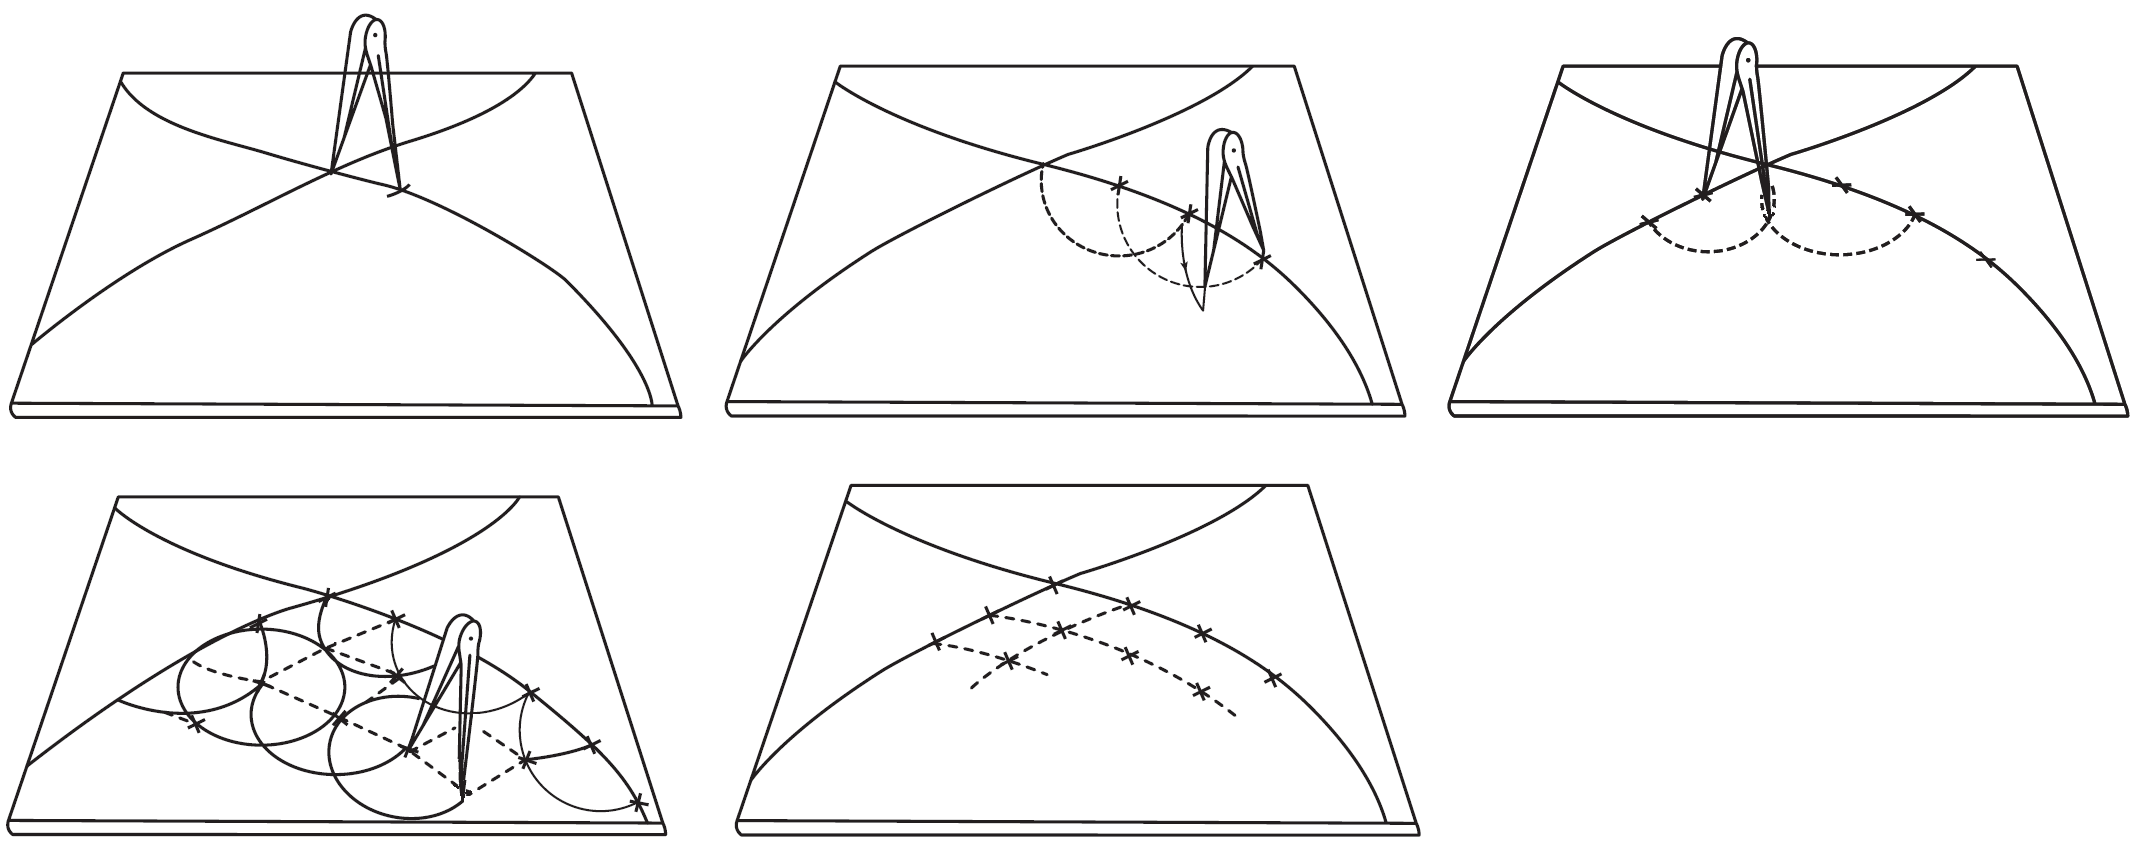
\includegraphics[width=0.8\textwidth]{compass_method.png}
% 		\caption[How the compass method works]{How the compass method works.}
% 		\label{fig:compass_method}
% 		%
% 		\vspace{0.75cm}
% 		%
% 		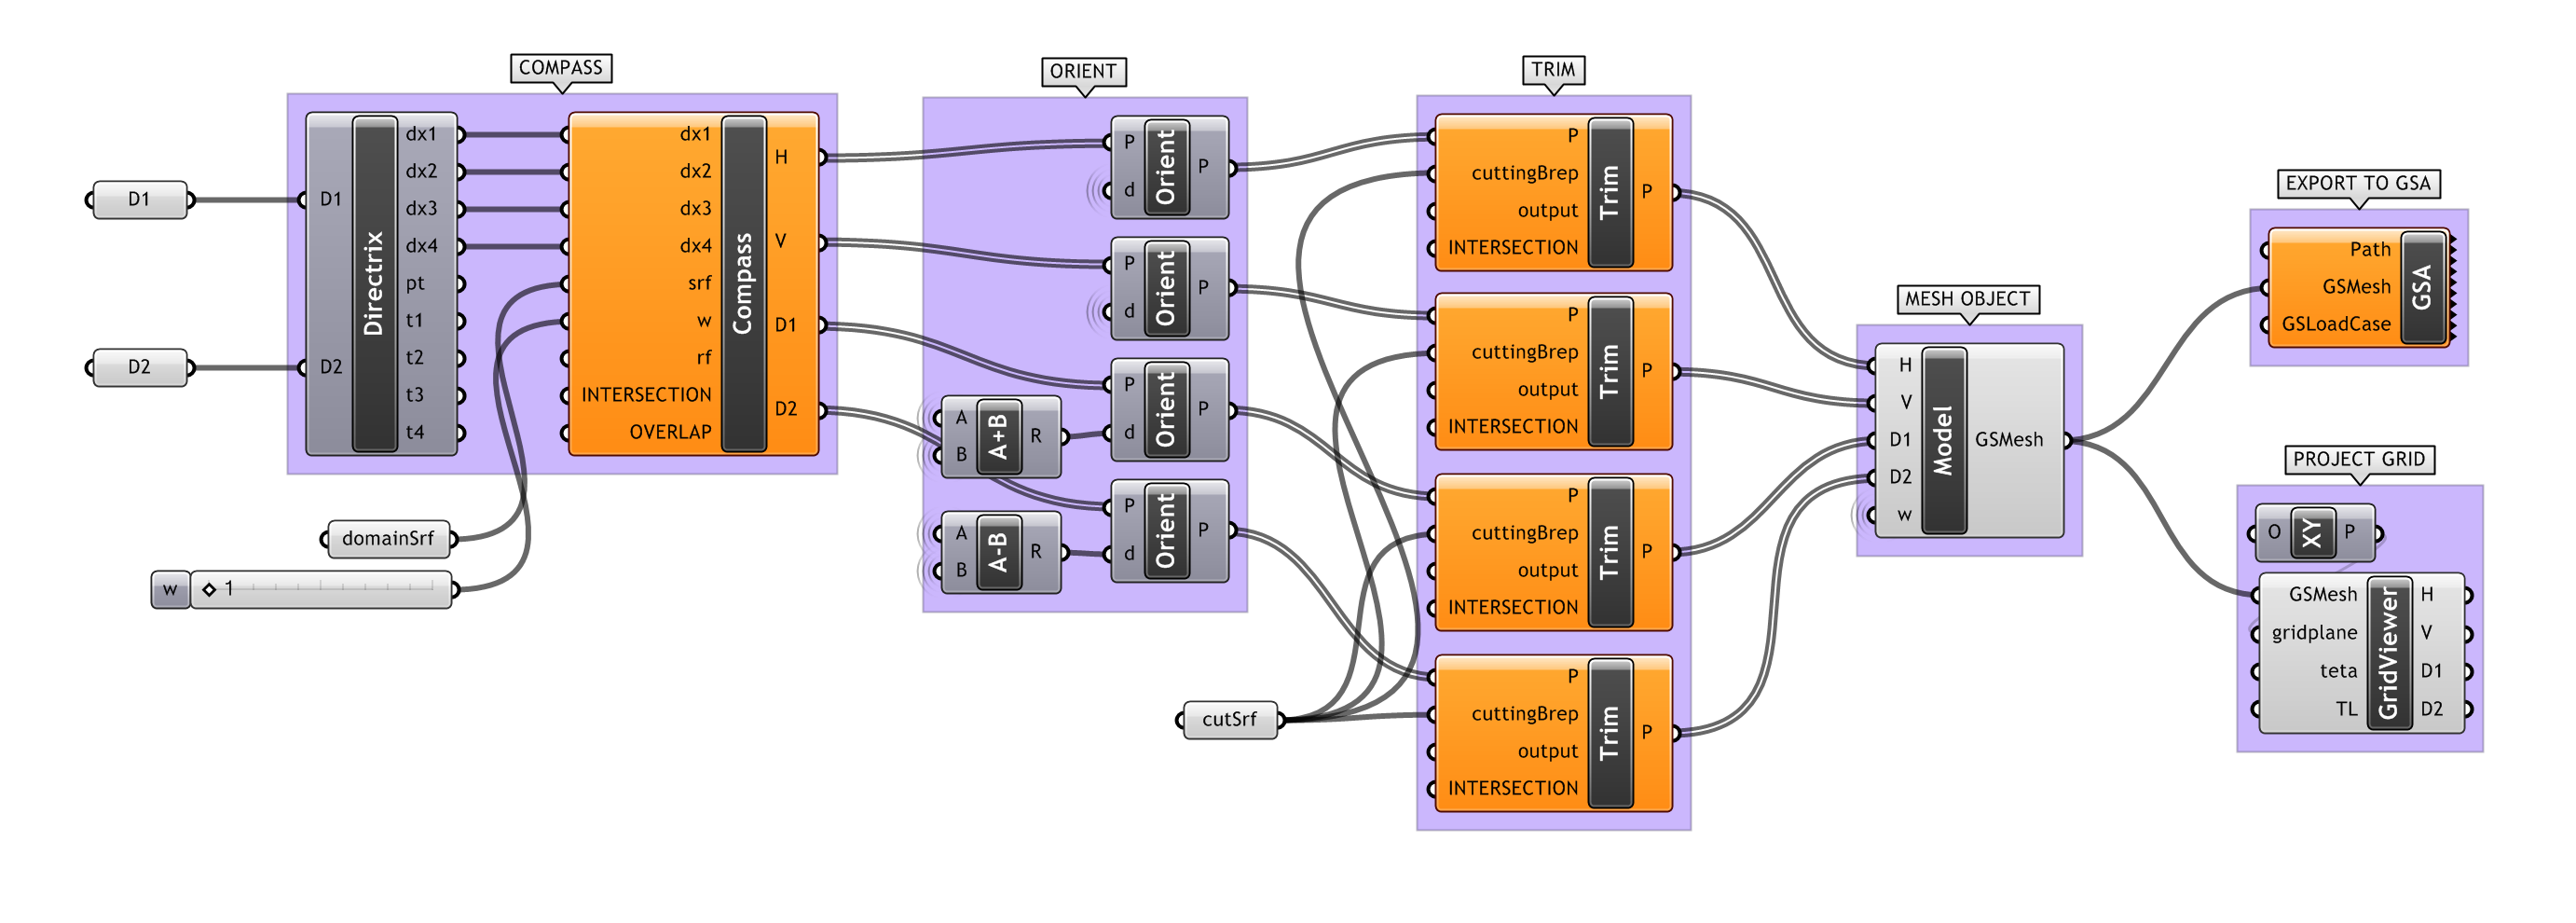
\includegraphics[width=1\textwidth]{canevas.png}
% 		\caption{Meshing software as a plugin for \emph{Grasshopper}.}
% 		\label{fig:canevas}
% %	\end{fullpage}
% \end{figure}

\subsubsection{Compass method}\label{sec=compass}
This process propagates a two way mesh of constant pitch on any NURBS surface (see \cref{fig:compass_method}). Two secant directrices are drawn on the surface to mesh. These curves mark the boundary of four quadrants. Each half directrix is then subdivided with a compass of constant distance (the pitch). Finally, from two consecutive half directrix quadrants are meshed with the same compass distance.

The compass method does not allow to spread the mesh everywhere on a given surface because it stops when a directrix reaches the boundary of the surface. Only a portion of the surface can be meshed and the covered area varies according to the chosen set of directrices. To overcome this difficulty, we consider the gridshell surface (see \cref{fig:compass_a}) as a part of a larger domain surface (see \cref{fig:compass_c}). Trimmed by a plane, this domain surface should give back the intended shape to build (see \cref{fig:compass_b}). Therefore, it is possible to mesh the domain surface (see \cref{fig:compass_d}) and to retrieve a Chebyshev net (that is an equilateral mesh) that cover completely the initial surface (see \cref{fig:compass_f}).

The method is easily extended to meshes with variable pitch. This idea was explored to find optimal grids with genetic algorithm by \citet{Bouhaya2014}. It is worthwhile to mention an attempt to extend this method for multilayer Chebyshev grids by \citet{Lefevre2015}.

\blankpage{
	\hbox{}\thispagestyle{empty}
	\setlength{\tmpwidth}{6cm}
	\AddToShipoutPictureBG*{%
		%%
		\intersectnode{PPtr |- CAtl}{Pt}
		\Photo[
			node=Pt,
			anchor=north east,
			gopt={width=\tmpwidth},
			]{compass_3.png}%
		\savenodes{C}
		\Photo[
			node=Ctl,
			anchor=north east,
			xshift=-\PhotoSkip,
			% yshift=\PhotoBigSkip,
			gopt={width=\tmpwidth},
			]{compass_2.png}%
		\savenodes{B}
		\Photo[
			node=Btl,
			anchor=north east,
			xshift=-\PhotoSkip,
			gopt={width=\tmpwidth},
			]{compass_1.png}%
		\savenodes{A}
		%%
		\intersectnode{PPtl |- Abr}{Pt}
		\Photo[
			node=Pt,
			anchor=north west,
			yshift=-\PhotoBigSkip,
			gopt={width=\tmpwidth},
			]{compass_4.png}%
		\savenodes{D}
		\Photo[
			node=Dtr,
			anchor=north west,
			xshift=\PhotoSkip,
			% yshift=\PhotoBigSkip,
			gopt={width=\tmpwidth},
			]{compass_5.png}%
		\savenodes{E}
		\Photo[
			node=Etr,
			anchor=north west,
			xshift=\PhotoSkip,
			% yshift=\PhotoBigSkip,
			gopt={width=\tmpwidth},
			]{compass_6.png}%
		\savenodes{F}
		\intersectnode{Ftr |- CAbl}{Pt}
		\Photo[
			node=Pt,
			anchor=south east,
			xshift=0mm,
			yshift=\PhotoBigSkip,
			gopt={width=0.6\textwidth},
			]{compass_method.png}%
		\savenodes{G}
		%%%%%%
		\PhotoCaptionRef[
			hrefnode=CAtl,
			node=Atl,
			anchor=south west,
			yshift=\PhotoRefSkip,
			phantom=true,
			]{figure}{}{The compass method step by step}{fig:stepbystep}
		\PhotoCaptionRef[
			hrefnode=Atl,
			node=Atl,
			anchor=south west,
			yshift=\PhotoRefSkip,
			]{subfigure}{}{Target shape}{fig:compass_a}
		\PhotoCaptionRef[
			hrefnode=Btl,
			node=Btl,
			anchor=south west,
			yshift=\PhotoRefSkip,
			]{subfigure}{}{Domain and trimming surfaces}{fig:compass_b}
		\PhotoCaptionRef[
			hrefnode=Ctl,
			node=Ctl,
			anchor=south west,
			yshift=\PhotoRefSkip,
			]{subfigure}{}{Secant directrices}{fig:compass_c}
		\PhotoCaptionRef[
			hrefnode=Dtl,
			node=Dtr,
			anchor=south east,
			yshift=\PhotoRefSkip,
			]{subfigure}{}{Resulting mesh}{fig:compass_d}
		\PhotoCaptionRef[
			hrefnode=Etl,
			node=Etr,
			anchor=south east,
			yshift=\PhotoRefSkip,
			]{subfigure}{}{Trimmed mesh}{fig:compass_e}
		\PhotoCaptionRef[
			hrefnode=Ftl,
			node=Ftr,
			anchor=south east,
			yshift=\PhotoRefSkip,
			]{subfigure}{}{Final grid}{fig:compass_f}
		\intersectnode{Atl |- Fbr}{Pt}
		\PhotoTextBox[
			node=Pt,
			anchor=north west,
			yshift=-\PhotoBigSkip,
			width=10cm,
			border=false,
			]{%
				\figurecaption{fig:stepbystep}\par
				\figurecaption{fig:compass_a}\par
				\figurecaption{fig:compass_b}\par
				\figurecaption{fig:compass_c}\par
				\figurecaption{fig:compass_d}\par
				\figurecaption{fig:compass_e}\par
				\figurecaption{fig:compass_f}
			}
		%%%
		\intersectnode{Gtl |- CAbr}{Pt}
		\PhotoCaptionRef[
			hrefnode=Pt,
			node=Pt,
			anchor=south west,
			% yshift=\PhotoRefSkip,
			phantom=true,
			]{figure}{}{Principle of the compass method}{fig:compass_method}
		\PhotoTextBox[
			node=Pt,
			anchor=south west,
			% yshift=-\PhotoSkip,
			width=10cm,
			border=false,
			]{%
				\figurecaption{fig:compass_method}
			}
	}
}

\subsubsection{Numerical tool}
Here, a specific program developed by \citet{DuPeloux2011} for \rhino{} and \grasshopper{} allows the generation of this kind of mesh on any non-uniform rational B-spline surface (NURBS). It performs the following elementary operations~: surface meshing with the compass method, trimming, control of the geometry’s integrity and flattening of the grid (see \cref{fig:stepbystep,fig:grid_diff}). The tool also generates automatically a text file, which can be imported into a structural analysis software, containing all the required information to build programmatically the analysis model and then perform the form-finding of the structure (see \cref{fig:canevas}). In particular, an add-on feature facilitates loads application of various complexities (snow, wind, etc.), which is otherwise difficult in conventional analysis softwares for freeform structures. However, the tool does not provide any computation facilities itself and this is exactly the goal of the second part of this thesis.

\subsection{Form-finding and bending prestress}\label{sec=form-finding}
%------------------------------------------
In the previous steps, the initial form was optimized and promising meshes for the materialization of the future gridshell were identified. However, the produced meshes do not take into account any of the mechanical reality, because only geometrical rules were used in their generation. The form-finding step consists precisely in finding the geometry of the grid at mechanical equilibrium, and the corresponding permanent bending stresses. The calculation is performed numerically thanks to a dynamic relaxation algorithm with kinetic damping and comprise the following steps~:
\begin{itemize}
\item The grid is bent by a set of applied displacements from its resting position to the compass position.
\item The grid is then relaxed until it falls in its mechanical equilibrium.
\item Bending stresses of the triangulation are calculated relative to the geometry of the equilibrium.
\item Geometry and bending stresses of the triangulation are re-injected into the model in step~2.
\end{itemize}

\blankpage{
	\hbox{}\thispagestyle{empty}
	\setlength{\tmpwidth}{6cm}
	\AddToShipoutPictureBG*{%
		%%
		\intersectnode{PPtr |- CAtl}{Pt}
		\Photo[
			node=CAc,
			anchor=center,
			gopt={width=0.9\textheight, angle=90},
			]{gsa.png}%
		\savenodes{A}
		\Photo[
			node=CAtr,
			anchor=north east,
			xshift=2\PhotoBigSkip,
			gopt={width=3cm, angle=0},
			]{gsa_scale.png}%
		\savenodes{B}
		\PhotoCaptionRef[
			hrefnode=Atl,
			node=Atl,
			anchor=north east,
			phantom=true,
			% yshift=\PhotoRefSkip,
			]{figure}{}{Permanent bending stresses in the structure under self-weight}{fig:gsa}
		\PhotoTextBox[
			node=CAbl,
			anchor=south west,
			border=false,
			]{%
				\figurecaption{fig:gsa}
			}
	}
	\afterpage{%
		
		\AddToShipoutPictureBG*{% 
			\setlength{\tmpwidth}{(\textwidth-3\PhotoBigSkip)/2}
			\Photo[
				node=CAt,
				anchor=north east,
				xshift=-\PhotoBigSkip/2,
				gopt={width=\tmpwidth},
				]{eccentricity_1.png}%
			\savenodes{A}
			\Photo[
				node=CAt,
				anchor=north west,
				xshift=\PhotoBigSkip/2,
				gopt={width=\tmpwidth},
				]{eccentricity_2.png}%
			\savenodes{B}
			%%
			\PhotoCaptionRef[
				hrefnode=Atl,
				node=Atl,
				anchor=south east,
				yshift=\PhotoRefSkip,
				phantom=true,
				]{figure}{}{Reconstruction of the full 3D geometry}{fig:eccentricity}
			\PhotoCaptionRef[
				hrefnode=Atl,
				node=Atr,
				anchor=north east,
				% yshift=\PhotoRefSkip,
				]{subfigure}{}{Wire frame}{fig:eccentricity_a}
			\PhotoCaptionRef[
				hrefnode=Btl,
				node=Btr,
				anchor=north east,
				% yshift=\PhotoRefSkip,
				]{subfigure}{}{Full 3D}{fig:eccentricity_b}
			\intersectnode{CAtl |- Abr}{Pt}
			\PhotoTextBox[
				node=Pt,
				anchor=north west,
				yshift=-\PhotoSkip,
				width=10cm,
				border=false,
				]{%
					\figurecaption{fig:eccentricity}\par
					\figurecaption{fig:eccentricity_a}\par
					\figurecaption{fig:eccentricity_b}\par
				}
		}
		\setlength{\tmpheight}{\PhotoHeight}
		\addtolength{\tmpheight}{4\PhotoBigSkip}
		\hbox{\vspace{\tmpheight}}
	}
}

Two analysis models were built during this process to study the structure with and without bracing tubes.

The computations were realized with the form-finding module of the software Oasys GSA.\footnote{\url{http://www.oasys-software.com/products/engineering/gsa-suite.html}} It relies on a 6-DOF dynamic relaxation algorithm with either viscous or kinetic damping such as the one introduced in \citeyear{Adriaenssens2000} by \citet{Adriaenssens2000}. In practice, making the computations to converge was a really difficult and time-consuming task, highlighting the necessity of a dedicated form-finding tool with a higher level of interactivity. Moreover, coupling between rotational and translational degrees of freedom can cause ill-conditioning problems, which was already noticed by \citet{Adriaenssens2001}. In the same paper, they proposed a 3-DOF element valid for torsion-free cases. Simpler and faster, it is also a lot more stable. This element was reused and extended later for the form-finding of elastic gridshells in composite materials with complex connections by \citet{Douthe2007}. To tackle numeric instabilities the model had to be simplified~:
\begin{itemize}
\item Connections between elements were modeled as rotation-free joints, enforcing only position constrains with out taking into account the eccentricity between the tubes. This becomes a problem when it comes to evaluating the stability of the gridshell as eccentricity can plays a major role \cite{Lefevre2015}. This is also problematic when determining the production length of the tubes and the position of the anchorages (see \cref{sec=asbuilt}).
\item The triangulation could not be embedded from the start in the model and had to be treated separately and re-injected later on.
\end{itemize}

The form-finding process should not be regarded as a pure computational stage were only the equilibrium shape has to be found while all other design parameters are fixed. Indeed, as the goal is to find a suitable geometry with the most relaxed permanent bending stresses in the structure, this process could itself be employed to explore optimal geometries that will lead to more relaxed static equilibriums. In the present project the supports were allowed to move slightly around their target position by the mean of spring supports with orthotropic stiffness. This allowed to decrease the overall level of permanent bending stress in the tubes while granting very minor changes in the geometry.

Finally the process converges when the shape and the pattern drawn by the mesh are suitable for the architect while the permanent bending stresses are acceptable for the tubes (see \cref{sec=safety}). The end results for this stage are presented in \cref{fig:gsa}. Note the smoothness of the mesh and the convergence of the tubes near the altar. Bending stresses are well distributed and inferior to the maximum design stress allowed (\SI{133}{MPa} in that case). Only few tubes are heavy loaded, in the areas where the curvature is the highest.

\subsection{As-built geometry}\label{sec=asbuilt}
 %-------------------------------------
Although, the eccentricity ($e = \SI{136}{\mm}$) remains small compared with the span of the shell ($l =\SI{17}{m}$), it is not negligible compared with the mesh size ($w = \SI{1.0}{m}$). Thus, the tube lengths and anchorage positions could not be determined with sufficient accuracy without taking into account the thickness of the structural grid due to this eccentricity. The employed method, purely geometrical, assesses that the neutral fibre of the shell is equidistant from the first two layers of pipes. The form-finding is performed only with those two layers. Connection axes has to be parallel to the local normal of the shell surface. This assumption was not exact, but, in this case, gave sufficient accuracy. The red pipe was offset by $-e/2$, the green by $+e/2$ and the blue by $+3e/2$ along the surface normal (see \cref{fig:eccentricity}).
% \begin{figure}[p]
%      	\centering
% 	\begin{fullpage}
% 		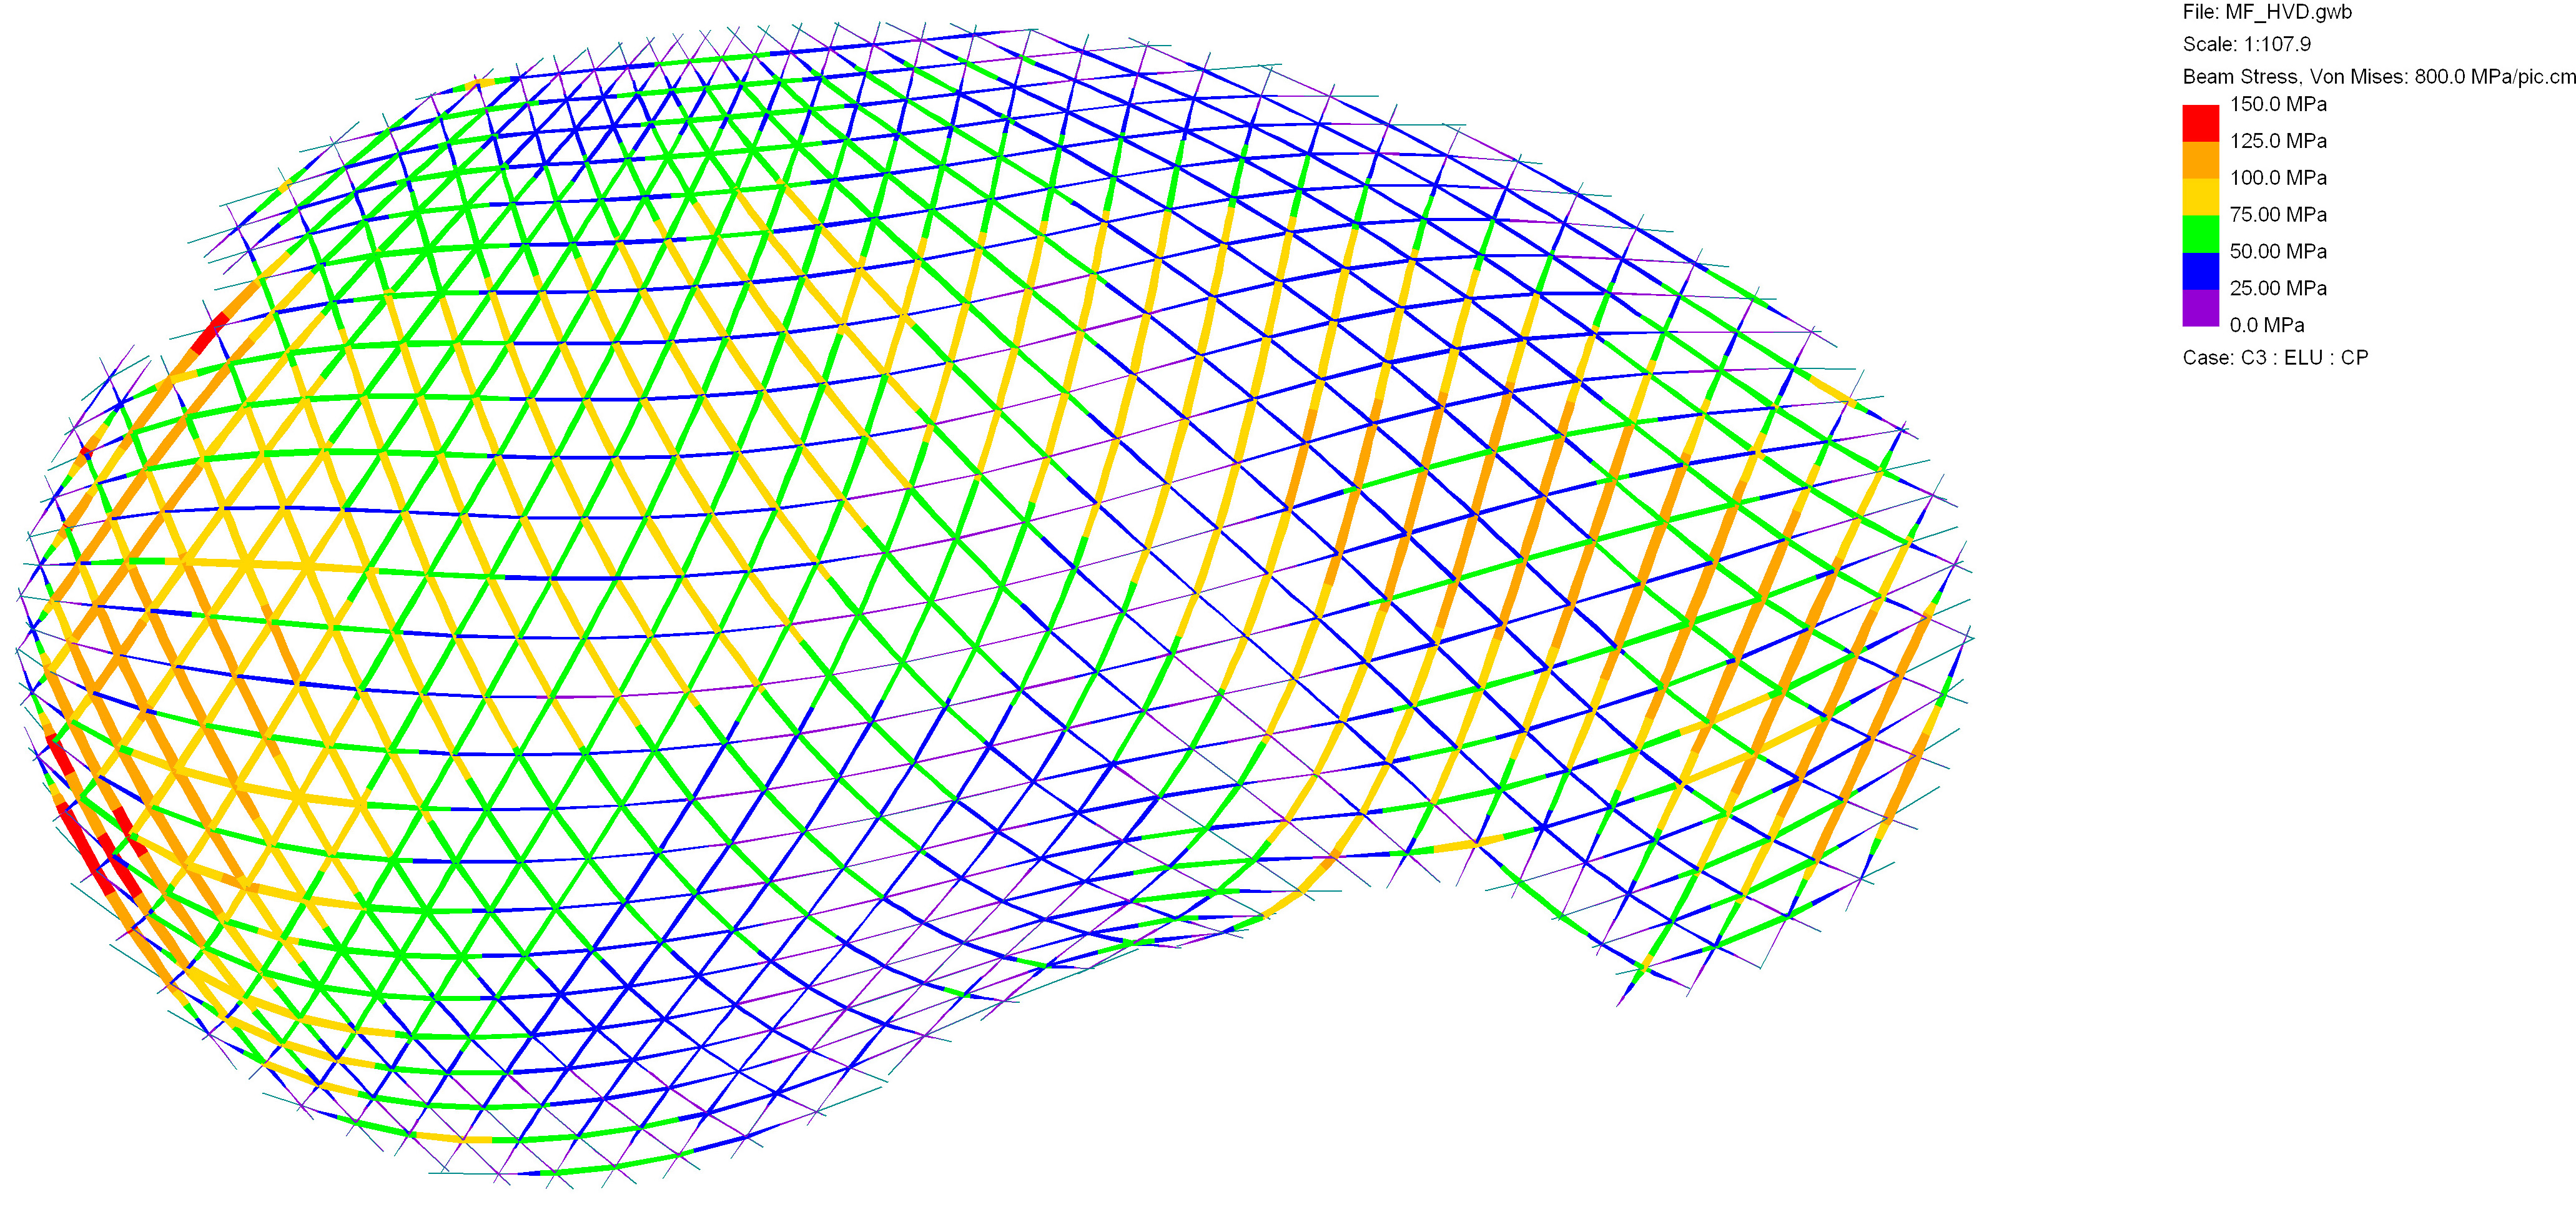
\includegraphics[width=1\textwidth]{gsa2.jpg}
% 		\caption[Permanent bending stresses in the structure under self-weight]{Permanent bending stresses in the structure under self-weight (max = \SI{130}{MPa}).}
% 		\label{fig:gsa}
% 		%
% 		\vspace{1.5cm}
% 		%
% 		\subfloat[][Wire frame]{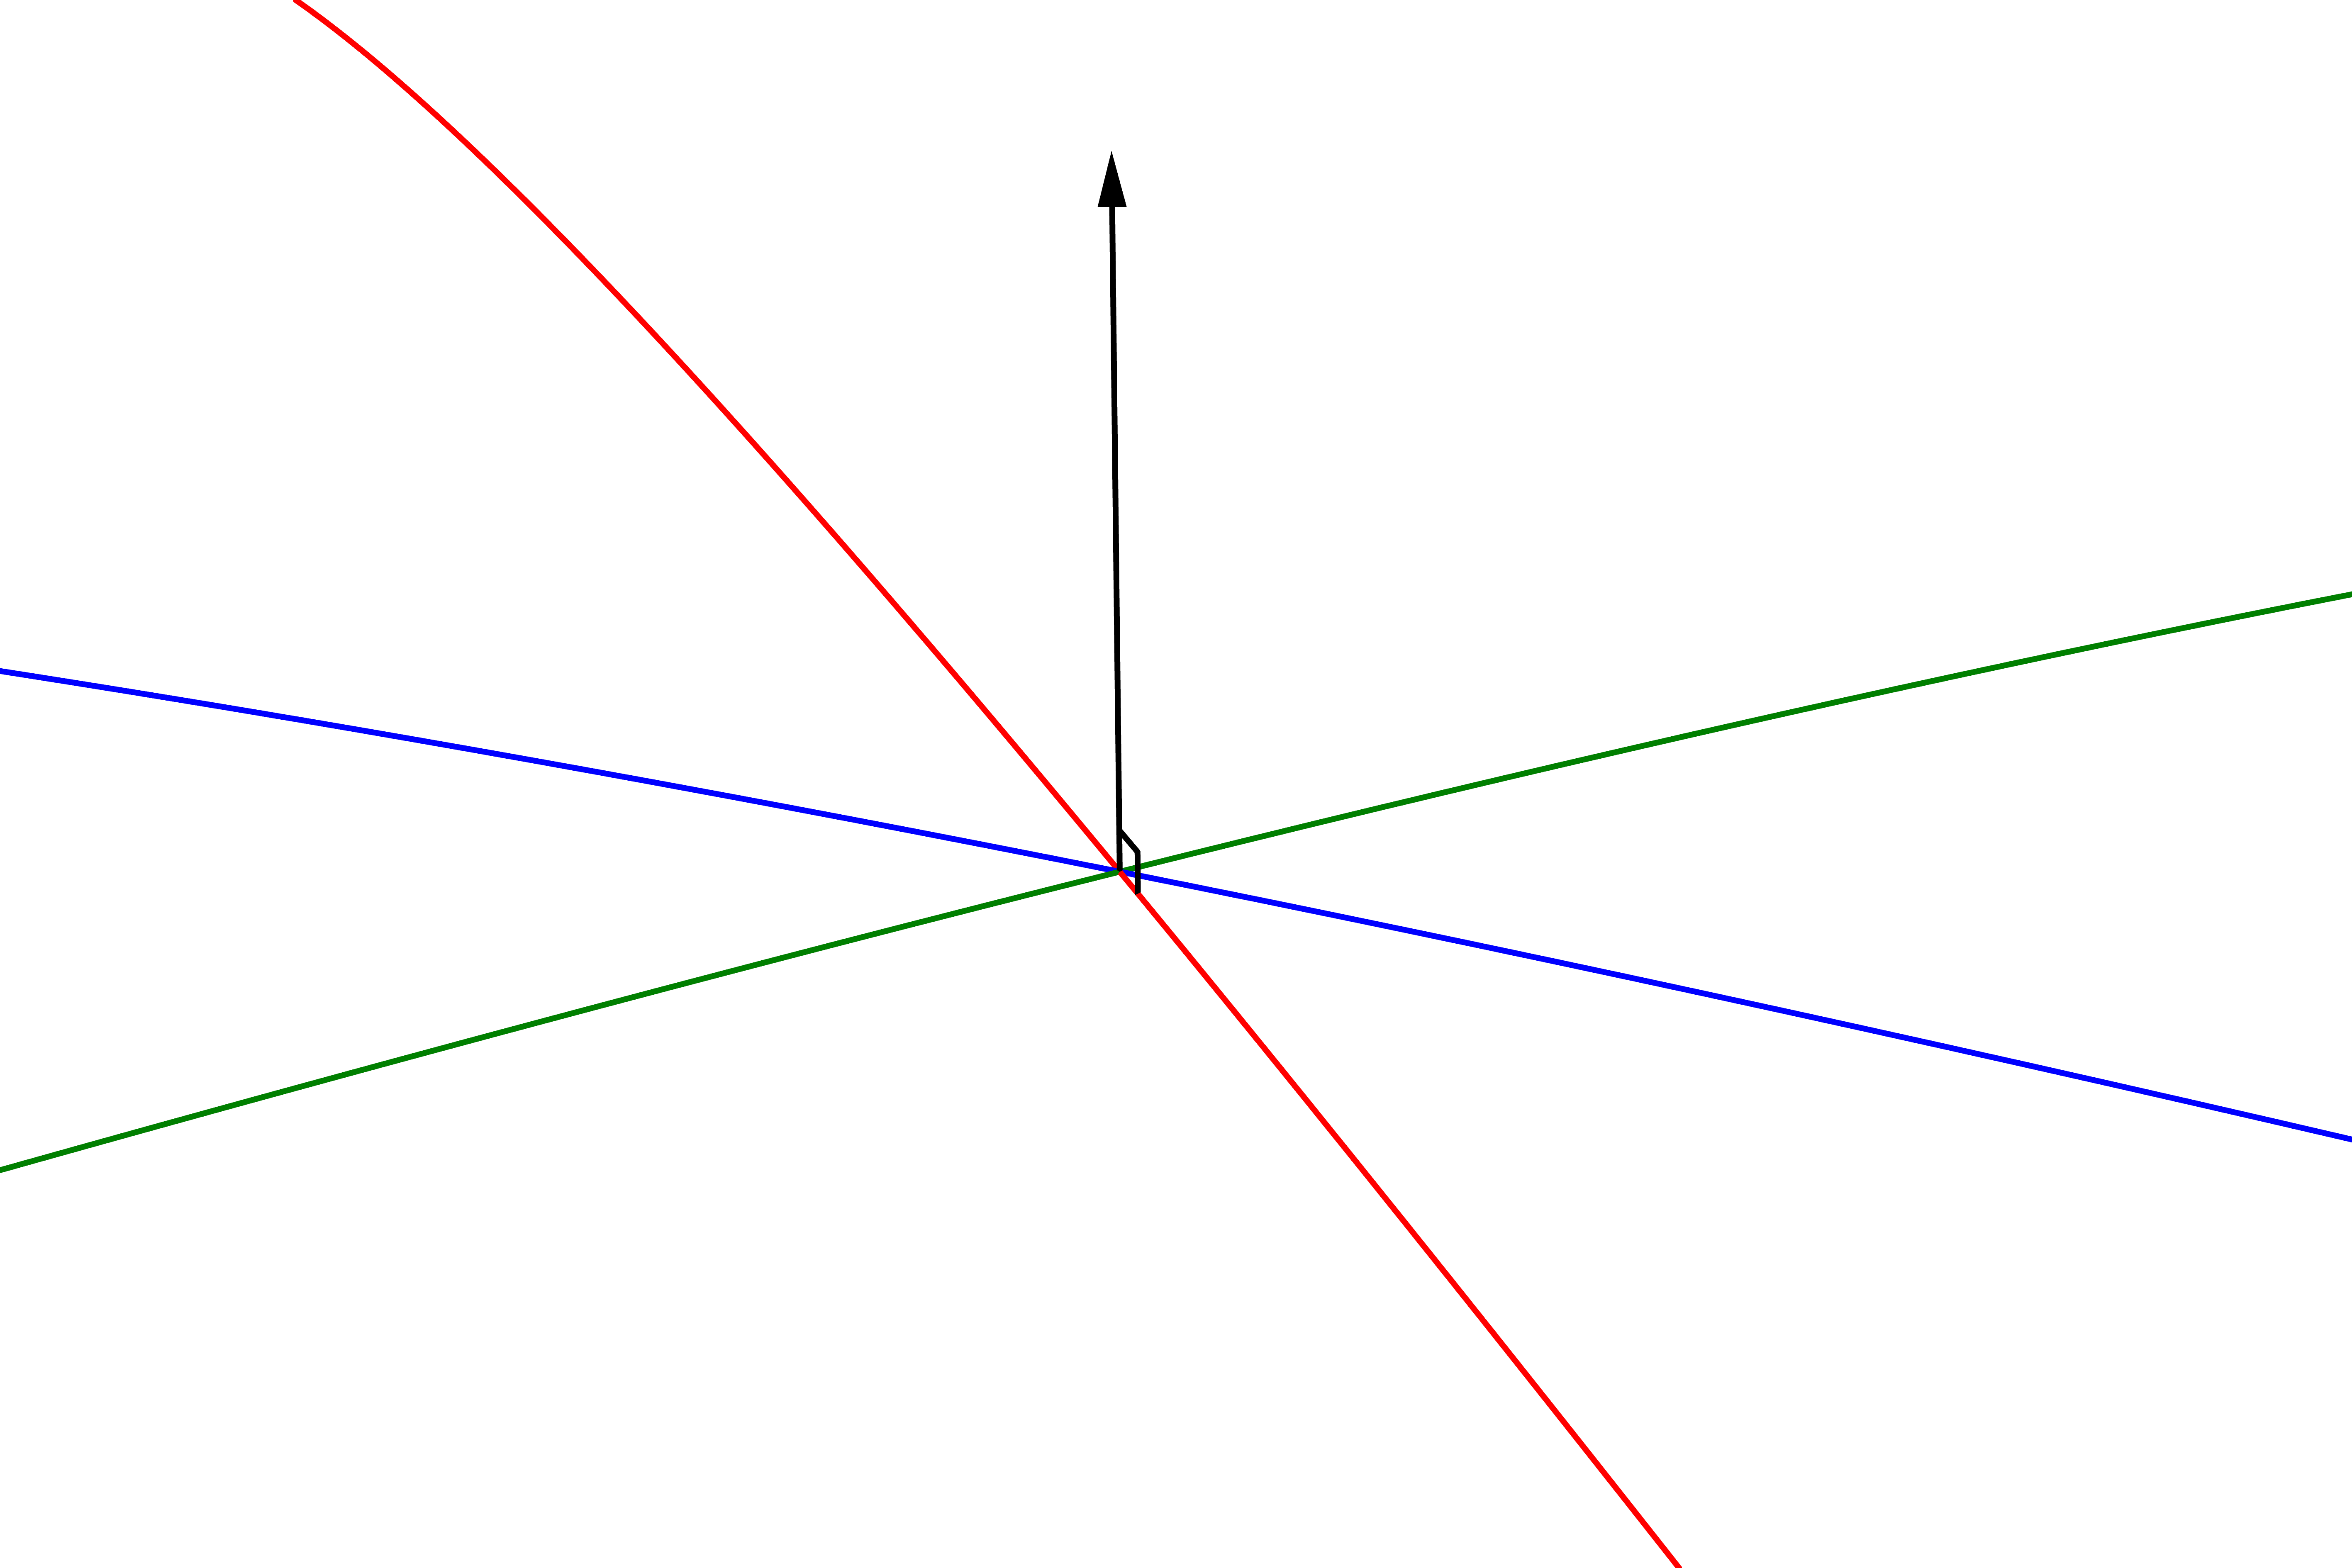
\includegraphics[width=0.48\textwidth]{eccentricity_1.png}\label{fig:eccentricity_a}}
% 		\hspace*{\fill}
% 		\subfloat[][Full 3D]{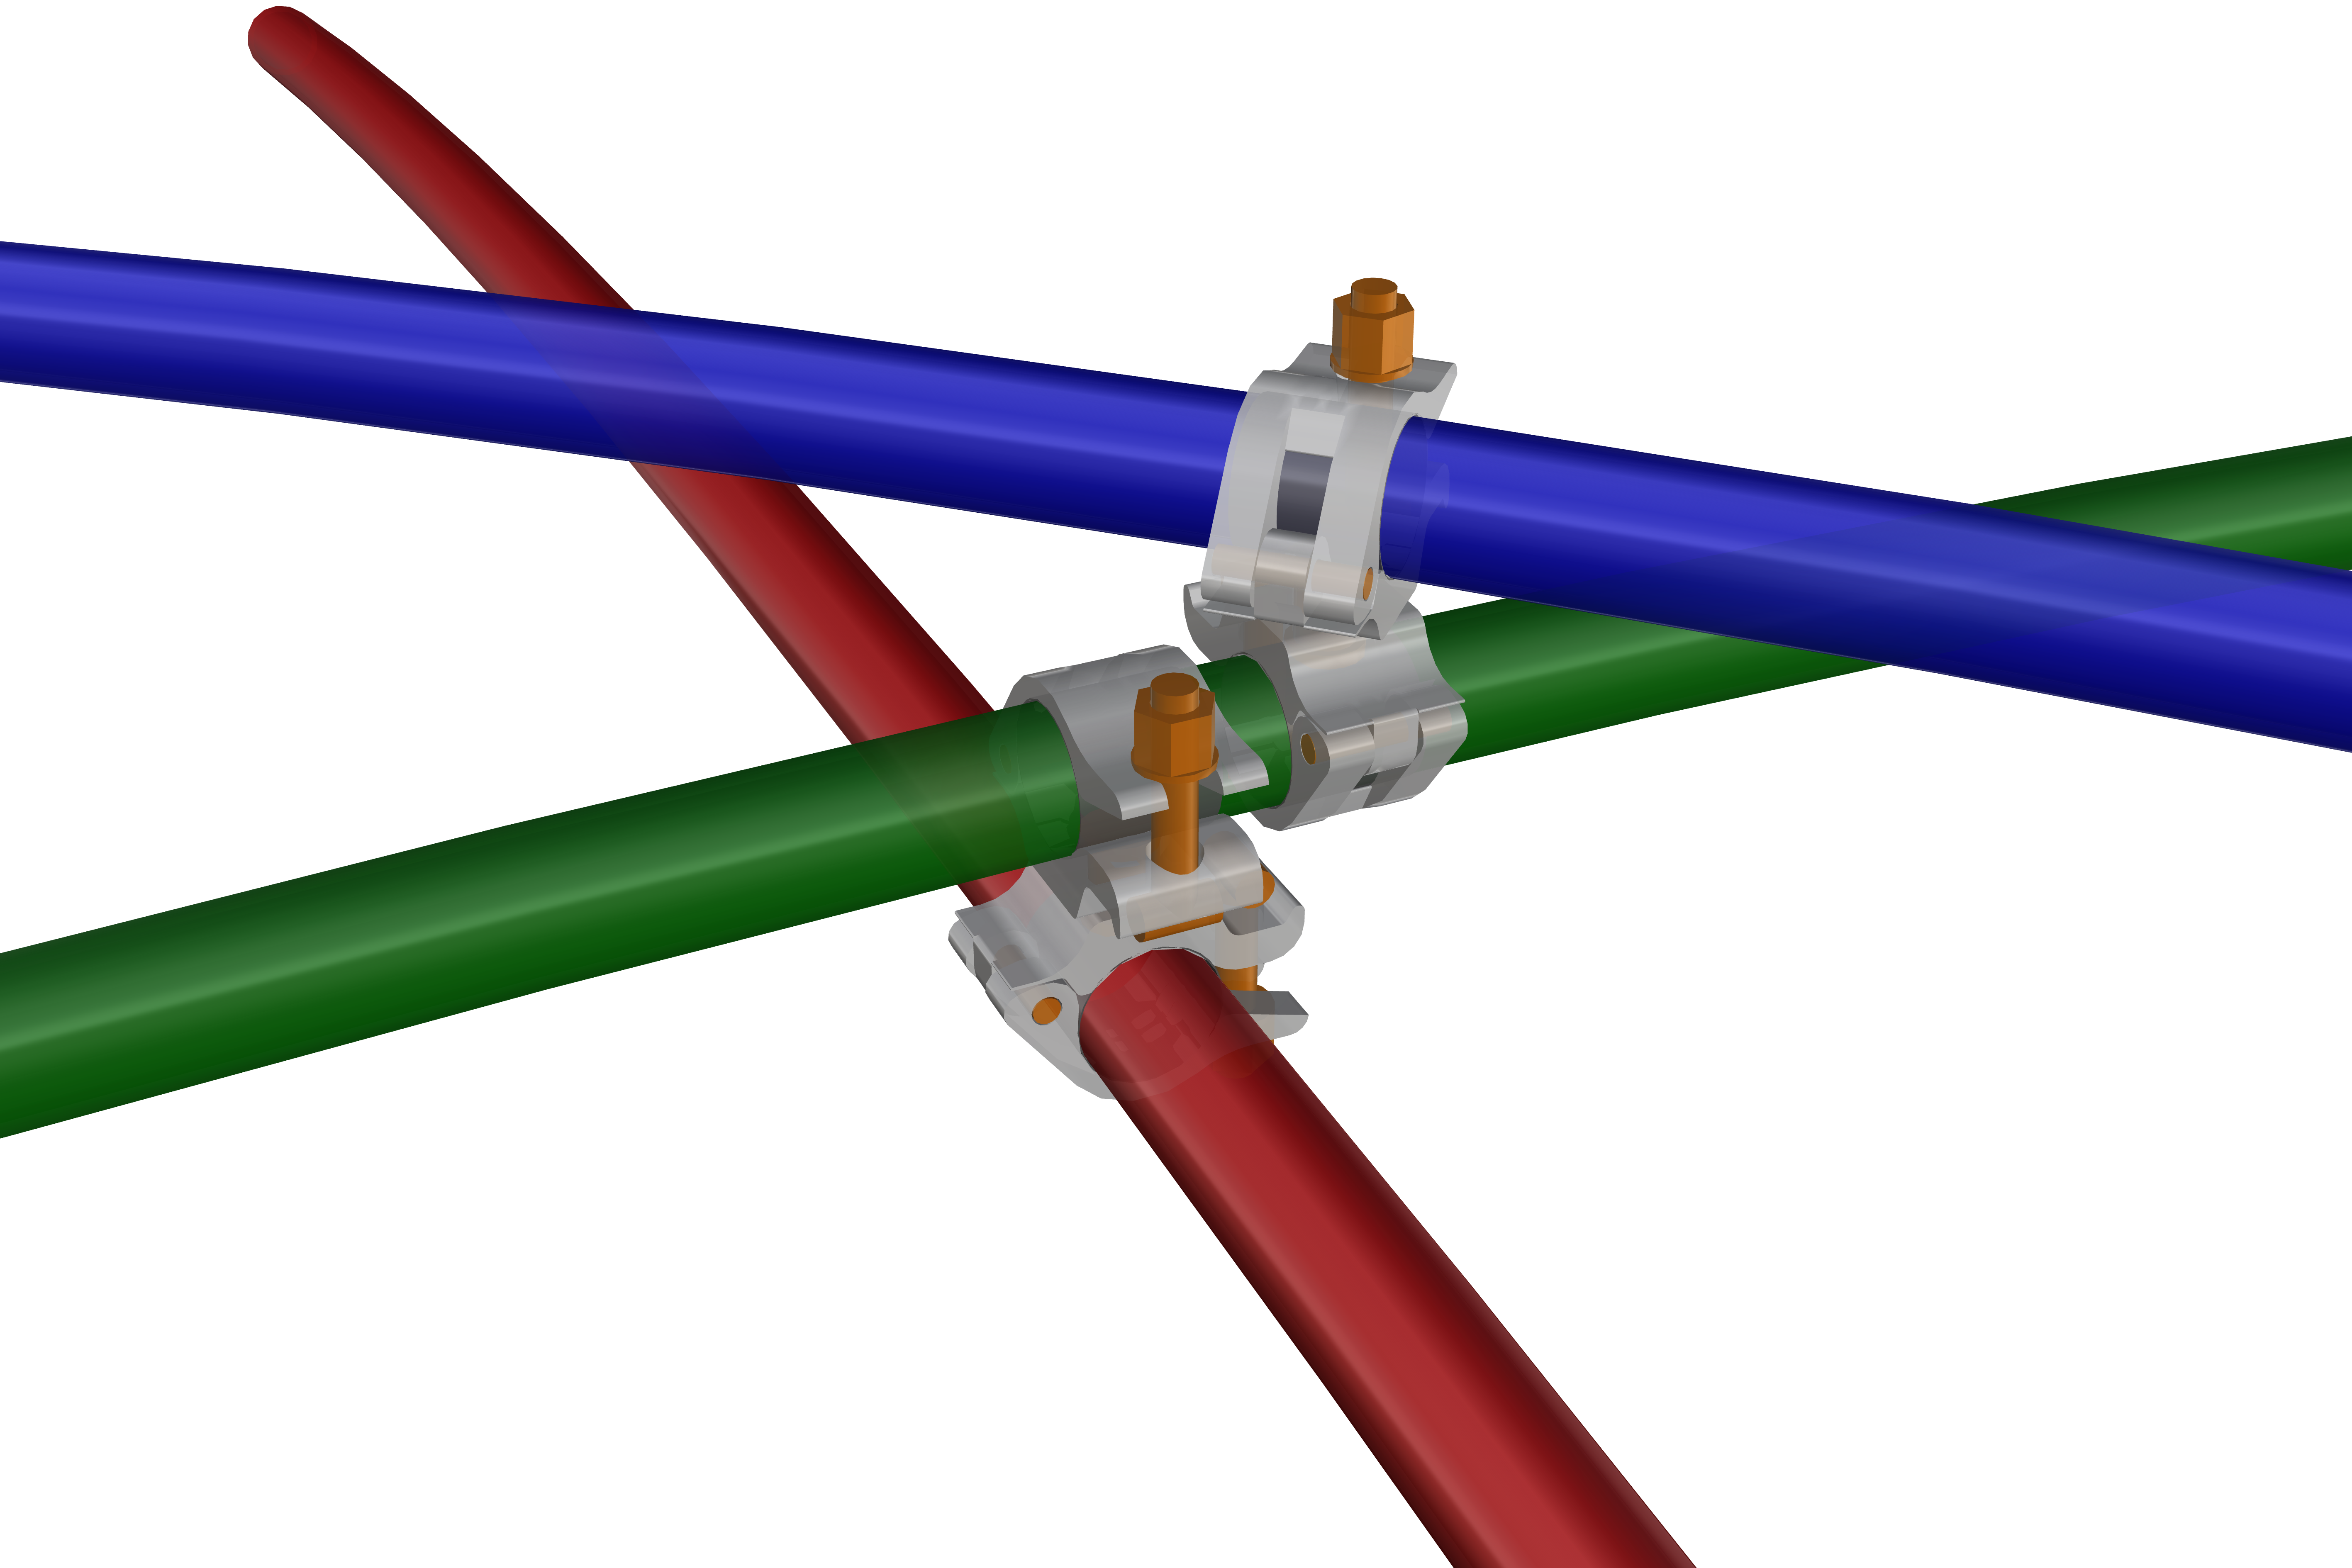
\includegraphics[width=0.48\textwidth]{eccentricity_2.png}\label{fig:eccentricity_b}}
% 		\vspace{0.5cm}
% 		\caption[Reconstruction of the full 3D geometry]{Reconstruction of the full 3D geometry.}
% 		\label{fig:eccentricity}
% 	\end{fullpage}
% \end{figure}
\subsection{Structural analysis}
%------------------------------------------
A full structural analysis is finally performed on the gridshell, using the two mechanical models created previously during the form-finding stage.
The non-braced model is used to check the grid’s behavior during the construction stages. In particular, it must be verified that the primary grid - the one with no triangulation tubes - has no risk of buckling, both for obvious safety reasons and to ensure the accuracy of the final geometry. Indeed, the more the form is likely to buckle, the more it can be triangulated in a buckled geometry different to the targeted geometry. The model with the triangulated grid is used to confirm the gridshell complies with all the structural requirements during its lifetime. Its behavior under standard loadings is evaluated.

% %\newpage \phantom{abc}
% \clearpage
\section{Designing with GFRP materials}\label{sec=design_gfrp}
%------------------------------------------
This section focuses on the GFRP tubes employed for the structure. We present how we managed to deal with this composite material in the eyes of the existing regulatory framework although there is no applicable norms for composite materials (see \cref{sec=codes}). Beyond the administrative strategy, we present how their flexural strength was evaluated (see \cref{sec=flex}) and how the corresponding partial safety factors were detremined (see \cref{sec=safety}).

\subsection{Properties of the tubes}\label{sec=gfrp}
% -------------------------------------------------------
The technical properties of the tube employed for this project are given in \cref{tab:tube}. Although these data were provided by the manufacturer at the time of the project, a test campaign was done to verify the flexural resistance of the tubes taking into account the influence of the swivel couplers clamped on the tubes (see \cref{sec=flex}).
%The characterization of this material is presented in detail in this paper \cite{Kotelnikova2012}.
\blankpage{
	\hbox{}\thispagestyle{empty}
	\AddToShipoutPictureBG*{
		\SBox[%
			node=CAc,
			anchor=center,
			]{%
				\ra{1.1}
				\begin{tabular}{@{}l l r @{}}
					\toprule
					Item 							& Standard	 	& Polyester Mat-Roving-Mat \\
					\midrule
					External diameter 				&				& \SI{41.7}{\mm} \\
					Internal diameter 				& 				& \SI{34.7}{\mm} \\
					Wall thickness					& 				& \SI{3.5}{\mm} \\
					Section area					& 				& \SI{4.20e-2}{m^2} \\
					Section moment of inertia			&				& \SI{7.7259e-4}{m^4} \\
					Torsion constant				&				& \SI{15.4518e-4}{m^4} \\
					\midrule
					Shipping length 				& 				& \SI{12.0}{\m} \\
					Glass content by weight 			& ISO 1172		& \SI{60}{\percent}\\
					Specic weight					& ASTM D792		& \SI{1.75}{\kg/m^3}\\
					Linear weight					& 				& \SI{0.735}{\kg/lm}\\
					Coefficient of thermal expansion	& ASTM D696		& \SI{11e-6}{K^{-1}}\\
					\midrule
					Tensile strength					& ASTM D638		& \SI{400}{MPa}\\
					Tensile modulus				& ASTM D638		& \SI{26}{GPa}\\
					Flexural strength				& ASTM D790		& \SI{400}{MPa}\\
					Flexural modulus				& full bending		& \SI{25}{GPa}\\
					Compressive strength			& ASTM D695		& \SI{220}{MPa}\\
					Compressive modulus			& ASTM D695		& \SI{20}{GPa}\\
					\bottomrule
				\end{tabular}
			}
		\PhotoCaptionRef[
			node=CAtl, 
			anchor=north west, 
			% yshift=-\PhotoRefSkip,
			phantom=true,
			]{table}{}{Technical properties of the tube}{tab:tube}
		\PhotoTextBox[
			node=CAbl,
			anchor=south west,
			border=false,
			]{\tablecaption{tab:tube}}
	}
}

\subsection{Codes for composite materials}\label{sec=codes}
Beyond the technical difficulties related to both design and structural analysis of the shell, the regulatory framework was a vital issue for the success of the project. As it was the first time a structure of this kind was going to host a large number of people for over two years, the question of its reliability over time was a major issue. In order to be built, the gridshell had to comply with existing standards, which do not take into account such an innovative edifice, all in composite material. The strategy adopted to bypass this obstacle is presented herafter.

\subsubsection{First level~: administrative classification of the building}
The first level, administrative, consisted of obtaining from the French authorities an appropriate classification for the building, taking into
consideration the project’s real-time requirement~: a light-weight structure with a short lifespan. As expected, the structure was classified as a \textquote{building open to the public} (EPR in French) from the category \textquote{big tops and tents} (CTS in french) \cite{SiteSecurite}. In this classification, construction procedures and regulations are adapted to the short lifespan of buildings.

\subsubsection{Second level~: compliance with existing standards}
The second level, normative, consisted of ensuring that most of the existing regulatory framework justified the compliance of a structure that would not, at first sight, be considered by standards that do not include composite materials.

As far as possible, the design was made in compliance with the Eurocode, where the structural design is done according to the limit states under normalized loadings (self-weight, snow, wind, etc.). Although, the Eurocodes do not directly take into account composite materials, they propose some probabilistic methods to introduce new materials (EN1990, Annexe D). The mechanical properties of the GFRP pipe were determined as far as possible by tests in conformance with these methods. Alternatively, values were taken according from the Eurocomp \cite{Clarke2003}.\footnote{The Eurocomp is a kind of pre-standard intended for the structural design of buildings and civil engineering works using GFRP composites, consistent with the Eurocode approach. It is considered as the reference design code for GFRP materials.} In some cases, such as for the sleeve, the construction design also benefited from this approach.

\afterpage{%
	\enlargethispage{-6cm}
	\AddToShipoutPictureBG*{% 
		\setlength{\tmpwidth}{(\textwidth-3\PhotoBigSkip)/2}
		\SBox[%
			node=CAbl,
			anchor=south west,
			yshift=2.5cm,
			]{%
				\ra{1.1}
				\begin{tabular}{@{}l r r r r r r @{}}
					\toprule
					Connection & $\sigma_1$ & $\sigma_2$ & $\sigma_3$ & $\sigma_4$ & $\sigma_5$ & \tablebf{$\sigma_{k}$} \\
